\documentclass[10pt,mathserif]{beamer}

\usepackage{graphicx,amsmath,amssymb,psfrag,mathtools}
\usepackage{soul}
\usepackage{amsmath,amsfonts,amsthm,bbm}
\usepackage{stmaryrd}
\usepackage{subcaption}



%Code block environment
\usepackage{listings}


\definecolor{lightgrey}{gray}{0.8}
\definecolor{medgrey}{gray}{0.6}
\definecolor{darkgrey}{gray}{0.4}
\usepackage{xcolor}
\lstset { %
    backgroundcolor=\color{black!5}, % set backgroundcolor
    basicstyle=\ttfamily,
    showstringspaces=false,
    commentstyle = \ttfamily,
    commentstyle=\color{commentgreen}\ttfamily,
    morecomment=[l][\color{darkgrey}]{//},
}



\usepackage{tikz}
\usetikzlibrary{matrix,chains,positioning,decorations.pathreplacing,arrows}
\usetikzlibrary{positioning,calc}
\usepackage{tkz-euclide}
%\usetkzobj{all}





%-------------------------------------------------------------------------------
%Definition of operator font
 \usepackage[bb=boondox]{mathalfa}
%% import \varmathbb without affecting other fonts
\usepackage{xparse}
\DeclareFontFamily{U}{ntxmia}{}
\DeclareFontShape{U}{ntxmia}{m}{it}{<-> ntxmia }{}
\DeclareFontShape{U}{ntxmia}{b}{it}{<-> ntxbmia }{}
\DeclareSymbolFont{lettersA}{U}{ntxmia}{m}{it}
\SetSymbolFont{lettersA}{bold}{U}{ntxmia}{b}{it}
\ExplSyntaxOn
\NewDocumentCommand{\varmathbb}{m}
 {
  \tl_map_inline:nn { #1 }
   {
    \use:c { varbb##1 }
   }
 }
\tl_map_inline:nn { ABCDEFGHIJKLMNOPQRSTUVWXYZ }
 {
  \exp_args:Nc \DeclareMathSymbol{varbb#1}{\mathord}{lettersA}{\int_eval:n { `#1+67 }}
 }
\exp_args:Nc \DeclareMathSymbol{varbbk}{\mathord}{lettersA}{169}
\ExplSyntaxOff
%%
\makeatletter
\DeclareFontFamily{U}{tipa}{}
\DeclareFontShape{U}{tipa}{m}{n}{<->tipa10}{}
\newcommand{\arc@char}{{\usefont{U}{tipa}{m}{n}\symbol{62}}}%

\newcommand{\arc}[1]{\mathpalette\arc@arc{#1}}

\newcommand{\arc@arc}[2]{%
  \sbox0{$\m@th#1#2$}%
  \vbox{
    \hbox{\resizebox{\wd0}{\height}{\arc@char}}
    \nointerlineskip
    \box0
  }%
}
\makeatother
\newcommand{\opA}{{\varmathbb{A}}}
\newcommand{\opB}{{\varmathbb{B}}}
\newcommand{\opC}{{\varmathbb{C}}}
\newcommand{\opD}{{\varmathbb{D}}}
\newcommand{\opE}{{\varmathbb{E}}}
\newcommand{\opF}{{\varmathbb{F}}}
\newcommand{\opG}{{\varmathbb{G}}}
\newcommand{\opH}{{\varmathbb{H}}}
\newcommand{\opI}{{\varmathbb{I}}}
\newcommand{\opJ}{{\varmathbb{J}}}
\newcommand{\opK}{{\varmathbb{K}}}
\newcommand{\opL}{{\varmathbb{L}}}
\newcommand{\opM}{{\varmathbb{M}}}
\newcommand{\opN}{{\varmathbb{N}}}
\newcommand{\opO}{{\varmathbb{O}}}
\newcommand{\opP}{{\varmathbb{P}}}
\newcommand{\opQ}{{\varmathbb{Q}}}
\newcommand{\opR}{{\varmathbb{R}}}
\newcommand{\opS}{{\varmathbb{S}}}
\newcommand{\opT}{{\varmathbb{T}}}
\newcommand{\opU}{{\varmathbb{U}}}
\newcommand{\opV}{{\varmathbb{V}}}
\newcommand{\opW}{{\varmathbb{W}}}
\newcommand{\opX}{{\varmathbb{X}}}
\newcommand{\opY}{{\varmathbb{Y}}}
\newcommand{\opZ}{{\varmathbb{Z}}}
\newcommand{\opZer}{\mathbb{0}}
%-------------------------------------------------------------------------------



%-------------------------------------------------------------------------------
%Definition of other font types
\newcommand{\va}{{\mathbf{a}}}
\newcommand{\vb}{{\mathbf{b}}}
\newcommand{\vc}{{\mathbf{c}}}
\newcommand{\vd}{{\mathbf{d}}}
\newcommand{\ve}{{\mathbf{e}}}
\newcommand{\vf}{{\mathbf{f}}}
\newcommand{\vg}{{\mathbf{g}}}
\newcommand{\vh}{{\mathbf{h}}}
\newcommand{\vi}{{\mathbf{i}}}
\newcommand{\vj}{{\mathbf{j}}}
\newcommand{\vk}{{\mathbf{k}}}
\newcommand{\vl}{{\mathbf{l}}}
\newcommand{\vm}{{\mathbf{m}}}
\newcommand{\vn}{{\mathbf{n}}}
\newcommand{\vo}{{\mathbf{o}}}
\newcommand{\vp}{{\mathbf{p}}}
\newcommand{\vq}{{\mathbf{q}}}
\newcommand{\vr}{{\mathbf{r}}}
\newcommand{\vs}{{\mathbf{s}}}
\newcommand{\vt}{{\mathbf{t}}}
\newcommand{\vu}{{\mathbf{u}}}
\newcommand{\vv}{{\mathbf{v}}}
\newcommand{\vw}{{\mathbf{w}}}
\newcommand{\vx}{{\mathbf{x}}}
\newcommand{\vy}{{\mathbf{y}}}
\newcommand{\vz}{{\mathbf{z}}}

\newcommand{\vA}{{\mathbf{A}}}
\newcommand{\vB}{{\mathbf{B}}}
\newcommand{\vC}{{\mathbf{C}}}
\newcommand{\vD}{{\mathbf{D}}}
\newcommand{\vE}{{\mathbf{E}}}
\newcommand{\vF}{{\mathbf{F}}}
\newcommand{\vG}{{\mathbf{G}}}
\newcommand{\vH}{{\mathbf{H}}}
\newcommand{\vI}{{\mathbf{I}}}
\newcommand{\vJ}{{\mathbf{J}}}
\newcommand{\vK}{{\mathbf{K}}}
\newcommand{\vL}{{\mathbf{L}}}
\newcommand{\vM}{{\mathbf{M}}}
\newcommand{\vN}{{\mathbf{N}}}
\newcommand{\vO}{{\mathbf{O}}}
\newcommand{\vP}{{\mathbf{P}}}
\newcommand{\vQ}{{\mathbf{Q}}}
\newcommand{\vR}{{\mathbf{R}}}
\newcommand{\vS}{{\mathbf{S}}}
\newcommand{\vT}{{\mathbf{T}}}
\newcommand{\vU}{{\mathbf{U}}}
\newcommand{\vV}{{\mathbf{V}}}
\newcommand{\vW}{{\mathbf{W}}}
\newcommand{\vX}{{\mathbf{X}}}
\newcommand{\vY}{{\mathbf{Y}}}
\newcommand{\vZ}{{\mathbf{Z}}}

\newcommand{\cA}{{\mathcal{A}}}
\newcommand{\cB}{{\mathcal{B}}}
\newcommand{\cC}{{\mathcal{C}}}
\newcommand{\cD}{{\mathcal{D}}}
\newcommand{\cE}{{\mathcal{E}}}
\newcommand{\cF}{{\mathcal{F}}}
\newcommand{\cG}{{\mathcal{G}}}
\newcommand{\cH}{{\mathcal{H}}}
\newcommand{\cI}{{\mathcal{I}}}
\newcommand{\cJ}{{\mathcal{J}}}
\newcommand{\cK}{{\mathcal{K}}}
\newcommand{\cL}{{\mathcal{L}}}
\newcommand{\cM}{{\mathcal{M}}}
\newcommand{\cN}{{\mathcal{N}}}
\newcommand{\cO}{{\mathcal{O}}}
\newcommand{\cP}{{\mathcal{P}}}
\newcommand{\cQ}{{\mathcal{Q}}}
\newcommand{\cR}{{\mathcal{R}}}
\newcommand{\cS}{{\mathcal{S}}}
\newcommand{\cT}{{\mathcal{T}}}
\newcommand{\cU}{{\mathcal{U}}}
\newcommand{\cV}{{\mathcal{V}}}
\newcommand{\cW}{{\mathcal{W}}}
\newcommand{\cX}{{\mathcal{X}}}
\newcommand{\cY}{{\mathcal{Y}}}
\newcommand{\cZ}{{\mathcal{Z}}}
%-------------------------------------------------------------------------------




%-------------------------------------------------------------------------------
%% macros for math notions and operators
\newcommand{\EE}{{\mathbb{E}}}
\newcommand{\expec}{\mathbb{E}}
\newcommand{\Prob}{{\mathrm{Prob}}} % probability

\newcommand{\reals}{\mathbb{R}}
\newcommand{\RR}{\mathbb{R}}
\newcommand{\complex}{\mathbb{C}}
\newcommand{\CC}{\mathbb{C}}
\newcommand{\nats}{\mathbb{N}}
\newcommand{\NN}{\mathbb{N}}
\newcommand{\ZZ}{\mathbb{Z}}
\newcommand{\bigO}{\mathcal{O}}
\newcommand{\order}[1]{{\mathcal{O}\left(#1\right)}}
\renewcommand{\SS}{{\mathbb{S}}}
\newcommand{\SSp}{\mathbb{S}_{+}}
\newcommand{\SSpp}{\mathbb{S}_{++}}
\newcommand{\sign}{\mathrm{sign}}
\newcommand{\vzero}{\mathbf{0}}
\newcommand{\vone}{{\mathbf{1}}}

\renewcommand{\Re}{\operatorname{Re}} 	%Real part
\renewcommand{\Im}{\operatorname{Im}}	%imaginary part

%\newcommand{\supp}{{\mathrm{supp}}} % support
\newcommand{\range}{\mathrm{range}\,} % domain
\newcommand{\tr}{{\mathrm{tr}}} % trace
%-------------------------------------------------------------------------------





%-------------------------------------------------------------------------------
%% Theorem definitions
\setbeamertemplate{theorems}[ams style] 
\newtheorem*{theorem*}{Theorem}
%\newtheorem{lemma}{Lemma}    % already provided by amsthm
\newtheorem{proposition}{Proposition}
%\newtheorem{proof}{Proof}  % already provided by amsthm


%-------------------------------------------------------------------------------
%% operator and convex analysis definitions

\newcommand*{\fix}{\mathrm{Fix}\,}
\newcommand*{\zer}{\mathrm{Zer}\,}
\newcommand*{\gra}{\mathrm{Gra}\,}
\newcommand{\prox}{\mathrm{Prox}}
\newcommand{\proj}{\Pi}
\newcommand{\aff}{\mathrm{aff}\,}    %affine hull
\newcommand{\intr}{\mathrm{int}\,}   %interior
\newcommand{\relint}{\mathrm{ri}\,}  %relative interior
\newcommand{\dom}{\mathrm{dom}\,} % domain
\newcommand{\epi}{\mathrm{epi}\,} % epigraph
\newcommand{\dist}{\mathrm{dist}}
\newcommand{\lagrange}{\mathbf{L}}  %saddle function
\newcommand{\fitzpatrick}{\mathbf{F}}   %Fitzpatrick function
\newcommand{\vecdelay}{\boldsymbol{d}}   %vector delay
\DeclareMathOperator*{\argmin}{argmin}
\DeclareMathOperator*{\argmax}{argmax}

%-------------------------------------------------------------------------------
%SRG definitions
\newcommand{\ereal}{\overline{\mathbb{R}^2}}
\newcommand{\ecomplex}{\overline{\mathbb{C}}}
\newcommand{\binfty}{{\boldsymbol \infty}}
\newcommand{\rarc}{\mathrm{Arc}^+}
\newcommand{\larc}{\mathrm{Arc}^-}


%-------------------------------------------------------------------------------




%-------------------------------------------------------------------------------
%Miscellaneous Stuff
%% sequences
\newcommand{\itom}{_{i=1}^{m}}
\newcommand{\ieqm}{i=1,\dots,m}

% use \numberthis to add an equation number in align*
\newcommand\numberthis{\addtocounter{equation}{1}\tag{\theequation}}

\newcolumntype{P}[1]{>{\centering\arraybackslash}p{#1}}

\mode<presentation>
{
\usetheme{default}
}
\setbeamertemplate{navigation symbols}{}
\usecolortheme[rgb={0.13,0.28,0.59}]{structure}
\setbeamertemplate{itemize subitem}{--}
\setbeamertemplate{frametitle} {
	\begin{center}
	  {\large\bf \insertframetitle}
	\end{center}
}

\newcommand\footlineon{
  \setbeamertemplate{footline} {
    \begin{beamercolorbox}[ht=2.5ex,dp=1.125ex,leftskip=.8cm,rightskip=.6cm]{structure}
      \footnotesize \insertsection
      \hfill
      {\insertframenumber}
    \end{beamercolorbox}
    \vskip 0.45cm
  }
}
\footlineon


\newcommand\footlineoff{
  \setbeamertemplate{footline} {
    \begin{beamercolorbox}[ht=2.5ex,dp=1.125ex,leftskip=.8cm,rightskip=.6cm]{structure}
      \footnotesize 
      \hfill
      {\insertframenumber}
    \end{beamercolorbox}
    \vskip 0.45cm
  }
}


\newcommand\blfootnote[1]{%
  \begingroup
  \renewcommand\thefootnote{}\footnote{#1}%
  \addtocounter{footnote}{-1}%
  \endgroup
}


\AtBeginSection[] 
{ 
	\begin{frame}<beamer> 
		\frametitle{Outline} 
		\tableofcontents[currentsection,currentsubsection] 
	\end{frame} 
} 

%% wotao's preference

        % itemize, black bullet, %150 spacing between items using "witemize"
        \newenvironment{witemize}{\itemize\addtolength{\itemsep}{0.3\baselineskip}}{\enditemize}

\iffalse
        % \setbeamertemplate{itemize items}[square]
        \setbeamertemplate{itemize items}{\textbullet}
        \setbeamercolor{itemize item}{fg=black}
        \setbeamercolor{itemize subitem}{fg=black}
        \setbeamercolor{itemize subsubitem}{fg=black}
        \setbeamercolor{enumerate item}{fg=black}
        \setbeamercolor{enumerate subitem}{fg=black}
        \setbeamercolor{enumerate subsubitem}{fg=black}
        \setbeamertemplate{itemize/enumerate body begin}{\normalsize}
        \setbeamertemplate{itemize/enumerate subbody begin}{\normalsize}
        \setbeamertemplate{itemize/enumerate subsubbody begin}{\normalsize}

        % itemize enumerate use normal sized texts
        \setbeamertemplate{itemize/enumerate body begin}{\normalsize}
        \setbeamertemplate{itemize/enumerate subbody begin}{\normalsize}
        \setbeamertemplate{itemize/enumerate subsubbody begin}{\normalsize}

        % block, black over gray with no shadow
        \setbeamertemplate{blocks}[rounded][shadow=false]
        \setbeamercolor{block title}{fg=black,bg=gray!40}
        \setbeamercolor{block body}{fg=black,bg=gray!10}
\fi

\author{Ernest K. Ryu and Wotao Yin}

\date{Large-Scale Convex Optimization via Monotone Operators}


\title{\large \bfseries Scaled Relative Graphs}

\begin{document}

\frame{
\thispagestyle{empty}
\titlepage
}



\begin{frame}
\frametitle{Scaled relative graph (SRG)}

We present the SRG, which provides a correspondence between algebraic operations on nonlinear operators and geometric operations on subsets of the 2D plane. We can think of the SRG as a signature of an operator analogous to how eigenvalues are a signature of a matrix.

\vspace{0.2in}
Using the SRG and Euclidean geometry, we establish averagedness and contractiveness of FPIs.
(Geometric arguments are rigorous proofs, not mere illustrations.)
\end{frame}

\section{Basic definitions}

\begin{frame}
\frametitle{Operator classes}
$\cA$ is a class of operators if  $\cA$ is a set of operators on $\mathbb{R}^n$ for $n\in \mathbb{N}$.

(Technical detail: $\opA_1,\opA_2\in \cA$, $\opA_1\colon\reals^n\rightrightarrows\reals^n$ $\opA_2\colon\reals^m\rightrightarrows\reals^m$, and $n\ne m$ is possible.)
%For example, $\cL_1$ is the class of nonexpansive operators on \emph{all} Hilbert spaces.

\vspace{0.2in}
Given classes of operators $\cA$ and $\cB$ and $\alpha>0$, write
\begin{align*}
\cA+\cB&=\{\opA+\opB\,|\,\opA\in \cA,\,\opB\in \cB,\,\opA\colon\reals^n\rightrightarrows\reals^n,\,\opB\colon\reals^n\rightrightarrows\reals^n\}\\
\cA\cB&=\{\opA\opB\,|\,\opA\in \cA,\,\opB\in \cB,\,\opA\colon\reals^n\rightrightarrows\reals^n,\,\opB\colon\reals^n\rightrightarrows\reals^n\}\\
\opJ_{\alpha \cA}&=\{\opJ_{\alpha \opA}\,|\,\opA\in \cA,\,\opA\colon\reals^n\rightrightarrows\reals^n\}\\
\opR_{\alpha \cA}&=2\opJ_{\alpha \cA}-\opI=\{2\opJ-\opI\,|\,\opJ\in\opJ_{\alpha \cA},\,\opJ\colon\reals^n\rightrightarrows \reals^n,\,\opI\colon\reals^n\rightrightarrows\reals^n\}\\
 \cA^{-1}&=\{ \opA^{-1}\,|\,\opA\in \cA\}\\
\alpha \cA&=\{\alpha \opA\,|\,\opA\in \cA\}.
\end{align*}
\end{frame}


\begin{frame}[fragile]
\frametitle{Operator classes}
Class of $L$-Lipschitz operators:
\begingroup\makeatletter\def\f@size{8}\check@mathfonts
\begin{align*}
\cL_{L}&=\big\{\opA\colon\dom{\opA}\rightarrow\reals^n\,|\,\| \opA x-\opA y\|^2\le L^2\|x-y\|^2,\,\forall\, x,y\in\dom{\opA}\subseteq\reals^n,\,n\in \mathbb{N}\big\}.
\end{align*}
\endgroup
%where, to clarify, $\reals^n$ is an arbitrary Hilbert space.
%We call an operator a contraction if it is $L$-Lipschitz for some $L<1$, and nonexpansive if it is $1$-Lipschitz.
Class of $\beta$-cocoercive operators:
\begingroup\makeatletter\def\f@size{8}\check@mathfonts
\begin{align*}
\cC_{\beta }&=\big\{\opA\colon\dom{\opA}\rightarrow\reals^n\,|\,\langle \opA x-\opA y,x-y\rangle\ge \beta\|\opA x-\opA y\|^2,\,\forall\, x,y\in\dom{\opA}\subseteq\reals^n,\,n\in \mathbb{N}\big\}.
\end{align*}
\endgroup
Class of monotone operators:
\begingroup\makeatletter\def\f@size{8}\check@mathfonts
\begin{align*}
\cM&=\big\{\opA\colon\reals^n\rightrightarrows\reals^n\,|\,\langle \opA x-\opA y,x-y\rangle\ge 0,\,\forall\, x,y\in\dom{\opA},\,n\in \mathbb{N}\big\}.
\end{align*}
\endgroup
Class of $\mu$-strongly monotone operators:
\begingroup\makeatletter\def\f@size{8}\check@mathfonts
\begin{align*}
\cM_{\mu}&=\big\{\opA\colon\reals^n\rightrightarrows\reals^n\,|\,\langle \opA x-\opA y,x-y\rangle\ge \mu\|x-y\|^2,\,\forall\, x,y\in\dom{\opA},\,n\in \mathbb{N}\}.
\end{align*}
\endgroup
Class of $\theta$-averaged operators:
\begin{align*}
\cN_\theta=(1-\theta)\opI+\theta\cL_1.
\end{align*}
(No requirements on domain or maximality.)
\end{frame}

\begin{frame}
\frametitle{Subdifferential operator classes}
Class of $\mu$-strongly convex and $L$-smooth CCP functions on $\reals^n$:
 \[
\cF_{\mu,L}
\]
($\mu=0$ convex but not strongly convex; $L=\infty$ not-smooth.)

\vspace{0.2in}
Class of subdifferential operators:
\begin{align*}
\partial \cF_{\mu,L} = \{\partial f \,|\, f \in  \cF_{\mu,L}\}
\end{align*}
\end{frame}

\begin{frame}
\frametitle{Basic geometry}
Stewart's theorem:
%  for a triangle $\triangle ABC$ and Cevian $\overline{CD}$ to the side $\overline{AB}$,
%We quickly state Stewart's theorem \cite{stewart}, which we use for the Proof of Proposition~\ref{prop:refl-sm-coco}.
\vspace{-0.1in}
\begin{center}
\begin{tabular}{c}
\raisebox{-.5\height}{
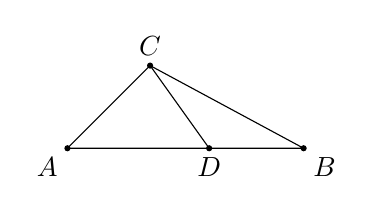
\begin{tikzpicture}[scale=1.5]
\coordinate (A) at  (-1,0);
\coordinate (B) at  (1,0);
\coordinate (C) at  (-.3,.7) ;
\coordinate (D) at  (.2,0) ;


\filldraw (A) circle ({0.6*1.5/1.5pt});
\filldraw (B) circle ({0.6*1.5/1.5pt});
\filldraw (C) circle ({0.6*1.5/1.5pt});
\filldraw (D) circle ({0.6*1.5/1.5pt});
\draw (A) node [below left] {$A$};
\draw (B) node [below right] {$B$};
\draw (C) node [above ] {$C$};
\draw (D) node [below] {$D$};

\draw  (A) -- (B)--(C)-- cycle;
\draw  (D)--(C);
\end{tikzpicture}}
\end{tabular}
\end{center}
lengths satisfy
\[
\overline{AD}\cdot
\overline{CB}^2
+
\overline{DB}\cdot
\overline{AC}^2
=
\overline{AB}\cdot
\overline{CD}^2
+\overline{AD}\cdot\overline{DB}^2
+\overline{AD}^2\cdot\overline{DB}
\]

\vspace{0.2in}

For any $a,b\in \mathbb{R}^n$, angle function:
\begin{align*}
    \angle(a,b) =
    \left\{
    \begin{array}{ll}
    \arccos\left(\tfrac{\langle a,b\rangle}{\|a\|\|b\|}\right)&\text{ if }a\ne 0,\,b\ne 0\\
    0&\text{ otherwise.}
    \end{array}
    \right.
\end{align*}


\end{frame}





\begin{frame}
\frametitle{Extended complex plane}
Extended complex plane $\ecomplex=\CC\cup\{\infty\}$ represents the 2D plane and the point at infinity.

\vspace{0.2in}

We avoid $\infty+\infty$, $0/0$, $\infty/\infty$, and $0\cdot\infty$.\\
Define $z+\infty=\infty$, $z/\infty=0$, and [$z/0=\infty$ and $z\cdot\infty=\infty$ for $z\ne 0$].

\vspace{0.2in}

Inversion map: $z\mapsto\bar{z}^{-1}$, a one-to-one map from $\ecomplex$ to $\ecomplex$. \\
%To clarify, 
%(The inversion map is well-defined at $0$ because we use the extended complex plane $\ecomplex$.)
In polar form: $re^{i\varphi}\mapsto (1/r)e^{i\varphi}$.\\


\vspace{0.2in}
(Inversion preserves angle and inverts magnitude. $\bar{z}$ is complex conjugate of $z$.)

\end{frame}



\section{Scaled relative graphs}


\begin{frame}[plain,label=slide_srg_op]
\frametitle{SRG of operators}
Let $\opA\colon\reals^n\rightrightarrows\reals^n$, $u\in \opA x$, and $v\in \opA y$.
Goal: understand change in ouputs $u-v$ relative to change in inputs $x-y$.

\vspace{0.2in}
For $x\ne y$, consider complex conjugate pair
\[
z=
\frac{\|u-v\|}{\|x-y\|}
\exp\left[\pm i \angle (u-v,x-y)\right].
\]
%where given any $a,b\in\reals^n$
%\begin{align*}
%    \angle(a,b) =
%    \left\{
%    \begin{array}{ll}
%    \arccos\left(\tfrac{\langle a,b\rangle}{\|a\|\|b\|}\right)&\text{ if }a\ne 0,\,b\ne 0\\
%    0&\text{ otherwise}
%    \end{array}
%    \right.
%\end{align*}
%denotes the angle between them.
 %(note the $\pm$) captures how large $u-v$ is relative to $x-y$ and how aligned $u-v$ is relative to $x-y$.
Magnitude $|z|=\tfrac{\|u-v\|}{\|x-y\|}$ represents size of $u-v$ relative to size of $x-y$.
Angle $\angle (u-v,x-y)$ represents how much $u-v$ is aligned with $x-y$.

\vspace{0.2in}
Equivalently, $\Re z$ and $\Im z$ respectively represent the
components of $u-v$ aligned with and perpendicular to $x-y$:
\begin{align*}
\Re z
&=
\textrm{sgn}(\langle u-v,x-y\rangle)\frac{\|\proj_{\mathrm{span}\{x-y\}}(u-v)\|}{\|x-y\|}
=\frac{\langle u-v,x-y\rangle}{\|x-y\|^2}\nonumber\\
\qquad
\Im z
&=\pm
\frac{\|\proj_{\{x-y\}^\perp}(u-v)\|}{\|x-y\|}
%=\pm\frac{1}{\|x-y\|}\sqrt{\|u-v\|^2-\frac{(\langle u-v,x-y\rangle)^2}{\|x-y\|^2}},
\end{align*}
\end{frame}



\begin{frame}
\frametitle{SRG of operators}

SRG of an operator $\opA\colon\reals^n\rightrightarrows\reals^n$:
\begin{align*}
\mathcal{G}(\opA)&=
\left\{
\frac{\|u-v\|}{\|x-y\|}
\exp\left[\pm i \angle (u-v,x-y)\right]
\,\Big|\,
u\in \opA x,\,v\in \opA y,\, x\ne y \right\}\\
&\qquad\qquad\qquad\qquad\qquad\qquad\qquad\qquad
\bigg(\cup \{\infty\}\text{ if $\opA$ is multi-valued}\bigg)
\end{align*}
%\vspace{0.1in}

Clarification:
\begin{itemize}
\item[(i)] $\cG(\opA)\subseteq \ecomplex$
\item[(ii)] [$\infty\in \cG(\opA)$] $\Leftrightarrow$ [$\opA x$ is multi-valued for some $x$.]\\
(Since $(x,u),(y,v)\in \opA$ with $x=y$ and $u\ne v$,\\ $|z|=\frac{\|u-v\|}{0}=\infty$ and $u-v$ is infinitely larger than $x-y=0$.)
\item[(iii)] $\pm$ makes $\cG(\opA)$ symmetric about the real axis.
(Include $\pm$ because $\angle (u-v,x-y)$ always returns a nonnegative angle.)
\end{itemize}
\end{frame}


\begin{frame}[plain,fragile]
\frametitle{Examples: SRG of operators}
\vspace{-0.15in}
\begin{center}
\raisebox{-.5\height}{
\!\!\!\!\!\!
\!\!\!\!\!\!
\!\!\!\!\!\!
\!\!\!\!
\mbox{
\raisebox{-.5\height}{
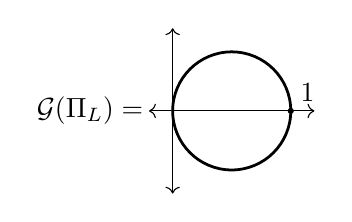
\begin{tikzpicture}[scale=1.5]
\draw(-0.7,0) node {$\cG(\proj_L)=$};
\draw [line width=1.0pt] (0.5,0) circle (0.5);
\draw [<->] (-.2,0) -- (1.2,0);
\draw [<->] (0,-.7) -- (0,.7);
\draw (1,0)  node [above right] {1};
\filldraw (1,0) circle ({0.6*1.5/1.5pt});
%\draw (0,1.2) node [above] {SRG of $\proj_{L}$};
\end{tikzpicture}
}
\raisebox{-.5\height}{
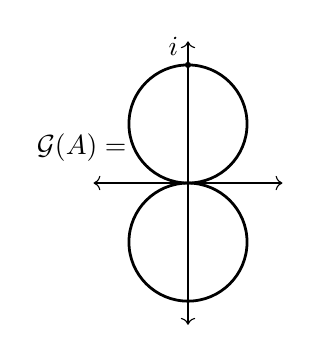
\begin{tikzpicture}[scale=1.5]
\draw(-0.9,0.3) node {$\cG(\opA)=$};
\draw [<->] (-.8,0) -- (.8,0);
\draw [<->] (0,-1.2) -- (0,1.2);
%\filldraw (0,1/2) circle ({0.6*1.5/1.5pt});
%\draw (0,1/2)   node [left] {$1/2$};
\filldraw (0,1) circle ({0.6*1.5/1.5pt});
\draw (0,1) node [above left] {$i$};
%\draw (-1pt,1) -- (1pt,1)   node [above left] {$1$};
%\draw (1.25,0) node [below] {$\frac{1}{2}$};
%\draw [decorate,decoration={brace,amplitude=4.5pt}](1.5,0) -- (1,0) ;
\draw [line width=1.0pt] (0,1/2) circle (1/2);
\draw [line width=1.0pt] (0,-1/2) circle (1/2);
\end{tikzpicture}
}
\raisebox{-.5\height}{
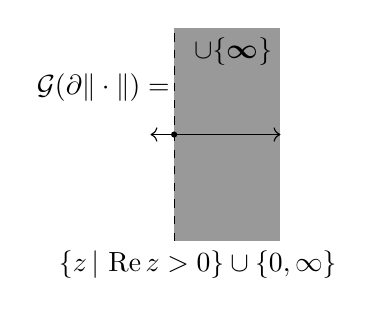
\begin{tikzpicture}[scale=1.5]
\draw(-0.6,0.4) node {$\cG(\partial \|\cdot\|)=$};
\draw(0.2,-1.1) node {$\{z \,|\,\Re z>0\}\cup\{0,\infty\}$};
\def\m{.9}
\fill [fill=medgrey] (0,{-\m})--(0,{\m})--({\m},{\m})--({\m},{-\m})--cycle;
\draw [<->] (-0.2,0) -- ({\m},0);
\draw [dashed] (0,{-\m}) -- (0,{\m});
\draw ({\m-0.4},{\m-0.2}) node {$\cup \{\binfty\}$};
\filldraw (0,0) circle ({0.6*1.5/1.5pt});
%\draw (-1pt,1) -- (1pt,1)   node [above left] {$1$};
%\draw (1.25,0) node [below] {$\frac{1}{2}$};
%\draw [decorate,decoration={brace,amplitude=4.5pt}](1.5,0) -- (1,0) ;
\end{tikzpicture}
}}}
\\
\mbox{
\raisebox{-.5\height}{
\!\!\!\!\!\!
\!\!\!\!\!\!
\raisebox{-.5\height}{
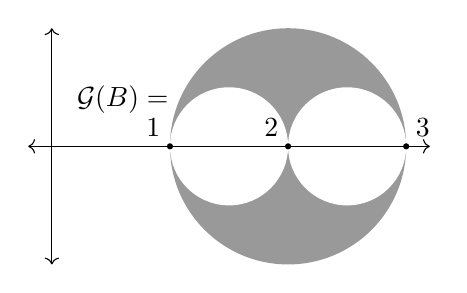
\begin{tikzpicture}[scale=1.5]
\draw(.6,0.4) node {$\cG(\opB)=$};
\fill [fill=medgrey] (2,0) circle (1);
\fill [fill=white] (1.5,0) circle (.5);
\fill [fill=white] (2.5,0) circle (.5);

\filldraw (1,0) circle ({0.6*1.5/1.5pt});
\draw (1,0)   node [above left] {$1$};
\filldraw (2,0) circle ({0.6*1.5/1.5pt});
\draw (2,0)   node [above left] {$2$};
\filldraw (3,0) circle ({0.6*1.5/1.5pt});
\draw (3,0)   node [above right] {$3$};
%\draw (1.25,0) node [below] {$\frac{1}{2}$};
%\draw [decorate,decoration={brace,amplitude=4.5pt}](1.5,0) -- (1,0) ;
\draw [<->] (-0.2,0) -- (3.2,0);
\draw [<->] (0,-1.) -- (0,1.);
\end{tikzpicture}}
}}
\end{center}
%\vspace{0.1in}

$\proj_L\colon\reals^2 \to \reals^2$ the projection onto a line $L$;
$\opA\colon\mathbb{R}^2 \to \mathbb{R}^2$ is $\opA(u,v) = (0,u)$;
 $\partial \|\cdot\|$ for $n\ge 2$;
and $\opB\colon\mathbb{R}^3\to\mathbb{R}^3$ is $\opB(u,v,w) = (u,2v,3w)$;
 Shapes obtained through direct calculations.

\end{frame}



\begin{frame}
\frametitle{SRG and eigenvalues}
For linear operators, SRG generalizes eigenvalues:\\
$\Lambda(\opA)\subseteq \cG(\opA)$, if $\opA\in \reals^{n\times n}$ and $n = 1$ or $n\ge 3$.
%where $\Lambda(\opA)$ denotes the set of eigenvalues of $\opA$.

\vspace{0.2in}
SRG of a $3\times 3$ matrix. The three points denote the eigenvalues.
\begin{center}
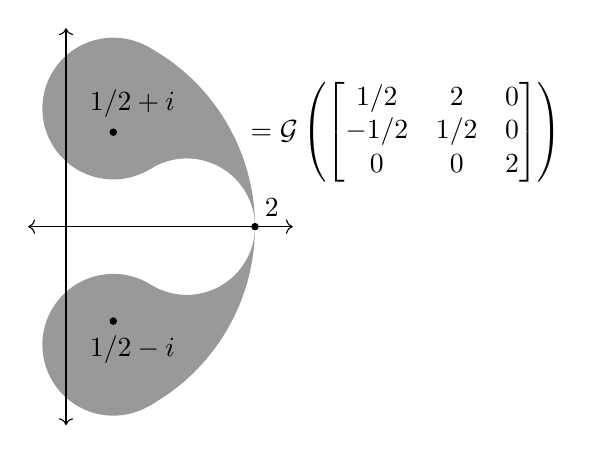
\begin{tikzpicture}[scale=1.2]
\def\a{1/2};
\def\b{2};
\def\c{1/2};
\fill [fill=medgrey] ({\a},{(\b+\c)/2}) circle ({(\b-\c)/2});

\def\x{0.896284298022351};
\def\y{0.613243566863332};
\def\u{0.852941212550304};
\def\v{1.911764686639837};

\fill[fill = medgrey] plot[line width=1.0pt, domain=0:{acos((-4 + \y^2 + 4 *\x - (\x)^2)/(4 + \y^2 - 4 *(\x) + (\x)^2))},variable=\p] ({( 2-(-4 + (\y)^2 + (\x)^2)/(2 *(-2 + (\x))) )*cos(\p)+(-4 + (\y)^2 + (\x)^2)/(2 *(-2 + (\x)))},{( 2-(-4 + (\y)^2 + (\x)^2)/(2 *(-2 + (\x))) )*sin(\p)}) --  plot[line width=1.0pt, domain={acos((-4 + \v^2 + 4 *\u - (\u)^2)/(4 + \v^2 - 4 *(\u) + (\u)^2)):0},variable=\p] ({( 2-(-4 + (\v)^2 + (\u)^2)/(2 *(-2 + (\u))) )*cos(\p)+(-4 + (\v)^2 + (\u)^2)/(2 *(-2 + (\u)))},{( 2-(-4 + (\v)^2 + (\u)^2)/(2 *(-2 + (\u))) )*sin(\p)});

\fill [fill=medgrey] ({\a},{-(\b+\c)/2}) circle ({(\b-\c)/2});

\def\x{0.896284298022351};
\def\y{0.613243566863332};
\def\u{0.852941212550304};
\def\v{1.911764686639837};

\fill[fill = medgrey] plot[line width=1.0pt, domain=0:{acos((-4 + \y^2 + 4 *\x - (\x)^2)/(4 + \y^2 - 4 *(\x) + (\x)^2))},variable=\p] ({( 2-(-4 + (\y)^2 + (\x)^2)/(2 *(-2 + (\x))) )*cos(\p)+(-4 + (\y)^2 + (\x)^2)/(2 *(-2 + (\x)))},{-( 2-(-4 + (\y)^2 + (\x)^2)/(2 *(-2 + (\x))) )*sin(\p)}) --  plot[line width=1.0pt, domain={acos((-4 + \v^2 + 4 *\u - (\u)^2)/(4 + \v^2 - 4 *(\u) + (\u)^2)):0},variable=\p] ({( 2-(-4 + (\v)^2 + (\u)^2)/(2 *(-2 + (\u))) )*cos(\p)+(-4 + (\v)^2 + (\u)^2)/(2 *(-2 + (\u)))},{-( 2-(-4 + (\v)^2 + (\u)^2)/(2 *(-2 + (\u))) )*sin(\p)});

\draw (0.15,1.05) node[above right]{$1/2+i$};
\draw (0.15,-1.05) node[below right]{$1/2-i$};
\draw (2,0) node[above right]{$2$};
\filldraw (1/2,1) circle (1.0/1.05pt);
\filldraw (1/2,-1) circle (1.0/1.05pt);
\filldraw (2,0) circle (1.0/1.05pt);

\draw (3.6,1) node[]{$=\cG\left(\begin{bmatrix}
1/2&2&0\\
-1/2&1/2&0\\
0&0&2
\end{bmatrix}\right)$};

\draw [<->] (-0.4,0) -- (2.4,0);
\draw [<->] (0,-2.1) -- (0,2.1);
\end{tikzpicture}
\end{center}
\end{frame}

\begin{frame}[plain]
\frametitle{Example: SRG of normal matrices}
For normal matrices, multiplicity of eigenvalues do not affect the SRG.
\vspace{-0.1in}

\raisebox{-.5\height}{
\!\!\!\!\!\!
\!\!\!\!\!\!
\!\!\!\!\!\!
\!\!\!\!\!\!
\!\!\!\!\!\!
\!\!\!\!\!\!
\!\!\!\!\!\!
\!\!\!\!\!\!
\mbox{
\raisebox{-.5\height}{
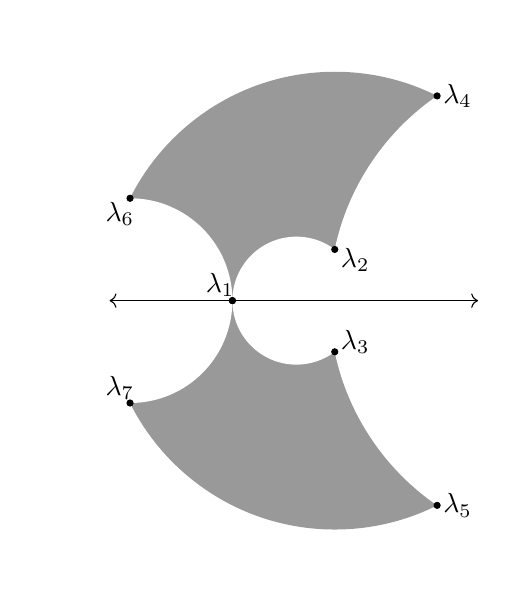
\begin{tikzpicture}[scale=1.3]
					\begin{scope}
						\clip (-1.25,-2.666666) rectangle (2.45,2.6666666);
						\fill[medgrey] (1,0) circle ({sqrt(5)});
						%\clip (-1.25,-2.3) rectangle (2.45,2.3);
					\end{scope}
					
					\fill[white] (5/8,0) circle (5/8);
					\fill[white] (-1,0) circle (1); 
					\begin{scope}
						\clip (-1.25,-2.3) rectangle (2.5,2.3);
						\fill[white] (27/8,0) circle ({sqrt((19/8)^2+(1/2)^2)}); 
					\end{scope}
					
					\filldraw (-1,1) circle (1.0/1.2pt);
					\filldraw (0,0) circle (1.0/1.2pt);
					\filldraw (1,0.5) circle (1.0/1.2pt);
					\filldraw (2,2) circle (1.0/1.2pt);
					
					\filldraw (-1,-1) circle (1.0/1.2pt);
					\filldraw (0,-0) circle (1.0/1.2pt);
					\filldraw (1,-0.5) circle (1.0/1.2pt);
					\filldraw (2,-2) circle (1.0/1.2pt);
					
					\draw (-1.1,0.85) node {$\lambda_6$};
					\draw (1.2,0.4) node {$\lambda_2$};
					\draw (2.2,2.0) node {$\lambda_4$};
					\draw (-1.1,-0.85) node {$\lambda_7$};
					\draw (1.2,-0.4) node {$\lambda_3$};
					\draw (2.2,-2.0) node {$\lambda_5$};
					\draw (-0.12,0.15) node {$\lambda_1$};
					
					\draw[<->] (-1.2,0) -- (2.4,0);					
				\end{tikzpicture}}
\raisebox{-.5\height}{
		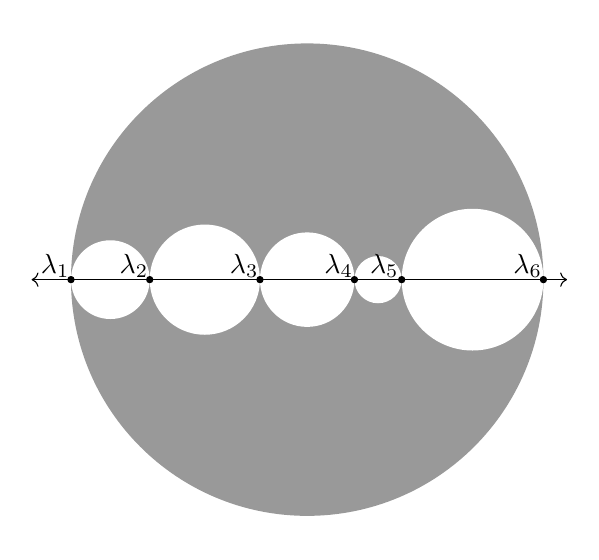
\begin{tikzpicture}[scale=1.0]
				\clip (-3.55,-3.2) rectangle (3.35,3.2);
				\draw (-3.2,0.18) node[] {$\lambda_1$};
				\fill[medgrey] (0,0) circle (3);
				%\draw (0,0) circle (3);
				
				\fill[white] (-2.5,0) circle (0.5);
				%\draw (-2.5,0) circle (0.5);
				\draw (-2.2,0.18) node[] {$\lambda_2$};
				
				
				\fill[white] (-1.3,0) circle (0.7);
				%\draw (-1.3,0) circle (0.7);
				\draw (-0.8,0.18) node[] {$\lambda_3$};
				
				
				\fill[white] (0,0) circle (0.6);
				%\draw (0,0) circle (0.6);
				\draw (0.4,0.18) node[] {$\lambda_4$};
				
				\fill[white] (0.9,0) circle (0.3);
				%\draw (0.9,0) circle (0.3);
				\draw (0.98,0.18) node[] {$\lambda_5$};
				
				\fill[white] (2.1,0) circle (0.9);
				%\draw (2.1,0) circle (0.9);
				\draw (2.8,0.18) node[] {$\lambda_6$};
				
				\filldraw (-3,0) circle ({1.0/0.9pt});
				\filldraw (-2,0) circle ({1.0/0.9pt});
				\filldraw (-0.6,0) circle ({1.0/0.9pt});
				\filldraw (0.6,0) circle ({1.0/0.9pt});
				\filldraw (1.2,0) circle ({1.0/0.9pt});
				\filldraw (3,0) circle ({1.0/0.9pt});
				
				
				\draw [<->] (-3.5,0) -- (3.3,0);
				% \draw [<->] (0,-3.2) -- (0,3.5);
				\end{tikzpicture}}
}}
\vspace{-0.15in}

(Left) SRG of an $n\times n$ normal matrix with one distinct real eigenvalue and three distinct complex conjugate eigenvalue pairs.
(Right) SRG of an $n\times n$ symmetric matrix with distinct eigenvalues $\lambda_1<\lambda_2<\dots<\lambda_6$.

\end{frame}


\begin{frame}
\frametitle{SRG of operator classes}
SRG of a collection of operators:
\[
\mathcal{G}(\cA)=\bigcup_{\opA\in \cA}\mathcal{G}(\opA).
\]
\vspace{0.2in}

%We focus more on SRGs of operator classes, rather than individual operators, because 
(Theorems are usually stated with operator classes.
For example, \\``If $\opA$ is $\beta/2$-cocoercive, i.e., if $\opA\in \cC_{\beta/2}$, then $\opI-\opA$ is nonexpansive.'')
% We now characterize the SRG of the Lipschitz, averaged, monotone, strongly monotone, and cocoercive operator classes.
\end{frame}





\begin{frame}[plain]
\setcounter{theorem}{18}
\begin{theorem}
\label{thm:monotone-srg}
Let $\mu,\beta,L\in (0,\infty)$ and $\theta\in(0,1)$.
Then
\vspace{-0.1in}
\begin{center}
\begin{tabular}{cc}
\raisebox{-.5\height}{
\begin{tikzpicture}[scale=1.5]
\draw (-1.1,0.5) node {$\cG(\cL_L)=$};
\fill[fill=medgrey] (0,0) circle (0.75);
%\draw[line width=1.0pt] (0,0) circle (0.75);
\draw [<->] (-1,0) -- (1,0);
\draw [<->] (0,-1) -- (0,1);
\draw (0.75,0) node [above right] {$L$};
\draw (-0.75,0) node [above left] {$-L$};
\filldraw (.75,0) circle ({0.6*1.5/1.5pt});
\filldraw (-.75,0) circle ({0.6*1.5/1.5pt});
\draw (0,-1.2) node  {$\left\{z\in \complex\,\big|\,|z|^2\le L^2\right\}$};
\end{tikzpicture}}
&
\raisebox{-.5\height}{
\begin{tikzpicture}[scale=1.5]
\draw (-0.85,0.5) node {$\cG(\cN_\theta)=$};
\fill[fill=medgrey] (0.25,0) circle (0.75);
\draw [<->] (-.8,0) -- (1.2,0);
\draw [<->] (0,-1) -- (0,1);
%\draw [dashed] (0,0) circle (1);
\draw (1,-0) node [above right] {$1$};
\draw (-0.5,-0) node [below] {$1-2\theta$};
\filldraw (1,0) circle ({0.6*1.5/1.5pt});
\filldraw (.25,0) circle ({0.6*1.5/1.5pt});
\filldraw (-.5,0) circle ({0.6*1.5/1.5pt});
\draw (0.625,0.1) node [above] {$\theta$};
\draw [decorate,decoration={brace,amplitude=4.5pt}] (0.25,0) -- (1,0) ;
\draw (0.4,-1.2) node  {$\left\{z\in \complex\,\big|\,|z|^2+(1-2\theta)\le 2(1-\theta)\Re z\right\}$};
\end{tikzpicture}}
\end{tabular}
\end{center}
\raisebox{-.5\height}{
\!\!\!\!\!\!\!\!\!\!\!\!
\!\!\!\!\!\!\!\!\!\!
\begin{tabular}{ccc}
\raisebox{-.5\height}{
\begin{tikzpicture}[scale=1.5]
\draw (-0.5,0.5) node {$\cG(\cM)=$};
\fill[fill=medgrey] (0,-1) rectangle (1,1);
\draw [<->] (-0.2,0) -- (1,0);
\draw [<->] (0,-1) -- (0,1);
%\draw [line width=1.0pt] (0,-1.2) -- (0,1.2);
%\draw (1,-1pt) -- (1,1pt)   node [above] {$1$};
\draw (0.7,.85) node {$\cup \{\binfty\}$};
\draw (0.4,-1.2) node {$\left\{z\in \complex\,|\,\Re z\ge 0\right\}\cup\{\infty\}$};
\end{tikzpicture}}
&
\!\!\!\!\!\!\!\!\!\!\!\!
\raisebox{-.5\height}{
\begin{tikzpicture}[scale=1.5]
\draw [<->] (0,-1) -- (0,1);

\draw (-0.2,0.5) node [fill=white] {$\cG(\cM_\mu)=$};
\fill[fill=medgrey] (0.3,-1) rectangle (1,1);

\draw [<->] (-0.2,0) -- (1,0);

%\draw [line width=1.0pt] (0.5,-1.2) -- (0.5,1.2);
%\draw (1,-1pt) -- (1,1pt)   node [above] {$1$};
\draw (0.7,.85) node {$\cup \{\binfty\}$};
\filldraw (.3,0) circle ({0.6*1.5/1.5pt});
\draw (0.3,0) node [above left] {$\mu$};
\draw (0.4,-1.2) node {$\left\{z\in \complex\,|\,\Re z\ge \mu\right\}\cup\{\infty\}$};

\end{tikzpicture}}
&
\!\!\!\!\!\!\!\!\!\!\!\!\!\!
\raisebox{-.5\height}{
\begin{tikzpicture}[scale=1.5]
\draw (-0.45,0.3) node {$\cG(\cC_\beta)=$};
\fill[fill=medgrey] (0.6,0) circle (0.6);
%\draw[line width=1.0pt] (0.5,0) circle (0.5);
\draw [<->] (-0.5,0) -- (1.5,0);
\draw [<->] (0,-.8) -- (0,.8);
\filldraw (1.2,0) circle ({0.6*1.5/1.5pt});
\draw (1.2,0) node [above right] {\!$1/\beta$};
\draw (0.4,-1) node  {$\left\{z\in \complex\,\big|\,\Re z\ge \beta|z|^2\right\}$};
\end{tikzpicture}}
\end{tabular}
}
\end{theorem}
\end{frame}



\begin{frame}
\frametitle{SRG of subdifferential operators}
\begin{theorem}
\label{thm:cvx-srg-first}
Let $0<\mu<L<\infty$. Then
%Let $\partial \mathcal{F}_{0,\infty}$ be the class of subdifferential operators of CCP functions. Then
\begin{center}
\begin{tabular}{cc}
\!\!\!\!\!\!
\raisebox{-.5\height}{
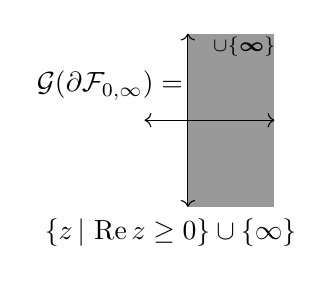
\begin{tikzpicture}[scale=1.1]
\draw (-0.9,0.4) node {$\cG(\partial \mathcal{F}_{0,\infty})=$};
\fill[fill=medgrey] (0,-1) rectangle (1,1);
\draw [<->] (-0.5,0) -- (1,0);
\draw [<->] (0,-1) -- (0,1);
%\draw [line width=1.0pt] (0,-1.2) -- (0,1.2);
%\draw (1,-1pt) -- (1,1pt)   node [above] {$1$};
\draw (0.65,.85) node {$\scriptstyle\cup \{\binfty\}$};
\draw (-0.2,-1.3) node {$\left\{z\,|\,\Re z\ge 0\right\}\cup\{\infty\}$};
\end{tikzpicture}}
&\!\!\!\!\!\!\!\!\!\!\!\!\!\!\!
\raisebox{-.5\height}{
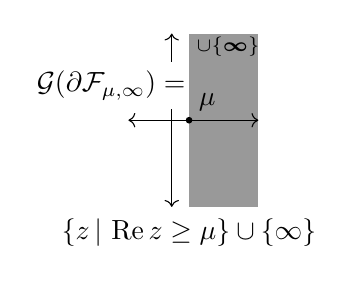
\begin{tikzpicture}[scale=1.1]
\draw [<->] (0,-1) -- (0,1);
\draw (-0.7,0.4)  node [fill=white]{$\cG(\partial \mathcal{F}_{\mu,\infty})=$};
\fill[fill=medgrey] (0.2,-1) rectangle (1,1);
\draw [<->] (-0.5,0) -- (1,0);
%\draw [line width=1.0pt] (0.5,-1.2) -- (0.5,1.2);
%\draw (1,-1pt) -- (1,1pt)   node [above] {$1$};
\draw (0.65,.85) node {$\scriptstyle \cup \{\binfty\}$};
\draw (0.2,0pt) node [above right] {$\mu$};
\filldraw (.2,0) circle ({0.6*1.5/1pt});
\draw (0.2,-1.3) node{$\left\{z\,|\,\Re z\ge \mu\right\}\cup\{\infty\}$};
\end{tikzpicture}}
\end{tabular}\\
\vspace{0.1in}
\begin{tabular}{cc}
\raisebox{-.5\height}{
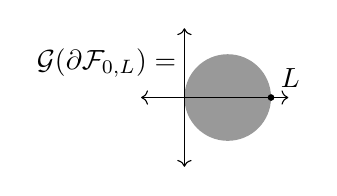
\begin{tikzpicture}[scale=1.1]
\draw (-0.9,0.4) node {$\cG(\partial \mathcal{F}_{0,L})=$};
\fill[fill=medgrey] (0.5,0) circle (0.5);
%\draw[line width=1.0pt] (0.5,0) circle (0.5);
\draw [<->] (-0.5,0) -- (1.2,0);
\draw [<->] (0,-.8) -- (0,.8);
\draw (1,0) node [above right] {$L$};
\filldraw (1,0) circle ({0.6*1.5/1pt});
%\draw (0.,-1) node {$\left\{z\,|\,|z|^2\le L\Re z\right\}$};
\end{tikzpicture}}
&\!\!\!\!\!\!\!\!\!\!\!\!
\raisebox{-.5\height}{
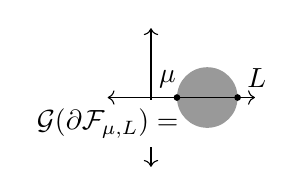
\begin{tikzpicture}[scale=1.1]
\draw [<->] (0,-.8) -- (0,.8);
\draw (-0.5,-0.3)  node [fill=white] {$\cG(\partial \mathcal{F}_{\mu,L})=$};
\fill[fill=medgrey] (0.65,0) circle (0.35);
%\draw[line width=1.0pt] (0.65,0) circle (0.35);
\draw [<->] (-0.5,0)-- (1.2,0);
\filldraw (1,0) circle ({0.6*1.5/1pt});
\draw (1,0pt) node [above right] {$L$};
\filldraw (.3,0) circle ({0.6*1.5/1pt});
\draw (0.4,0pt) node [above left] {$\mu$};
%\draw (0.,-1) node {$\left\{z \,|\,|z|^2+\mu L\le(L+\mu)\Re z\right\}$};
\end{tikzpicture}
}
\end{tabular}
\end{center}
\vspace{-0.1in}
\end{theorem}
\end{frame}






\begin{frame}
\frametitle{SRG-full classes} 
An operator defines its SRG.
Conversely, can we examine the SRG and conclude something about the operator?
%To perform this type of reasoning, we need further conditions.

\vspace{0.2in}

A class of operators $\cA$ is \emph{SRG-full} if
%
\[
\opA\in \cA
\quad\Leftrightarrow\quad
\cG(\opA)\subseteq\cG(\cA).
\]
%
Since $\opA\in \cA\Rightarrow\cG(\opA)\subseteq \cG(\cA)$ holds by definition, $\cG(\opA)\subseteq \cG(\cA)\Rightarrow \opA\in \cA$ is the substance of SRG-fullness.

\vspace{0.2in}

Essentially, a class is SRG-full if it can be fully characterized by its SRG;
we can check membership $\opA\in \cA$ by verifying (through geometric arguments) containment $\cG(\opA)\subseteq \cG(\cA)$ in the 2D plane. 


\end{frame}


\begin{frame}
\frametitle{SRG-full classes} 
SRG-fullness assumes the desirable property $\cG(\opA)\subseteq \cG(\cA)\Rightarrow \opA\in \cA$.
The following characterizes classes with this property.
\begin{theorem} \label{thm:srg-full}
%%%%%%%%%%%%%%%%%%%%%%%%%%%%%%%%%%%%%%%%
An operator class $\cA$ is SRG-full if it is defined by
\[
\opA\in \cA\quad\Leftrightarrow\quad
h\left(\|u-v\|^2,\|x-y\|^2,\langle u-v,x-y\rangle\right)\le 0,
\quad \forall u\in \opA x,\,v\in \opA y
\]
for some nonnegative homogeneous function $h\colon\reals^3\rightarrow\reals$.
\end{theorem}

\vspace{0.2in}

$h$ is nonnegative homogeneous if $\theta h(a,b,c)= h(\theta a,\theta b,\theta c)$ for all $\theta\ge 0$. (We do not assume $h$ is smooth.)

\end{frame}


\begin{frame}
\frametitle{Example: SRG-full classes} 
When a class $\cA$ is defined by $h$ as in  Theorem~\ref{thm:srg-full}, we say $h$ \emph{represents} $\cA$.
\vspace{0.2in}

$\mu$-strongly monotone class $\cM_\mu$ represented by $h(a,b,c)=\mu b-c$:
\[
\opA\in \cM_{\mu}
\quad\Leftrightarrow\quad
\mu\|x-y\|^2\le \langle u-v,x-y\rangle,\quad\forall u\in \opA x,\,v\in \opA y.
\]
\vspace{0.2in}

Firmly nonexpansive class $\cN_{1/2}$ represented by $h(a,b,c)=a-c$:
\[
\opA\in \cN_{1/2}
\quad\Leftrightarrow\quad
\|u-v\|^2\le \langle u-v,x-y\rangle,\quad\forall u\in \opA x,\,v\in \opA y.
\]

\vspace{0.2in}
By Theorem~\ref{thm:srg-full}, $\cM$, $\cM_\mu$, $\cC_\beta$, $\cL_L$, and $\cN_\theta$ are all SRG-full.

\end{frame}



\begin{frame}
\frametitle{Example: Class of subdifferentials are not SRG-full}
Classes $\partial \cF_{0,\infty}$, $\partial \cF_{\mu,\infty}$, $\partial \cF_{0,L}$, and $\partial \cF_{\mu,L}$ are \emph{not} SRG-full.

\vspace{0.2in}

For example, 
\[
\opA(z_1,z_2)=
\begin{bmatrix}
0&-1\\
1&0
\end{bmatrix}
\begin{bmatrix}
z_2\\z_2
\end{bmatrix}
\]
satisfies $\cG(\opA)=\{-i,i\}\subseteq \cG( \partial \cF_{0,\infty})$, but
$\opA\notin \partial \cF_{0,\infty}$.

\vspace{0.2in}
(If $\nabla f=\opA$ for a function $f$, then $D\opA=\nabla^2f$ must be symmetric.)
\end{frame}

\begin{frame}
\frametitle{Role of maximality}
Maximality is mostly orthogonal to the notion of the SRG:
non-maximal operators have a well-defined SRGs, and SRG-full classes contain non-maximal operators.
\vspace{0.2in}

This separation allows the geometric analyses via SRGs being entangled with the subtleties of maximality.
\end{frame}




\section{Operator and SRG transformations}
%\begin{frame}
%% In this section, we present Theorems~\ref{thm:srg-scaling-translation} and \ref{thm:srg-inversion}, which describe how certain transformations of operators map to changes in their SRGs.
%In this section, we show how transformations of operators map to changes in their SRGs and analyze convergence of various fixed-point iterations.
%\end{frame}




\begin{frame}
\frametitle{Intersection}
%%%%%%%%%%%%%%%%%%%%%%%%%%%%%%%%%%%%%%%%
\begin{theorem} \label{thm:srg-intersection}
%%%%%%%%%%%%%%%%%%%%%%%%%%%%%%%%%%%%%%%%
If $\cA$ and $\cB$ are SRG-full classes, then  $\cA\cap \cB$ is SRG-full, and
\[
\cG(\cA\cap \mathcal{B})=\cG(\cA)\cap \cG(\mathcal{B}).
\]
\end{theorem}

\vspace{0.2in}

The substance of Theorem~\ref{thm:srg-intersection} is $\cG(\cA\cap \mathcal{B})\supseteq\cG(\cA)\cap \cG(\mathcal{B})$ since $\cG(\cA\cap \mathcal{B})\subseteq \cG(\cA)\cap \cG(\mathcal{B})$ holds by definition, regardless of SRG-fullness.
\end{frame}




\begin{frame}
\frametitle{Example: Non-SRG-full example}
Theorem~\ref{thm:srg-intersection} does not apply when the operator classes are not SRG-full.
For example, although
\[
\partial \cF_{\mu,L}=\partial \cF_{\mu,\infty}\cap \partial \cF_{0,L}
\]
we have the strict containment
\begin{center}
\begin{tabular}{lll}
\raisebox{-.5\height}{
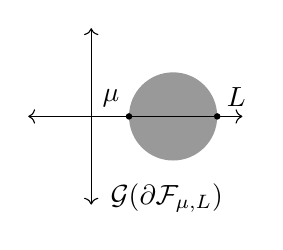
\begin{tikzpicture}[scale=1.6]
\fill[fill=medgrey] (0.65,0) circle (0.35);
\draw [<->] (-0.5,0)-- (1.2,0);
\draw [<->] (0,-.7) -- (0,.7);
\filldraw (1,0) circle ({0.6*1.5/1.5pt});
\draw (1,0pt) node [above right] {$L$};
\filldraw (.3,0) circle ({0.6*1.5/1.5pt});
\draw (0.3,0pt) node [above left] {$\mu$};
\draw (0.6,-.65) node {$\cG(\partial \mathcal{F}_{\mu,L})$};
\end{tikzpicture}
}
&$\subset$ &
\raisebox{-.5\height}{
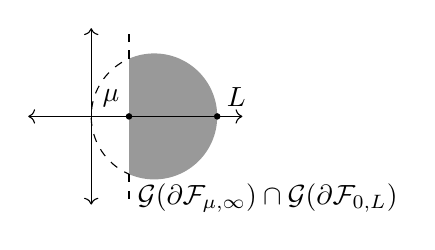
\begin{tikzpicture}[scale=1.6]
\begin{scope}
\clip (0.3,-.7) rectangle (1.2,.7);
\fill[fill=medgrey] (0.5,0) circle (0.5);
\end{scope}
\begin{scope}
\clip (0.3,-.7) rectangle (-0.5,.7);
\draw[dashed] (0.5,0) circle (0.5);
\end{scope}
\draw[dashed] (0.3,0.458258) -- (0.3,0.7);
\draw[dashed] (0.3,-0.458258) -- (0.3,-0.7);
\draw [<->] (-0.5,0) -- (1.2,0);
\draw [<->] (0,-.7) -- (0,.7);

\draw (0.3,0pt) node [above left] {$\mu$};
\filldraw (.3,0) circle ({0.6*1.5/1.5pt});
\draw (1.4,-.65) node{$\cG(\partial \mathcal{F}_{\mu,\infty})\cap \cG(\partial \mathcal{F}_{0,L})$};
\draw (1,0) node [above right] {$L$};
\filldraw (1,0) circle ({0.6*1.5/1.5pt});
\end{tikzpicture}}
\end{tabular}
\end{center}
% \[
% \cG(\partial \cF_{\mu,L})\subset 
% \cG(\partial \cF_{\mu,\infty})\cap\cG( \partial \cF_{0,L})
% \quad\text{ (strict inclusion).}
% \]
\end{frame}


\begin{frame}
\frametitle{Scaling and translation}
\begin{theorem}
%\emph{Scaling and translation.}
\label{thm:srg-scaling-translation}
Let $\alpha\in \reals$ and $\alpha\ne 0$.
If $\cA$ is a class of operators, then 
\[
\cG(\alpha \cA)=\alpha\cG(\cA),\qquad\cG(\opI+ \cA)=1+\cG(\cA).
\]
If $\cA$ is furthermore SRG-full, then $\alpha \cA$ and $\opI+ \cA$ are SRG-full.
\end{theorem}

\vspace{0.4in}

Note a class of operators can consist of a single operator. So
\[
\cG(\alpha \opA)=\alpha\cG(\opA),\qquad\cG(\opI+ \opA)=1+\cG(\opA)
\]
\end{frame}



\begin{frame}
\frametitle{Convergence analysis: gradient descent}
Consider
\[
\begin{array}{ll}
\underset{x\in \reals^n}{\mbox{minimize}}& f(x),
\end{array}
\]
where $f$ is $\mu$-strongly convex and $L$-smooth with $0<\mu<L<\infty$.
\vspace{0.2in}

Gradient descent
\[
x^{k+1}=x^k-\alpha \nabla f(x^k)
\]
converges with rate
\[
\|x^k-x^\star\|\le
\left(\max\{|1-\alpha\mu|,|1-\alpha L|\}\right)^k
\|x^0-x^\star\|
\]
for $\alpha\in (0,2/L)$
by the following Proposition~\ref{fact:forward-step}.
\end{frame}



\begin{frame}[plain]
\frametitle{Convergence analysis: gradient descent}

%%%%%%%%%%%%%%%%%%%%%%%%%%%%%%%%%%%%%%%%
\setcounter{proposition}{1}

\begin{proposition} \label{fact:forward-step}
%%%%%%%%%%%%%%%%%%%%%%%%%%%%%%%%%%%%%%%%
%If $f\in \mathcal{F}_{\mu,L}$,then 
Let $0<\mu<L<\infty$ and $\alpha\in (0,\infty)$.
If $\cA= \partial \cF_{\mu,L}$, then
$\opI-\alpha\cA\subseteq \cL_R$
for 
\[
R= \max\{|1-\alpha\mu|,|1-\alpha L|\}.
\]
Result is tight in the sense that $\opI-\alpha\cA\nsubseteq \cL_R$ for any smaller value of $R$.
% If $f\in \cF_{\mu,L}$, then 
% \[
% I-\alpha \nabla f\in  \cL\left({\max\{|1-\alpha\mu|,|1-\alpha L|\}}\right).
% \]
\end{proposition}
%Proposition~\ref{fact:forward-step} proves the gradient method $x^{k+1}=x^k-\alpha \nabla f(x^k)$ converges linearly at the rate $\cO(R^k)$ when $f$ is $\mu$-strongly convex, $\nabla f$ is $L$-Lipschitz, and $\alpha\in (0,2/L)$.
\textbf{Proof.}
By Theorems~\ref{thm:cvx-srg-first} and \ref{thm:srg-scaling-translation}, we have the geometry
\begin{center}
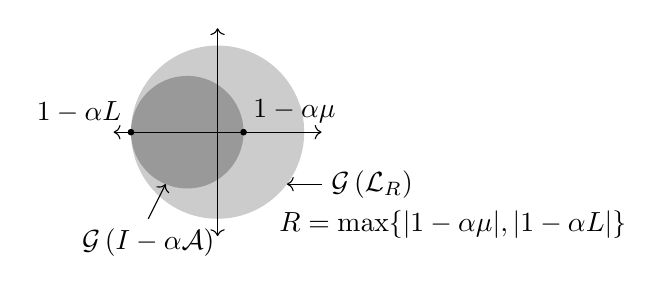
\begin{tikzpicture}[scale=1.1]
\def\x{-0.6};
\def\w{0.8};
\fill [fill=lightgrey] (0,0) circle (1);

\fill[fill=medgrey] (-0.35,0) circle (0.65);
%\draw[line width=1.0pt] (-0.35,0) circle (0.65);
\draw [<->] (-1.2,0) -- (1.2,0);
\draw [<->] (0,-1.2) -- (0,1.2);
\draw (-1,0)node [above left] {$1-\alpha L$};
\filldraw (-1,0) circle ({0.6*1.5/1pt});
\filldraw (.3,0) circle ({0.6*1.5/1pt});
\draw (0.3,0) node [above right] {$1-\alpha \mu$};
\draw[->] (-0.8,-1.)--(\x,{-sqrt(3-7*\x-10*((\x)^2))/sqrt(10)});
%\draw (-0.8,-1.) node [below] {$\cG\left(I-\alpha \partial \mathcal{F}_{\mu,L}\right)$};
\draw (-0.8,-1.) node [below] {$\cG\left(\opI-\alpha \cA\right)$};
\draw[->] (1.2,-.6)--(\w,{-sqrt(1-\w^2)});
\draw (1.2,-.6) node [right] {$\cG\left(\cL_R\right)$};
\draw (.6,-.8) node [below right] {$R={\max\{|1-\alpha\mu|,|1-\alpha L|\}}$};
\end{tikzpicture}
\end{center}
The containment of $\cG(\opI-\alpha\cA)$ holds for $R$ and fails for smaller $R$.
Since $\cL_R$ is SRG-full by Theorem~\ref{thm:srg-full}, the containment of the SRG in $\ecomplex$ equivalent to the containment of the class.
% Since $\cL\left({\max\{|1-\alpha\mu|,|1-\alpha L|\}}\right)$ is SRG-representable, 
% the inclusion of the SRG in $\ecomplex$ implies the inclusion of the class by Theorem~\ref{thm:srg-representation}.
\qed
\end{frame}


\begin{frame}
\frametitle{Convergence analysis: Forward step method}
Consider
\[
\begin{array}{ll}
\underset{x\in \reals^n}{\mbox{find}}&0\in \opA x,
\end{array}
\]
where $\opA\colon\reals^n\rightarrow\reals^n$.
Consider the forward step method
\[
x^{k+1}=x^k-\alpha \opA x^k
\]
under the following two setups.

\vspace{0.2in}

If $\opA$ is $\mu$-strongly monotone and $L$-Lipschitz with $0<\mu<L<\infty$,
\[
\|x^k-x^\star\|\le
\left(1-2\alpha\mu+\alpha^2 L^2\right)^{k/2}
\|x^0-x^\star\|
\]
for $\alpha\in (0,2\mu/L^2)$ by Proposition~\ref{thm:cont-sm-Lipschitz}.
\end{frame}





\begin{frame}
\begin{proposition}
\label{thm:cont-sm-Lipschitz}
Let $0<\mu<L<\infty$ and $\alpha\in (0,\infty)$.
If $\cA=\mathcal{M}_\mu\cap \mathcal{L}_L$,
then $\opI-\alpha \cA\subseteq \cL_R$
for
\[
R= \sqrt{1-2\alpha\mu+\alpha^2 L^2}.
\]
Result is tight in the sense that $\opI-\alpha\cA\nsubseteq \cL_R$ for any smaller value of $R$.
% If $A\in \mathcal{M}_\mu\cap \mathcal{L}_L$,
% then $I-\alpha A\in \cL\left(\sqrt{1-2\alpha\mu+\alpha^2 L^2}\right)$.
\end{proposition}
\end{frame}
% Proposition~\ref{thm:cont-sm-Lipschitz} proves the ``forward-step method'' $x^{k+1}=x^k-\alpha Ax^k$ converges linearly at the rate $\cO(R^k)$ if $A$ is $\mu$-strongly monotone, $L$-Lipschitz, and $\alpha\in (0,2\mu/L^2)$.



\begin{frame}[plain]
\textbf{Proof.}
First consider the case $\alpha\mu>1$.
By Theorems~\ref{thm:monotone-srg} and \ref{thm:srg-scaling-translation}, we have
\raisebox{-.5\height}{
\!\!\!\!\!\!\!\!\!\!\!\!\!\!\!\!\!\!\!\!\!
\begin{tabular}{ccc}
\raisebox{-.5\height}{
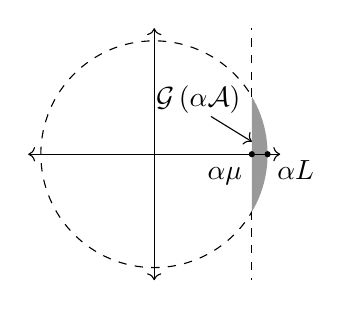
\begin{tikzpicture}[scale=.8]
\def\m{1.55};
\def\L{1.8};

\begin{scope}
\clip (\m,-2) rectangle (2,2);
\fill[fill=medgrey] (0,0) circle (\L);
\end{scope}

\begin{scope}
\clip (-2,-2) rectangle (\m,2);
\draw[dashed] (0,0) circle (\L);
\end{scope}

\draw[dashed] (\m,{sqrt(\L^2-\m^2)})--(\m,2);
\draw[dashed] (\m,-{sqrt(\L^2-\m^2)})--(\m,-2);

\draw [<->] (0,-2) -- (0,2);
\draw [<->] (-2,0) -- (2,0);
\filldraw (\m,-0.0) circle ({0.6*1.5/.8pt});
\draw (\m,-0.05) node [below left] {$\alpha \mu$};
\filldraw (\L,0.0) circle ({0.6*1.5/.8pt});
\draw (\L,0.05) node [below right] {$\alpha L$};


\draw[->] (.9,.6)--(\m,.2);
\draw (.7,.5) node [above] {$\cG\left(\alpha\cA\right)$};
\end{tikzpicture}
}
&
\!\!\!\!\!\!\!\!\!\!\!\!\!
\raisebox{-.5\height}{
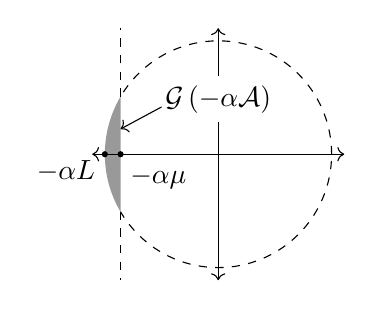
\begin{tikzpicture}[scale=.8]
\def\m{1.55};
\def\L{1.8};

\begin{scope}
\clip ({-\m},-2) rectangle (-2,2);
\fill[fill=medgrey] (0,0) circle (\L);
\end{scope}

\begin{scope}
\clip (2,-2) rectangle ({-\m},2);
\draw[dashed] (0,0) circle (\L);
\end{scope}

\draw[dashed] ({-\m},{sqrt(\L^2-\m^2)})--({-\m},2);
\draw[dashed] ({-\m},-{sqrt(\L^2-\m^2)})--({-\m},-2);

\draw [<->] (0,-2) -- (0,2);
\draw [<->] (-2,0) -- (2,0);
\filldraw ({-\m},-0.0) circle ({0.6*1.5/.8pt});
\draw ({-\m},-0.05) node [below right] {$-\alpha \mu$};
\filldraw ({-\L},0.0) circle ({0.6*1.5/.8pt});
\draw ({-\L},0.05) node [below left] {$-\alpha L$};

\draw (0,.5) node [above, fill=white] {$\cG\left(-\alpha\cA\right)$};
\draw[->] (-.9,.75)--({-\m},.4);
\end{tikzpicture}
}
&
\!\!\!\!\!\!\!\!\!\!\!\!\!
\raisebox{-.5\height}{
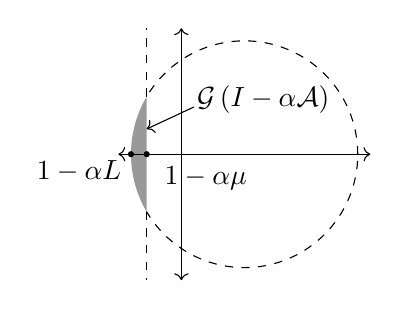
\begin{tikzpicture}[scale=.8]
\def\m{1.55};
\def\L{1.8};

\begin{scope}
\clip ({1-\m},-2) rectangle (-1,2);
\fill[fill=medgrey] (1,0) circle (\L);
\end{scope}

\begin{scope}
\clip (3.0,-2) rectangle ({1-\m},2);
\draw[dashed] (1,0) circle (\L);
\end{scope}

\draw[dashed] ({1-\m},{sqrt(\L^2-\m^2)})--({1-\m},2);
\draw[dashed] ({1-\m},-{sqrt(\L^2-\m^2)})--({1-\m},-2);

\draw [<->] (0,-2) -- (0,2);
\draw [<->] (-1,0) -- (3.0,0);
\filldraw ({1-\m},-0.0) circle ({0.6*1.5/.8pt});
\draw ({1-\m+0.13},-0.05) node [below right] {$1-\alpha \mu$};
\filldraw ({1-\L},0.0) circle ({0.6*1.5/.8pt});
\draw ({1-\L},0.05) node [below left] {$1-\alpha L$};

\draw[->] (0.2,.75)--({1-\m},.4);
\draw (1.3,.5) node [above] {$\cG\left(\opI-\alpha\cA\right)$};
\end{tikzpicture}
}
\end{tabular}
}
\raisebox{-.5\height}{
\!\!\!\!\!\!\!\!\!\!\!\!\!\!\!\!\!\!\!\!\!
\begin{tabular}{cc}
\raisebox{-.5\height}{
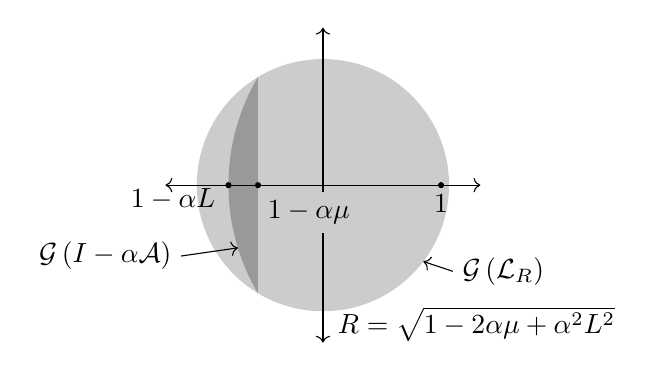
\begin{tikzpicture}[scale=1.5]
\clip (-2.5,-1.333333) rectangle (2.5,1.333333);
\def\m{1.55};
\def\L{1.8};
\fill[fill=lightgrey] (0,0) circle ({sqrt(1-2*\m+\L^2)});


\begin{scope}
\clip ({1-\m},-1.333333) rectangle (-1.3333333,1.333333);
\fill[fill=medgrey] (1,0) circle (\L);
\end{scope}
%\begin{scope}
%\clip ({1-\m},-1.5) rectangle (2.5,1.5);
%\draw [dashed] (1,0) circle (\L);
%\end{scope}
%\draw[line width=1.0pt] (0.35,0) circle (1);
%\draw [dashed] (0,0) circle (.35);
%\draw [line width=1.0pt] (-.35,-0.714143) -- (-.35,0.714143);
\draw [<->] (-1.33333333,0) -- (1.333333333,0);
\draw [<->] (0,{-2/1.5}) -- (0,{2/1.5});
%\draw [dashed] ({1-\m},{sqrt(\L^2-\m^2)}) -- (0,{sqrt(\L^2-\m^2)});
\filldraw ({1-\m},-0.0) circle ({0.6*1.5/1.5pt});
\draw ({1-\m},-0.05) node [below right, fill=lightgrey] {$1-\alpha \mu$};
\filldraw ({1-\L},0.0) circle ({0.6*1.5/1.5pt});
\draw ({1-\L-0.03},0.05) node [below left] {$1-\alpha L$};
\filldraw (1,0) circle ({0.6*1.5/1.5pt})  node [below] {$1$};
%\filldraw (0,{sqrt(\L^2-\m^2)}) circle ({0.6*1.5/1.5pt}) node [below right] {$\alpha\sqrt{L^2-\mu^2}$} ;
%\filldraw (0,{sqrt(1-2*\m+\L^2)}) circle ({0.6*1.5/1.5pt}) node [above right] {$\sqrt{1-2\alpha\mu+\alpha^2 L^2}$};
%\coordinate (I1) at (1,0);
%\coordinate (I2) at ({1-\m},0);
%\coordinate (I3) at ({1-\m},{sqrt(\L^2-\m^2)});
%\draw [] (I1)-- (I3);
%\tkzMarkRightAngle[size=.053](I1,I2,I3);

\def\w{-.72};

\draw[->] (-1.2,-.6)--(\w,{-sqrt(\L^2-(\w-1)^2)});
\draw (-1.2,-.6) node [left] {$\cG\left(\opI-\alpha\cA\right)$};

\def\y{.85};
\draw[->] (1.1,-.73)--(\y,{-sqrt(1-2*\m+\L^2-\y^2)});
\draw (1.1,-.73) node [right] {$\cG\left(\cL_R\right)$};
\draw (1.3,-.95) node [below] {$R=\sqrt{1-2\alpha\mu+\alpha^2 L^2}$};
\end{tikzpicture}
}
&\!\!\!\!\!\!\!\!\!\!\!\!\!\!\!
\raisebox{-.5\height}{
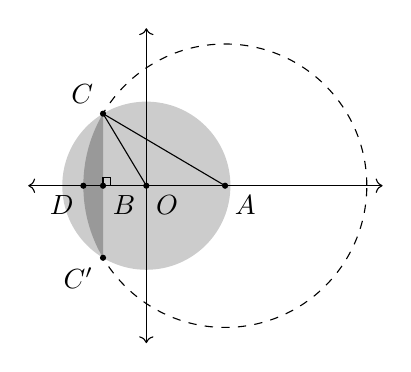
\begin{tikzpicture}[scale=1]
\def\m{1.55};
\def\L{1.8};
\fill[fill=lightgrey] (0,0) circle ({sqrt(1-2*\m+\L^2)});

\begin{scope}
\clip ({1-\m},-1.5) rectangle (-1.5,1.5);
\fill[fill=medgrey] (1,0) circle (\L);
\end{scope}
\begin{scope}
\clip ({1-\m},-2) rectangle (3,2);
\draw[dashed] (1,0) circle (\L);
\end{scope}
%\begin{scope}
%\clip ({1-\m},-1.5) rectangle (2.5,1.5);
%\draw [dashed] (1,0) circle (\L);
%\end{scope}
%\draw[line width=1.0pt] (0.35,0) circle (1);
%\draw [dashed] (0,0) circle (.35);
%\draw [line width=1.0pt] (-.35,-0.714143) -- (-.35,0.714143);
\draw [<->] (-1.5,0) -- (3,0);
\draw [<->] (0,-2) -- (0,2);
%\draw [dashed] ({1-\m},{sqrt(\L^2-\m^2)}) -- (0,{sqrt(\L^2-\m^2)});
%\filldraw ({1-\m},0) circle ({0.6*1.5/1pt}) node [below right] {$1-\alpha \mu$};
%\filldraw ({1-\L},0) circle ({0.6*1.5/1pt}) node [below left] {$1-\alpha L$};
%\filldraw (0,{sqrt(\L^2-\m^2)}) circle ({0.6*1.5/1pt}) node [below right] {$\alpha\sqrt{L^2-\mu^2}$} ;
%\filldraw (0,{sqrt(1-2*\m+\L^2)}) circle ({0.6*1.5/1pt}) node [above right] {$\sqrt{1-2\alpha\mu+\alpha^2 L^2}$};
\coordinate (I1) at (1,0);
\coordinate (I2) at ({1-\m},0);
\coordinate (I3) at ({1-\m},{sqrt(\L^2-\m^2)});
\coordinate (I4) at ({1-\m},{-sqrt(\L^2-\m^2)});
\coordinate (I5) at ({1-\L},0);
\draw [] (I1)-- (I3);
\tkzMarkRightAngle[size=.1](I1,I2,I3);
\draw (I1) node[below right] {$A$};
\draw (I2) node[below right] {$B$};
\draw (I3) node[above left] {$C$};
\draw (I4) node[below left] {$C'$};
\draw (I5) node[below left] {$D$};
\filldraw (I1) circle ({0.6*1.5/1pt});
\filldraw (I2) circle ({0.6*1.5/1pt});
\filldraw (I3) circle ({0.6*1.5/1pt});
\filldraw (I4) circle ({0.6*1.5/1pt});
\filldraw (I5) circle ({0.6*1.5/1pt});
\filldraw (0,0) circle ({0.6*1.5/1pt});
\draw (0,0) node[below right] {$O$};
\draw [] (0,0)-- (I3);

%
%
%\def\w{-.72};
%
%\draw[->] (-1.5,-.6)--(\w,{-sqrt(\L^2-(\w-1)^2)});
%\draw (-1.5,-.6) node [left] {$\cG\left(I-\alpha(\cM_\mu\cap \cL_L)\right)$};
%
%\def\y{.85};
%\draw[->] (1.1,-.73)--(\y,{-sqrt(1-2*\m+\L^2-\y^2)});
%\draw (1.1,-.73) node [right] {$\cG\left(\cL\left(\sqrt{1-2\alpha\mu+\alpha^2 L^2}\right)\right)$};

\end{tikzpicture}
}
\end{tabular}
}
To clarify, $O$ is the center of the circle with radius $\overline{OC}$ (lighter shade) and $A$ is the center of the circle with radius $\overline{AC}=\overline{AD}$ defining the inner region (darker shade).
%The inner region is contained within the disk with radius $\sqrt{1-2\alpha\mu+\alpha^2 L^2}$ centered at the origin by the following geometric reasoning.
\end{frame}

\begin{frame}
\frametitle{Proof of Proposition~\ref{thm:cont-sm-Lipschitz}}
With $2$ applications of the Pythagorean theorem, we get 
\begin{align*}
\overline{OC}^2&=\overline{CB}^2+\overline{BO}^2
=
\overline{AC}^2-\overline{BA}^2+
\overline{BO}^2\\
&=(\alpha L)^2-(\alpha\mu)^2+(1-\alpha\mu)^2=1-2\alpha\mu+\alpha^2L^2.
\end{align*}
Since $\overline{C'C}$ is a chord of circle $O$, it is within the circle.
Since $2$ non-identical circles intersect at no more than 2 points, and since $D$ is within circle $O$, arc
$\arc{CDC'}$ is within circle $O$.
Finally, the region bounded by $\overline{C'C}\cup \arc{CDC'}$ (darker shade) is within circle $O$ (lighter shade).
\end{frame}

\begin{frame}
\frametitle{Proof of Proposition~\ref{thm:cont-sm-Lipschitz}}
The previous diagram illustrates the case $\alpha \mu>1$. 
When $\alpha\mu=1$ and $\alpha\mu< 1$, the geometries are slightly different but same arguments hold:
\begin{center}
\begin{tabular}{cc}
\raisebox{-.5\height}{
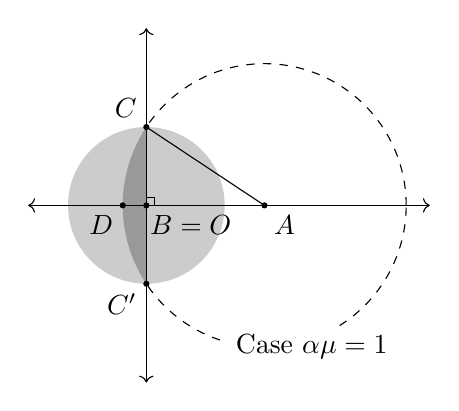
\begin{tikzpicture}[scale=1.5]
\def\m{1};
\def\L{1.2};
\fill[fill=lightgrey] (0,0) circle ({sqrt(1-2*\m+\L^2)});

\begin{scope}
\clip ({1-\m},-1.5) rectangle (-1.,1.5);
\fill[fill=medgrey] (1,0) circle (\L);
\end{scope}
\begin{scope}
\clip ({1-\m},-1.5) rectangle (2.4,1.5);
\draw[dashed] (1,0) circle (\L);
\end{scope}
%\begin{scope}
%\clip ({1-\m},-1.5) rectangle (2.5,1.5);
%\draw [dashed] (1,0) circle (\L);
%\end{scope}
%\draw[line width=1.0pt] (0.35,0) circle (1);
%\draw [dashed] (0,0) circle (.35);
%\draw [line width=1.0pt] (-.35,-0.714143) -- (-.35,0.714143);
\draw [<->] (-1.,0) -- (2.4,0);
\draw [<->] (0,-1.5) -- (0,1.5);
%\draw [dashed] ({1-\m},{sqrt(\L^2-\m^2)}) -- (0,{sqrt(\L^2-\m^2)});
%\filldraw ({1-\m},0) circle ({0.6*1.5/1.5pt}); node [below right] {$1-\alpha \mu$};
%\filldraw ({1-\L},0) circle ({0.6*1.5/1.5pt}); node [below left] {$1-\alpha L$};
%\filldraw (0,{sqrt(\L^2-\m^2)}) circle ({0.6*1.5/1.5pt}); node [below right] {$\alpha\sqrt{L^2-\mu^2}$} ;
%\filldraw (0,{sqrt(1-2*\m+\L^2)}) circle ({0.6*1.5/1.5pt}); node [above right] {$\sqrt{1-2\alpha\mu+\alpha^2 L^2}$};
\coordinate (I1) at (1,0);
\coordinate (I2) at ({1-\m},0);
\coordinate (I3) at ({1-\m},{sqrt(\L^2-\m^2)});
\coordinate (I4) at ({1-\m},{-sqrt(\L^2-\m^2)});
\coordinate (I5) at ({1-\L},0);
\draw [] (I1)-- (I3);
\tkzMarkRightAngle[size=.066666](I1,I2,I3);
\draw (I1) node[below right] {$A$};
\draw (I3) node[above left] {$C$};
\draw (I4) node[below left] {$C'$};
\draw (I5) node[below left] {$D$};
\filldraw (I1) circle ({0.6*1.5/1.5pt});
\filldraw (I3) circle ({0.6*1.5/1.5pt});
\filldraw (I4) circle ({0.6*1.5/1.5pt});
\filldraw (I5) circle ({0.6*1.5/1.5pt});
\filldraw (0,0) circle ({0.6*1.5/1.5pt});
\draw (-0.05,0) node[below right] {$B=O$};
\draw [] (0,0)-- (I3);
\draw (1.4,-1.2) node[fill=white] {Case $\alpha\mu=1$};

%
%
%\def\w{-.72};
%
%\draw[->] (-1.5,-.6)--(\w,{-sqrt(\L^2-(\w-1)^2)});
%\draw (-1.5,-.6) node [left] {$\cG\left(I-\alpha(\cM_\mu\cap \cL_L)\right)$};
%
%\def\y{.85};
%\draw[->] (1.1,-.73)--(\y,{-sqrt(1-2*\m+\L^2-\y^2)});
%\draw (1.1,-.73) node [right] {$\cG\left(\cL\left(\sqrt{1-2\alpha\mu+\alpha^2 L^2}\right)\right)$};

\end{tikzpicture}
}
&
\raisebox{-.5\height}{
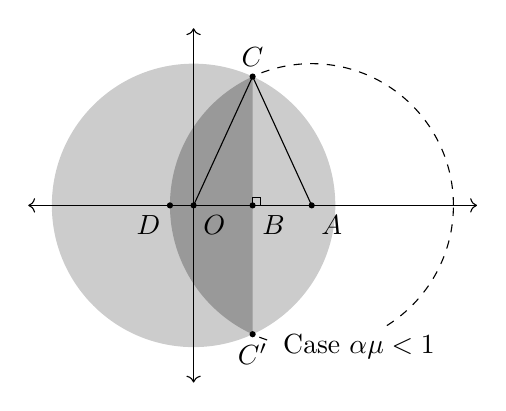
\begin{tikzpicture}[scale=1.5]
\def\m{.5};
\def\L{1.2};
\fill[fill=lightgrey] (0,0) circle ({sqrt(1-2*\m+\L^2)});

\begin{scope}
\clip ({1-\m},-1.5) rectangle (-1.4,1.5);
\fill[fill=medgrey] (1,0) circle (\L);
\end{scope}
\begin{scope}
\clip ({1-\m},-1.5) rectangle (2.4,1.5);
\draw[dashed] (1,0) circle (\L);
\end{scope}
%\begin{scope}
%\clip ({1-\m},-1.5) rectangle (2.5,1.5);
%\draw [dashed] (1,0) circle (\L);
%\end{scope}
%\draw[line width=1.0pt] (0.35,0) circle (1);
%\draw [dashed] (0,0) circle (.35);
%\draw [line width=1.0pt] (-.35,-0.714143) -- (-.35,0.714143);
\draw [<->] (-1.4,0) -- (2.4,0);
\draw [<->] (0,-1.5) -- (0,1.5);
%\draw [dashed] ({1-\m},{sqrt(\L^2-\m^2)}) -- (0,{sqrt(\L^2-\m^2)});
%\filldraw ({1-\m},0) circle ({0.6*1.5/1.5pt}); node [below right] {$1-\alpha \mu$};
%\filldraw ({1-\L},0) circle ({0.6*1.5/1.5pt}); node [below left] {$1-\alpha L$};
%\filldraw (0,{sqrt(\L^2-\m^2)}) circle ({0.6*1.5/1.5pt}); node [below right] {$\alpha\sqrt{L^2-\mu^2}$} ;
%\filldraw (0,{sqrt(1-2*\m+\L^2)}) circle ({0.6*1.5/1.5pt}); node [above right] {$\sqrt{1-2\alpha\mu+\alpha^2 L^2}$};
\coordinate (I1) at (1,0);
\coordinate (I2) at ({1-\m},0);
\coordinate (I3) at ({1-\m},{sqrt(\L^2-\m^2)});
\coordinate (I4) at ({1-\m},{-sqrt(\L^2-\m^2)});
\coordinate (I5) at ({1-\L},0);
\draw [] (I1)-- (I3);
\tkzMarkRightAngle[size=.066666](I1,I2,I3);
\draw (I1) node[below right] {$A$};
\draw (I2) node[below right] {$B$};
\draw (I3) node[above] {$C$};
\draw (I4) node[below] {$C'$};
\draw (I5) node[below left] {$D$};
\filldraw (I1) circle ({0.6*1.5/1.5pt});
\filldraw (I2) circle ({0.6*1.5/1.5pt});
\filldraw (I3) circle ({0.6*1.5/1.5pt});
\filldraw (I4) circle ({0.6*1.5/1.5pt});
\filldraw (I5) circle ({0.6*1.5/1.5pt});
\filldraw (0,0) circle ({0.6*1.5/1.5pt});
\draw (0,0) node[below right] {$O$};
\draw [] (0,0)-- (I3);
\draw (1.4,-1.2) node[fill=white] {Case $\alpha\mu<1$};

%
%
%\def\w{-.72};
%
%\draw[->] (-1.5,-.6)--(\w,{-sqrt(\L^2-(\w-1)^2)});
%\draw (-1.5,-.6) node [left] {$\cG\left(I-\alpha(\cM_\mu\cap \cL_L)\right)$};
%
%\def\y{.85};
%\draw[->] (1.1,-.73)--(\y,{-sqrt(1-2*\m+\L^2-\y^2)});
%\draw (1.1,-.73) node [right] {$\cG\left(\cL\left(\sqrt{1-2\alpha\mu+\alpha^2 L^2}\right)\right)$};

\end{tikzpicture}
}
\end{tabular}
\end{center}


The containment holds for $R$ and fails for smaller $R$.
Since $\cL_R$ is SRG-full by Theorem~\ref{thm:srg-full}, the containment of the SRG in $\ecomplex$ equivalent to the containment of the class.
% Since $\cL\left(\sqrt{1-2\alpha\mu+\alpha^2 L^2}\right)$ is SRG-representable, the inclusion of the SRG in $\ecomplex$ implies the inclusion of the class by Theorem~\ref{thm:srg-representation}.
\qed
\end{frame}

\begin{frame}
\frametitle{Convergence analysis: Forward step method}


If $\opA$ is $\mu$-strongly monotone and $\beta$-cocoercive with $0<\mu<1/\beta<\infty$,
\[
\|x^k-x^\star\|\le
\left(1-2\alpha\mu+\alpha^2\mu/\beta\right)^{k/2}
\|x^0-x^\star\|
\]
for $\alpha\in (0,2\beta)$ by Proposition~\ref{prop:sm-coco-forward}.

\vspace{0.2in}


\begin{proposition}
\label{prop:sm-coco-forward}
Let $0<\mu<1/\beta<\infty$ and $\alpha\in (0,2\beta)$.
If $\cA=\mathcal{M}_\mu\cap \mathcal{C}_\beta$, then $\opI-\alpha \cA\subseteq \cL_R$ for
\[
R= \sqrt{1-2\alpha\mu+\alpha^2\mu/\beta}.
\]
Result is tight in the sense that $\opI-\alpha\cA\nsubseteq \cL_R$ for any smaller value of $R$.
% If $A\in \mathcal{M}_\mu\cap \mathcal{C}_\beta$ and if $0<\alpha\le 2\beta$, then $I-\alpha A\in \cL\left(\sqrt{1-2\alpha\mu+\alpha^2\mu/\beta}\right)$.
\end{proposition}
\end{frame}



\begin{frame}
\frametitle{Proof of Proposition~\ref{prop:sm-coco-forward}}
\textbf{Proof.}
First consider the case  $\mu<1/(2\beta)$.
By Theorems~\ref{thm:monotone-srg} and \ref{thm:srg-scaling-translation},
\begin{center}
\begin{tabular}{cc}
\raisebox{-.5\height}{
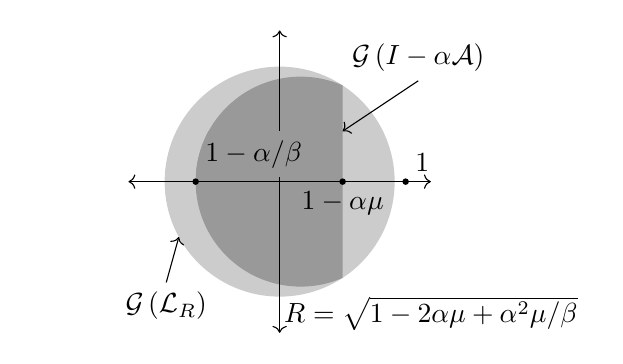
\begin{tikzpicture}[scale=1.6]
\clip (-2.,-1.222) rectangle (2.5,1.222);
\def\m{.5};
\def\b{0.6};
\fill [fill=lightgrey] (0,0) circle ({sqrt(1-2*\m+\m/\b)});
\begin{scope}
\clip ({1-\m},-1.1) rectangle (-1.1,1.1);
\fill[fill=medgrey] ({1-1/2/\b},0) circle ({1/2/\b});
\end{scope}
%\draw [dashed] (0,0) circle ({sqrt(1-2*\m+\L^2)});
\draw [<->] (-1.2,0) -- (1.2,0);
\draw [<->] (0,-1.2) -- (0,1.2);
%\draw [dashed] ({1-\m},{sqrt(\L^2-\m^2)}) -- (0,{sqrt(\L^2-\m^2)});

%\filldraw ({1-\m},{sqrt(1/4/\b^2-(\m-1/2/\b)^2)}) circle ({0.6*1.5/1.5pt});


%Draw braced note
%\draw [decorate,decoration={brace,amplitude=4.5pt}] ({sqrt(1-2*\m+\m/\b)*cos(240)},{sqrt(1-2*\m+\m/\b)*sin(240)}) -- (0,0);
%\draw [line width=1.0pt]({sqrt(1-2*\m+\m/\b)*cos(240)},{sqrt(1-2*\m+\m/\b)*sin(240)}) -- (0,0);
%\draw[->] (-1.1,-.77)--({sqrt(1-2*\m+\m/\b)*cos(240)/2-0.07},{sqrt(1-2*\m+\m/\b)*sin(240)/2+.03});
%\draw (-1.1,-.77) node[below] {$\sqrt{1-2\alpha\mu+\alpha^2\mu/\beta}$};


\coordinate (I1) at  ({1-1/\b/2},0) ;
\coordinate (I2) at ({1-\m},0);
\coordinate (I3) at ({1-\m},{sqrt(1/4/\b^2-(\m-1/2/\b)^2)});
%\draw [] (I1)-- (I3);


\filldraw (I2) circle ({0.6*1.5/1.5pt});

%\draw  ({1-1/\b/2},0.05) node [above left, fill=medgrey] {$1-1/(2\beta)$};
\filldraw ({1-\m},0) node [below ] {$1-\alpha \mu$};


\filldraw ({1-1/\b},0) circle ({0.6*1.5/1.5pt}) ;
\begin{scope}
\clip ({1-\m},-1.1) rectangle (-1.1,1.1);
\clip ({1-1/2/\b},0) circle ({1/2/\b});
\draw ({1-1/\b},0.03) node [above right, fill=medgrey] {$1-\alpha/\beta$};
\end{scope}
\filldraw (1,0) circle ({0.6*1.5/1.5pt})  node [above right] {$1$};
%\filldraw (0,{sqrt(\L^2-\m^2)}) circle ({0.6*1.5/1.5pt}) node [below right] {$\alpha\sqrt{L^2-\mu^2}$} ;
%\filldraw (0,{sqrt(1-2*\m+\L^2)}) circle ({0.6*1.5/1.5pt}) node [above right] {$\sqrt{1-2\alpha\mu+\alpha^2 L^2}$};


\coordinate (O1) at ({1-1/\b},0);
\coordinate (O2) at ({1-1/\b/2},0);
\coordinate (O3) at ({1-\m},{sqrt(1/4/\b^2-(\m-1/2/\b)^2)});


\draw[->] (1.1,.8)--({1-\m,0.4});
\draw(1.1,.8) node[above] {$\cG\left(\opI-\alpha\cA \right)$};

\def\x{-.8};
\draw[->] (-.9,-.8)--(\x,{-sqrt(1-2*\m+\m/\b-(\x)^2)});
\draw(-.9,-.8) node[below ] {$\cG\left(\cL_R\right)$};
\draw(1.2,-1.05) node[] {$R=\sqrt{1-2\alpha\mu+\alpha^2\mu/\beta}$};
\end{tikzpicture}
}
&
\!\!\!\!\!\!\!\!\!\!\!\!\!\!\!\!\!\!\!\!\!\!\!\!\!\!\!
\raisebox{-.5\height}{
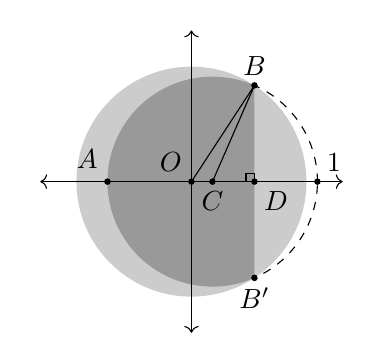
\begin{tikzpicture}[scale=1.6]
\clip (-1.3,-1.222) rectangle (1.3,1.222);
\def\m{.5};
\def\b{0.6};
\fill [fill=lightgrey] (0,0) circle ({sqrt(1-2*\m+\m/\b)});

\begin{scope}
\clip ({1-\m},-1.1) rectangle (-1.1,1.1);
\fill[fill=medgrey] ({1-1/2/\b},0) circle ({1/2/\b});
\end{scope}


\begin{scope}
\clip ({1-\m},-1.1) rectangle (1.1,1.1);
\draw[dashed] ({1-1/2/\b},0) circle ({1/2/\b});
\end{scope}


%\draw [dashed] (0,0) circle ({sqrt(1-2*\m+\L^2)});
\draw [<->] (-1.2,0) -- (1.2,0);
\draw [<->] (0,-1.2) -- (0,1.2);
%\draw [dashed] ({1-\m},{sqrt(\L^2-\m^2)}) -- (0,{sqrt(\L^2-\m^2)});

%\filldraw ({1-\m},{sqrt(1/4/\b^2-(\m-1/2/\b)^2)}) circle ({0.6*1.5/1.5pt});

%\draw [dashed] (0,0) circle ({sqrt(1-2*\m+\m/\b)});

%\draw [decorate,decoration={brace,amplitude=4.5pt}] ({sqrt(1-2*\m+\m/\b)*cos(240)},{sqrt(1-2*\m+\m/\b)*sin(240)}) -- (0,0);
%\draw [line width=1.0pt]({sqrt(1-2*\m+\m/\b)*cos(240)},{sqrt(1-2*\m+\m/\b)*sin(240)}) -- (0,0);
%\draw[->] (-1.1,-.77)--({sqrt(1-2*\m+\m/\b)*cos(240)/2-0.07},{sqrt(1-2*\m+\m/\b)*sin(240)/2+.03});
%\draw (-1.1,-.77) node[below] {$\sqrt{1-2\alpha\mu+\alpha^2\mu/\beta}$};


\coordinate (I1) at  ({1-1/\b/2},0) ;
\coordinate (I2) at ({1-\m},0);
\coordinate (I3) at ({1-\m},{sqrt(1/4/\b^2-(\m-1/2/\b)^2)});
\coordinate (I4) at ({1-\m},{-sqrt(1/4/\b^2-(\m-1/2/\b)^2)});
%\draw [] (I1)-- (I3);

\filldraw (I1) circle ({0.6*1.5/1.5pt});
\filldraw (I2) circle ({0.6*1.5/1.5pt});
\filldraw (I3) circle ({0.6*1.5/1.5pt});
\filldraw (I4) circle ({0.6*1.5/1.5pt});
\draw (I3) -- (I1);
\tkzMarkRightAngle[size=.06666](I1,I2,I3);

\draw (I1) node[below] {$C$};
\draw (I3) node[above] {$B$};
\draw (I4) node[below] {$B'$};
\draw (0,0) -- (I3);


%\draw  ({1-1/\b/2},0.05) node [above left, fill=medgrey] {$1-1/(2\beta)$};
\filldraw ({1-\m},0) node [below right ] {$D$};


\filldraw ({1-1/\b},0) circle ({0.6*1.5/1.5pt}) ;
\draw ({1-1/\b},0.03) node [above left,] {$A$};
\filldraw (1,0) circle ({0.6*1.5/1.5pt})  node [above right] {$1$};
%\filldraw (0,{sqrt(\L^2-\m^2)}) circle ({0.6*1.5/1.5pt}) node [below right] {$\alpha\sqrt{L^2-\mu^2}$} ;
%\filldraw (0,{sqrt(1-2*\m+\L^2)}) circle ({0.6*1.5/1.5pt}) node [above right] {$\sqrt{1-2\alpha\mu+\alpha^2 L^2}$};

\filldraw (0,0) circle ({0.6*1.5/1.5pt}) ;

\draw (0,0) node[above left] {$O$};
%\filldraw (I3) -- (0,0);

\coordinate (O1) at ({1-1/\b},0);
\coordinate (O2) at ({1-1/\b/2},0);
\coordinate (O3) at ({1-\m},{sqrt(1/4/\b^2-(\m-1/2/\b)^2)});


% \tkzMarkSegment[pos=.5,mark=||](O1,O2) ;
% \tkzMarkSegment[pos=.5,mark=||](O2,O3) ;
\end{tikzpicture}
}
\end{tabular}
\end{center}
To clarify, $O$ is the center of the circle with radius $\overline{OB}$ (lighter shade)
and $C$ is the center of the circle with radius $\overline{AC}=\overline{CB}$ defining the inner region (darker shade).
%The inner region (darker shade) is contained within the disk with radius  $\sqrt{1-2\alpha\mu+\alpha^2\mu/\beta}$ centered at the origin (lighter shade) by the following geometric reasoning.
\end{frame}






\begin{frame}
\frametitle{Proof of Proposition~\ref{prop:sm-coco-forward}}
With two applications of the Pythagorean theorem, we get
\begin{align*}
\overline{OB}^2
&=\overline{OD}^2+\overline{DB}^2
=\overline{OD}^2+\overline{BC}^2-\overline{CD}^2\\
&=(1-\alpha \mu)^2+(\alpha/(2\beta))^2-(\alpha/(2\beta)-\alpha \mu)^2
=1-2\alpha\mu+\alpha^2\mu/\beta.
\end{align*}
%Since $\overline{BD}^2=\overline{BC}^2-\overline{CD}^2$
Since $\overline{B'B}$ is a chord of circle $O$, it is within the circle.
Since $2$ non-identical circles intersect at at most $2$ points, and since $A$ is within circle $O$, arc $\arc{BAB'}$ is within circle $O$.
Finally, the region bounded by $\overline{B'B}\cup\arc{BAB'}$ (darker shade) is within circle $O$ (lighter shade).
\end{frame}



\begin{frame}
\frametitle{Proof of Proposition~\ref{prop:sm-coco-forward}}
When $\mu=1/(2\beta)$ and $\mu>1/(2\beta)$, geometries are slightly different but same arguments hold:
\begin{center}
\begin{tabular}{cc}
\raisebox{-.5\height}{
\!\!\!\!\!\!\!\!\!\!\!\!\!\!\!
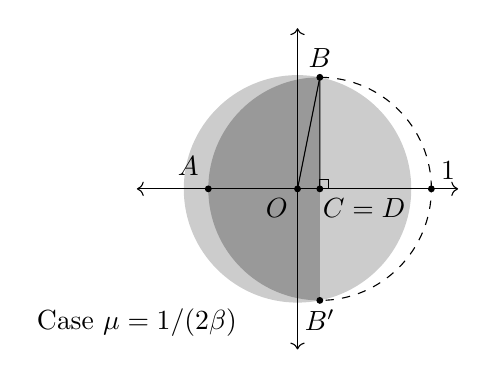
\begin{tikzpicture}[scale=1.7]
\def\m{0.8333333};
\def\b{0.6};
\fill [fill=lightgrey] (0,0) circle ({sqrt(1-2*\m+\m/\b)});

\begin{scope}
\clip ({1-\m},-1.1) rectangle (-1.1,1.1);
\fill[fill=medgrey] ({1-1/2/\b},0) circle ({1/2/\b});
\end{scope}


\begin{scope}
\clip ({1-\m},-1.1) rectangle (1.1,1.1);
\draw[dashed] ({1-1/2/\b},0) circle ({1/2/\b});
\end{scope}


%\draw [dashed] (0,0) circle ({sqrt(1-2*\m+\L^2)});
\draw [<->] (-1.2,0) -- (1.2,0);
\draw [<->] (0,-1.2) -- (0,1.2);
%\draw [dashed] ({1-\m},{sqrt(\L^2-\m^2)}) -- (0,{sqrt(\L^2-\m^2)});

%\filldraw ({1-\m},{sqrt(1/4/\b^2-(\m-1/2/\b)^2)}) circle ({0.6*1.5/1.5pt});

%\draw [dashed] (0,0) circle ({sqrt(1-2*\m+\m/\b)});

%\draw [decorate,decoration={brace,amplitude=4.5pt}] ({sqrt(1-2*\m+\m/\b)*cos(240)},{sqrt(1-2*\m+\m/\b)*sin(240)}) -- (0,0);
%\draw [line width=1.0pt]({sqrt(1-2*\m+\m/\b)*cos(240)},{sqrt(1-2*\m+\m/\b)*sin(240)}) -- (0,0);
%\draw[->] (-1.1,-.77)--({sqrt(1-2*\m+\m/\b)*cos(240)/2-0.07},{sqrt(1-2*\m+\m/\b)*sin(240)/2+.03});
%\draw (-1.1,-.77) node[below] {$\sqrt{1-2\alpha\mu+\alpha^2\mu/\beta}$};


\coordinate (I1) at  ({1-1/\b/2},0) ;
\coordinate (I2) at ({1-\m},0);
\coordinate (I3) at ({1-\m},{sqrt(1/4/\b^2-(\m-1/2/\b)^2)});
\coordinate (I4) at ({1-\m},{-sqrt(1/4/\b^2-(\m-1/2/\b)^2)});
%\draw [] (I1)-- (I3);

\filldraw (I1) circle ({0.6*1.5/1.5pt});
\filldraw (I3) circle ({0.6*1.5/1.5pt});
\filldraw (I4) circle ({0.6*1.5/1.5pt});
\draw (I3) -- (I1);
\tkzMarkRightAngle[size=.066666666666](I1,I2,I3);

\draw ({1-1/\b/2-0.05},0) node[below right] {$C=D$};
\draw (I3) node[above] {$B$};
\draw (I4) node[below] {$B'$};
\draw (0,0) -- (I3);


%\draw  ({1-1/\b/2},0.05) node [above left, fill=medgrey] {$1-1/(2\beta)$};


\filldraw ({1-1/\b},0) circle ({0.6*1.5/1.5pt}) ;
\draw ({1-1/\b},0.03) node [above left,] {$A$};
\filldraw (1,0) circle ({0.6*1.5/1.5pt})  node [above right] {$1$};
%\filldraw (0,{sqrt(\L^2-\m^2)}) circle ({0.6*1.5/1.5pt}) node [below right] {$\alpha\sqrt{L^2-\mu^2}$} ;
%\filldraw (0,{sqrt(1-2*\m+\L^2)}) circle ({0.6*1.5/1.5pt}) node [above right] {$\sqrt{1-2\alpha\mu+\alpha^2 L^2}$};

\filldraw (0,0) circle ({0.6*1.5/1.5pt}) ;

\draw (0,0) node[below left] {$O$};
%\filldraw (I3) -- (0,0);

\coordinate (O1) at ({1-1/\b},0);
\coordinate (O2) at ({1-1/\b/2},0);
\coordinate (O3) at ({1-\m},{sqrt(1/4/\b^2-(\m-1/2/\b)^2)});

\draw (-1.2,-1) node {Case $\mu=1/(2\beta)$};

% \tkzMarkSegment[pos=.5,mark=||](O1,O2) ;
% \tkzMarkSegment[pos=.5,mark=||](O2,O3) ;
\end{tikzpicture}
}
&
\raisebox{-.5\height}{
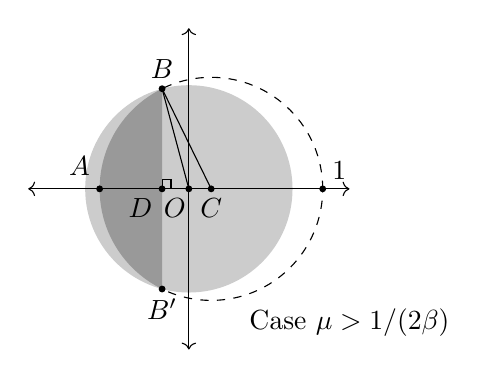
\begin{tikzpicture}[scale=1.7]
\def\m{1.2};
\def\b{0.6};
\fill [fill=lightgrey] (0,0) circle ({sqrt(1-2*\m+\m/\b)});

\begin{scope}
\clip ({1-\m},-1.1) rectangle (-1.1,1.1);
\fill[fill=medgrey] ({1-1/2/\b},0) circle ({1/2/\b});
\end{scope}


\begin{scope}
\clip ({1-\m},-1.1) rectangle (1.1,1.1);
\draw[dashed] ({1-1/2/\b},0) circle ({1/2/\b});
\end{scope}


%\draw [dashed] (0,0) circle ({sqrt(1-2*\m+\L^2)});
\draw [<->] (-1.2,0) -- (1.2,0);
\draw [<->] (0,-1.2) -- (0,1.2);
%\draw [dashed] ({1-\m},{sqrt(\L^2-\m^2)}) -- (0,{sqrt(\L^2-\m^2)});

%\filldraw ({1-\m},{sqrt(1/4/\b^2-(\m-1/2/\b)^2)}) circle ({0.6*1.5/1.5pt});

%\draw [dashed] (0,0) circle ({sqrt(1-2*\m+\m/\b)});

%\draw [decorate,decoration={brace,amplitude=4.5pt}] ({sqrt(1-2*\m+\m/\b)*cos(240)},{sqrt(1-2*\m+\m/\b)*sin(240)}) -- (0,0);
%\draw [line width=1.0pt]({sqrt(1-2*\m+\m/\b)*cos(240)},{sqrt(1-2*\m+\m/\b)*sin(240)}) -- (0,0);
%\draw[->] (-1.1,-.77)--({sqrt(1-2*\m+\m/\b)*cos(240)/2-0.07},{sqrt(1-2*\m+\m/\b)*sin(240)/2+.03});
%\draw (-1.1,-.77) node[below] {$\sqrt{1-2\alpha\mu+\alpha^2\mu/\beta}$};


\coordinate (I1) at  ({1-1/\b/2},0) ;
\coordinate (I2) at ({1-\m},0);
\coordinate (I3) at ({1-\m},{sqrt(1/4/\b^2-(\m-1/2/\b)^2)});
\coordinate (I4) at ({1-\m},{-sqrt(1/4/\b^2-(\m-1/2/\b)^2)});
%\draw [] (I1)-- (I3);

\filldraw (I1) circle ({0.6*1.5/1.5pt});
\filldraw (I2) circle ({0.6*1.5/1.5pt});
\filldraw (I3) circle ({0.6*1.5/1.5pt});
\filldraw (I4) circle ({0.6*1.5/1.5pt});
\draw (I3) -- (I1);
\tkzMarkRightAngle[size=.06666666666](I1,I2,I3);

\draw (I1) node[below] {$C$};
\draw (I3) node[above] {$B$};
\draw (I4) node[below] {$B'$};
\draw (0,0) -- (I3);


%\draw  ({1-1/\b/2},0.05) node [above left, fill=medgrey] {$1-1/(2\beta)$};
\filldraw ({1-\m},0) node [below left ] {$D$};


\filldraw ({1-1/\b},0) circle ({0.6*1.5/1.5pt}) ;
\draw ({1-1/\b},0.03) node [above left,] {$A$};
\filldraw (1,0) circle ({0.6*1.5/1.5pt})  node [above right] {$1$};
%\filldraw (0,{sqrt(\L^2-\m^2)}) circle ({0.6*1.5/1.5pt}) node [below right] {$\alpha\sqrt{L^2-\mu^2}$} ;
%\filldraw (0,{sqrt(1-2*\m+\L^2)}) circle ({0.6*1.5/1.5pt}) node [above right] {$\sqrt{1-2\alpha\mu+\alpha^2 L^2}$};

\filldraw (0,0) circle ({0.6*1.5/1.5pt}) ;

\draw (0.05,0) node[below left] {$O$};
%\filldraw (I3) -- (0,0);

\coordinate (O1) at ({1-1/\b},0);
\coordinate (O2) at ({1-1/\b/2},0);
\coordinate (O3) at ({1-\m},{sqrt(1/4/\b^2-(\m-1/2/\b)^2)});

\draw (1.2,-1) node {Case $\mu>1/(2\beta)$};


% \tkzMarkSegment[pos=.5,mark=||](O1,O2) ;
% \tkzMarkSegment[pos=.5,mark=||](O2,O3) ;
\end{tikzpicture}
}
\end{tabular}
\end{center}

The containment holds for $R$ and fails for smaller $R$.
Since $\cL_R$ is SRG-full by Theorem~\ref{thm:srg-full}, the containment of the SRG in $\ecomplex$ equivalent to the containment of the class.
% Since $\cL\left(\sqrt{1-2\alpha\mu+\alpha^2\mu/\beta}\right)$ is SRG-representable, the inclusion of the SRG in $\ecomplex$ implies the inclusion of the class by Theorem~\ref{thm:srg-representation}.
\qed
\end{frame}


\begin{frame}
\frametitle{Inversive geometry}
 Generalized circles consist of (finite) circles and lines with $\{\infty\}$. \\
 (A line is like a circle with infinite radius.)
 
 \vspace{0.2in}
 Inversion maps generalized circles to generalized circles.
 
 \vspace{0.2in}

In complex analysis, the inversion map is known as the M\"obius transformation.
 In classical Euclidean geometry, inversive geometry considers generally the inversion of the 2D plane about any circle but our inversion map $z\mapsto\bar{z}^{-1}$ is the inversion about the unit circle.

\end{frame}


\begin{frame}[plain]
\frametitle{Inverting generalized circles}
\begin{center}
\begin{tabular}{cccc}
\raisebox{-.5\height}{
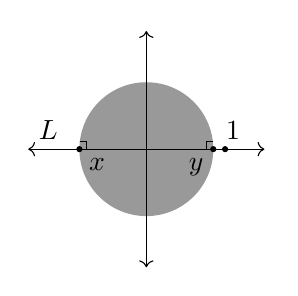
\begin{tikzpicture}[scale=1.0]
%\draw[dashed] (0,0) circle (1);
\def\r{0.85}
\fill[fill=medgrey] (0,0) circle (\r);
\draw [<->] (-1.5,0) -- (1.5,0);
\draw (-1,0) node [above left] {$L$};
\draw [<->] (0,-1.5) -- (0,1.5);
\draw (\r,0) node [below left] {$y$};
\filldraw (\r,0) circle  ({0.6*1.5/1.0pt});
\draw (-\r,0) node [below right] {$x$};
\filldraw (-\r,0) circle  ({0.6*1.5/1.0pt});
\filldraw (1,0) circle  ({0.6*1.5/1.0pt});
\draw (1.1,0) node [above] {$1$};
%\draw (0,-1.7) node {$C(e_1,a,b)$};
\draw (.95,1.25) node {\phantom{$\cup \{\binfty\}$}};

\begin{scope}
\clip (0,0) circle (\r);
\coordinate (A) at (-0.4,0) {};
\coordinate (B) at ({-\r-0.01},0) {};
\coordinate (C) at ({-\r-0.01},1) {};
\tkzMarkRightAngle[size=.1](A,B,C);
\end{scope}

\begin{scope}
\clip (0,0) circle (\r);
\coordinate (A) at (0.4,0) {};
\coordinate (B) at ({\r+0.01},0) {};
\coordinate (C) at ({\r+0.01},1) {};
\tkzMarkRightAngle[size=.1](A,B,C);
\end{scope}

\end{tikzpicture}}
&
\raisebox{-.5\height}{
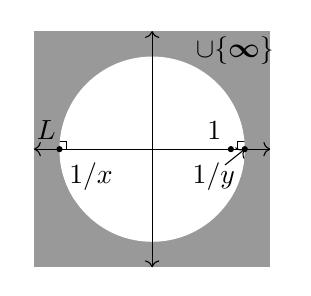
\begin{tikzpicture}[scale=1.0]

\def\r{0.85}
\fill[fill=medgrey] (-1.5,-1.5) rectangle (1.5,1.5);
\fill[fill=white] (0,0) circle (1/\r);
\draw [<->] (-1.5,0) -- (1.5,0);
\draw (-1.1,0) node [above left] {$L$};
\draw [<->] (0,-1.5) -- (0,1.5);
\filldraw (1,0) circle  ({0.6*1.5/1.0pt});
\draw (1,0) node [above left] {$1$};
\begin{scope}
\clip (0,0) circle (1/\r);
%\draw[dashed] (0,0) circle (1);
\draw ({1/\r-0.0},-0.05) node [below left, fill=white] {$1/y$};
\draw ({-1/\r-0.0},-0.05) node [below right, fill=white] {$1/x$};
\end{scope}
\filldraw ({1/\r},0) circle ({0.6*1.5/1.0pt});
\draw [->] ({1/\r-0.25},-0.2) -- ({1/\r},0);
\filldraw ({-1/\r},0) circle ({0.6*1.5/1.0pt});
\draw (1.05,1.25) node {$\cup \{\binfty\}$};
%\draw (0,-1.7) node {$C(e_1,b^{-1},a^{-1})$};

\begin{scope}
\clip (0,0) circle ({(1/\r)});
\coordinate (A) at (-0.4,0) {};
\coordinate (B) at ({-(1/\r)-0.01},0) {};
\coordinate (C) at ({-(1/\r)-0.01},1) {};
\tkzMarkRightAngle[size=.1](A,B,C);
\end{scope}

\begin{scope}
\clip (0,0) circle ({(1/\r)});
\coordinate (A) at (0.4,0) {};
\coordinate (B) at ({(1/\r)+0.01},0) {};
\coordinate (C) at ({(1/\r)+0.01},1) {};
\tkzMarkRightAngle[size=.1](A,B,C);
\end{scope}
\end{tikzpicture}}
\end{tabular}
\end{center}

\begin{enumerate}
    \item Draw a line $L$ through the origin orthogonally intersecting the generalized circle. This means $L$ intersects the boundary perpendicularly, which implies $L$ goes through the circle's center when the generalized circle is finite.
\item Let $-\infty<x< y\le \infty$ represent the signed distance of the intersecting points from the origin along this line.
If the generalized circle is a line, then $y=\infty$.
%If $x,y$ are on the opposite side of the origin, then $x<0$.
\item Draw a generalized circle orthogonally intersecting $L$ at $(1/x)$ and $(1/y)$.
\item When inverting a region with a generalized circle as the boundary, pick a point on $L$ within the interior of the region to determine on which side of the boundary the inverted interior lies.
\end{enumerate}

\end{frame}




\begin{frame}
\frametitle{Example: Inverting generalized circles}
\begin{center}
\raisebox{-.5\height}{
\!\!\!\!\!\!\!\!\!\!\!\!
\begin{tabular}{ccc}
\raisebox{-.5\height}{
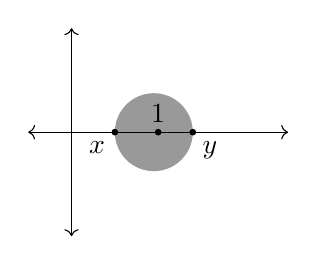
\begin{tikzpicture}[scale=1.1]
\def\a{0.5}
\def\b{1.4}
\fill[fill=medgrey] ({(\a+\b)/2},0) circle ({(\b-\a)/2});
\draw [<->] (-.5,0) -- (2.5,0);
\draw [<->] (0,-1.2) -- (0,1.2);
\filldraw (\a,0) circle  ({0.6*1.5/1.0pt});
\draw (\a,0) node [below left] {$x$};
\filldraw (\b,0) circle  ({0.6*1.5/1.0pt});
\draw (\b,0) node [below right] {$y$};
\filldraw (1,0) circle  ({0.6*1.5/1.0pt});
\draw (1,0) node [above] {$1$};
%\draw (1,-1.7) node {$C(e_1,c,d)$};
\draw ({1/\a+.23},0) node [below] {\phantom{$x^{-1}$}};
\end{tikzpicture}}
&
\raisebox{-.5\height}{
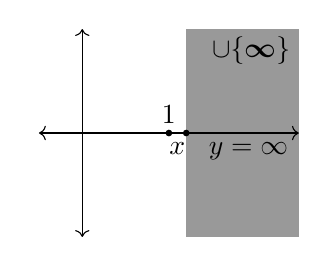
\begin{tikzpicture}[scale=1.1]
\def\m{1.2}
\fill[fill=medgrey] (\m,-1.2) rectangle (2.5,1.2);
\draw [<->] (-.5,0) -- (2.5,0);
\draw [<->] (0,-1.2) -- (0,1.2);
\filldraw ({(\m)},0) circle  ({0.6*1.5/1.0pt});
\draw ({(\m)+0.1},0) node [below left] {$x$};
\filldraw (1,0) circle  ({0.6*1.5/1.0pt});
\draw (1,0) node [above] {$1$};
\draw (1.95,0.95) node {$\cup \{\binfty\}$};
\draw (1.35,0) node [below right] {$y=\infty$};
%\draw (1,-1.7) node {$C(e_1,f,\infty)$};
\draw (0.1,0) node [below left] {\phantom{$y^{-1}$}};
\end{tikzpicture}}
&
\raisebox{-.5\height}{
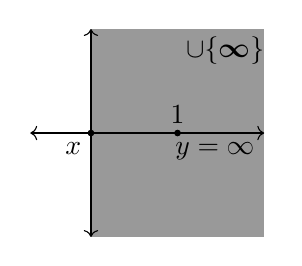
\begin{tikzpicture}[scale=1.1]
\fill[fill=medgrey] (0,-1.2) rectangle (2,1.2);
\draw [<->] (-0.7,0) -- (2,0);
\draw [<->] (0,-1.2) -- (0,1.2);
\filldraw (1,0) circle  ({0.6*1.5/1.0pt});
\draw (1,0) node [above] {$1$};
\filldraw (0,0) circle  ({0.6*1.5/1.0pt});
\draw (0,0) node [below left] {$x$};
\draw (0,0) node [below left] {\phantom{$y^{-1}$}};
\draw (1.55,.95) node {$\cup \{\binfty\}$};
\draw (2,0) node [below left] {$y=\infty$};
%\draw (0,-1.7) node {$C(e_1,0,\infty)$};
\end{tikzpicture}}
\end{tabular}}
\\
\raisebox{-.5\height}{
\!\!\!\!\!\!\!\!\!\!\!\!
\begin{tabular}{ccc}
\raisebox{-.5\height}{
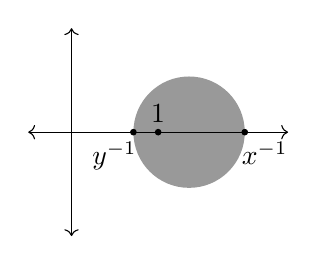
\begin{tikzpicture}[scale=1.1]
\def\a{0.5}
\def\b{1.4}
\fill[fill=medgrey] ({(1/\a+1/\b)/2},0) circle ({(1/\a-1/\b)/2});
\draw [<->] (-.5,0) -- (2.5,0);
\draw [<->] (0,-1.2) -- (0,1.2);
\filldraw ({1/\a},0) circle  ({0.6*1.5/1.0pt});
\draw ({1/\a+.23},0) node [below] {$x^{-1}$};
\filldraw ({1/\b},0) circle  ({0.6*1.5/1.0pt});
\draw ({1/\b+.15},0) node [below left] {$y^{-1}$};
\filldraw (1,0) circle  ({0.6*1.5/1.0pt});
\draw (1,0) node [above] {$1$};
%\draw (1,-1.7) node {$C(e_1,d^{-1},c^{-1})$};
\end{tikzpicture}}
&
\raisebox{-.5\height}{
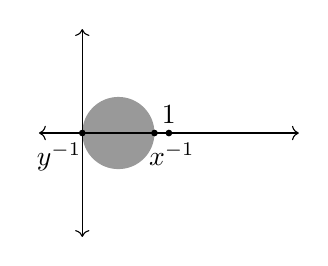
\begin{tikzpicture}[scale=1.1]
\def\m{1.2}
\fill[fill=medgrey] ({(1/\m)/2},0) circle ({(1/\m)/2});
\draw [<->] (-.5,0) -- (2.5,0);
\draw [<->] (0,-1.2) -- (0,1.2);
\filldraw (0,0) circle  ({0.6*1.5/1.0pt});
\draw (0.1,0) node [below left] {$y^{-1}$};
\filldraw ({(1/\m)},0) circle  ({0.6*1.5/1.0pt});
\draw ({(1/\m)+0.2},0) node [below ] {$x^{-1}$};
\filldraw (1,0) circle  ({0.6*1.5/1.0pt});
\draw (1,0) node [above] {$1$};
%\draw (1,-1.7) node {$C(e_1,0,f^{-1})$};
\draw (1.95,0.95) node {\phantom{$\cup \{\binfty\}$}};
\end{tikzpicture}}
&
\raisebox{-.5\height}{
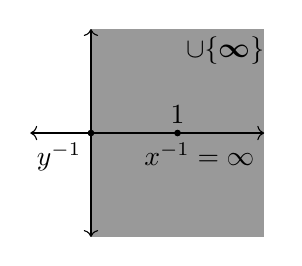
\begin{tikzpicture}[scale=1.1]
\fill[fill=medgrey] (0,-1.2) rectangle (2,1.2);
\draw [<->] (-0.7,0) -- (2,0);
\draw [<->] (0,-1.2) -- (0,1.2);
\filldraw (1,0) circle  ({0.6*1.5/1.0pt});
\filldraw (0,0) circle  ({0.6*1.5/1.0pt});
\draw (0,0) node [below left] {$y^{-1}$};
\draw (1,0) node [above] {$1$};
\draw (1.55,.95) node {$\cup \{\binfty\}$};
\draw (2,0) node [below left] {$x^{-1}=\infty$};
%\draw (0,-1.7) node {$C(e_1,0,\infty)$};
\end{tikzpicture}}
\end{tabular}}
\end{center}
\end{frame}


\begin{frame}
\frametitle{Inversion}
We relate inversion of operators with inversion (reciprocal) of complex numbers and utilize inversive geometry.


\begin{theorem}
\label{thm:srg-inversion}
If $\cA$ is a class of operators, then 
\[
\cG(\cA^{-1})=\left(\cG(\cA)\right)^{-1}.
\]
If $\cA$ is furthermore SRG-full, then $\cA^{-1}$ is  SRG-full.
\end{theorem}
% Since a class of operators can consist of a single operator,
% %Theorem~\ref{thm:srg-inversion} implies that
% if $\opA\colon\reals^n\rightrightarrows\reals^n$, then
% $\cG(\opA^{-1})=(\cG(\opA))^{-1}$.
\vspace{0.2in}


To clarify, $(\cG(\cA))^{-1}=\{z^{-1}\,|\,z\in \cG(\cA)\}\subseteq\ecomplex$.

\vspace{0.2in}
Note $(\cG(\cA))^{-1}=(\overline{\cG(\cA)})^{-1}$, since $\cG(\cA)$ is symmetric about real axis, so we write the simpler $(\cG(\cA))^{-1}$ even though inversion map is $z\mapsto \bar{z}^{-1}$.
\end{frame}




\begin{frame}[plain]
\frametitle{Convergence analysis: proximal point}
Consider
\[
\begin{array}{ll}
\underset{x\in \reals^n}{\mbox{find}}&0\in \opA x,
\end{array}
\]
where $\opA$ is maximal $\mu$-strongly monotone.
PPM
\[
x^{k+1}=\opJ_{\alpha \opA}x^k
\]
 converges exponentially with rate 
\[
\|x^k-x^\star\|\le
\left(\frac{1}{1+\alpha\mu}\right)^k
\|x^0-x^\star\|
\]
for $\alpha>0$ by the following Proposition~\ref{prop:sm-res}.
\vspace{0.2in}



\begin{proposition}
\label{prop:sm-res}
Let $\mu\in(0,\infty)$ and $\alpha\in(0,\infty)$.
If $\cA=\mathcal{M}_\mu$, then 
$\opJ_{\alpha \cA}\subseteq \cL_R$
for
\[
R= \frac{1}{1+\alpha\mu}.
\]
Result is tight in the sense that $\opJ_{\alpha \cA}\nsubseteq \cL_R$ for any smaller value of $R$.
% If $A\in \mathcal{M}_\mu$, then 
% \[
% J_{\alpha A}\in \cL\left(\frac{1}{1+\alpha\mu}\right).
% \]
\end{proposition}
\end{frame}


\begin{frame}
\textbf{Proof.}
By Theorems~\ref{thm:monotone-srg}, \ref{thm:srg-scaling-translation}, and \ref{thm:srg-inversion}, we have 
\begin{center}
\raisebox{-.5\height}{
\!\!\!\!\!\!\!\!\!\!\!\!
\begin{tabular}{ccc}
\raisebox{-.5\height}{
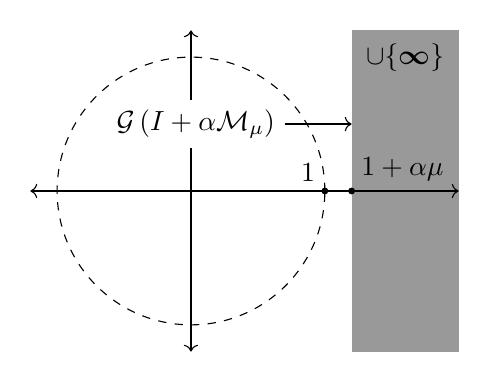
\begin{tikzpicture}[scale=1.7]
\clip (-1.22,-1.22) rectangle (2.02,1.22);
\fill[fill=medgrey] (1.2,-1.2) rectangle (2,1.2);
\draw (1.2,0.) node [above right] {$1+\alpha\mu$};
\draw (1.6,1) node {$\cup \{\binfty\}$};
\draw [<->] (-1.2,0) -- (2,0);
\draw [<->] (0,-1.2) -- (0,1.2);
\draw [dashed] (0,0) circle (1);
\draw (1,-0) node [above left] {$1$};
\filldraw (1,0) circle ({0.6*1.5/1.5pt});
\filldraw (1.2,0)  circle ({0.6*1.5/1.5pt});
\draw [->] (0.7,.5) -- (1.2,0.5);
\draw (0.7,.5) node [left, fill=white] {$\cG\left(\opI+\alpha \cM_\mu\right)$};
\end{tikzpicture}}
&
\!\!\!
$\stackrel{\bar{z}^{-1}}{\longrightarrow}$
\!\!\!\!\!\!\!\!
&
\raisebox{-.5\height}{
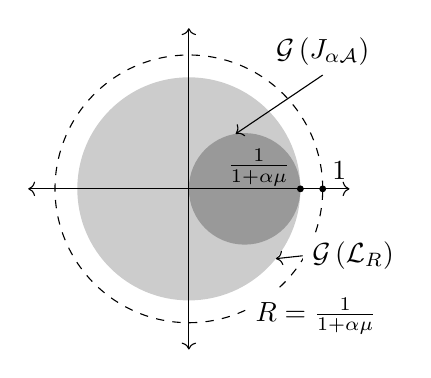
\begin{tikzpicture}[scale=1.7]
%\clip (-1.22,-1.22) rectangle (1.5,1.22);
\fill [fill=lightgrey] (0,0) circle (0.83333333333);
\fill[fill=medgrey] (0.41666666666,0) circle (0.41666666666);
\draw [<->] (-1.2,0) -- (1.2,0);
\draw [<->] (0,-1.2) -- (0,1.2);
\draw [dashed] (0,0) circle (1);
\draw (1,-0pt) node [above right] {$1$};
\filldraw (1,0) circle ({0.6*1.5/1.5pt});
\filldraw ((0.83333333333,0)  circle ({0.6*1.5/1.5pt});
\draw (0.83,-.05) node [above left] {$\frac{1}{1+\alpha\mu}$};
\def\x{0.35}
\draw [->] (1.,.85) -- (\x,{sqrt((0.833333/2)^2-(\x-(0.833333/2))^2)});
\draw (1.,.85) node [above] {$\cG\left(\opJ_{\alpha \cA}\right)$};
%\draw (-1.2,1.) node [above, fill=white] {$\cG\left(\left(I+\alpha \cM_\mu\right)^{-1}\right)$};


\def\y{0.65}
\draw [->] (.85,-.5) -- (\y,{-sqrt((0.833333)^2-(\y)^2)});
\draw (.85,-.5) node [right, fill=white] {$\cG\left(\cL_R\right)$};
\draw (.95,-.95) node [fill=white] {$R=\frac{1}{1+\alpha\mu}$};

\end{tikzpicture}}
\end{tabular}
}
\end{center}

The containment holds for $R$ and fails for smaller $R$.
Since $\cL_R$ is SRG-full by Theorem~\ref{thm:srg-full}, the containment of the SRG in $\ecomplex$ equivalent to the containment of the class.\qed
\end{frame}


\begin{frame}[plain]
\frametitle{Convergence analysis: DRS}
Consider 
\[
\begin{array}{ll}
\underset{x\in \reals^n}{\mbox{find}}&0\in (\opA+\opB) x,
\end{array}
\]
where $\opA\in \cM_\mu\cap \cC_\beta$ and $\opB\in\cM$ are maximal monotone.
DRS
\[
z^{k+1}=\left(\tfrac{1}{2}\opI+\tfrac{1}{2}\opR_{\alpha \opA}\opR_{\alpha \opB}\right)z^k
\]
converges exponentially with rate 
\[
\|z^k-z^\star\|\le
\left(
\frac{1}{2}+\frac{1}{2}
\sqrt{1-\frac{4\alpha\mu}{1+2\alpha\mu+\alpha^2\mu/\beta}}\right)^k
\|z^0-z^\star\|
\]
for $\alpha>0$ by the following Proposition~\ref{prop:refl-sm-coco} and Exercise~13.9.


\vspace{0.2in}


\begin{proposition}
\label{prop:refl-sm-coco}
Let $0<\mu<1/\beta<\infty$ and $\alpha\in(0,\infty)$.
If $\cA= \cM_\mu\cap \cC_\beta$, then $\opR_{\alpha \cA}\subseteq \cL_R$ for
\[
R=\sqrt{1-\frac{4\alpha\mu}{1+2\alpha\mu+\alpha^2\mu/\beta}}.
\]
Result is tight in the sense that $\opR_{\alpha \cA}\nsubseteq \cL_R$ for any smaller value of $R$.
\end{proposition}
\end{frame}


\begin{frame}
\textbf{Proof.}
By Theorems~\ref{thm:monotone-srg}, \ref{thm:srg-scaling-translation}, and \ref{thm:srg-inversion}, 
\vspace{-0.15in}
\begin{center}
\begin{tabular}{ccccc}
\raisebox{-.5\height}{
\!\!\!\!\!\!\!\!\!\!\!\!\!\!\!\!
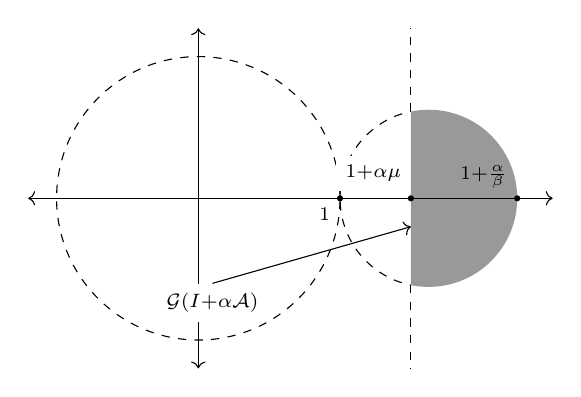
\begin{tikzpicture}[scale=1.8]
\def\m{0.5};
\def\b{.8};
\begin{scope}
\clip ({1+\m},-1.2) rectangle (-1.2,1.2);
\draw[dashed] ({1+1/2/\b},0) circle ({1/2/\b});
\end{scope}
\draw [dashed] ({1+\m},{sqrt((1/2/\b)^2-(1/2/\b-\m)^2)}) -- ({1+\m},1.2);
\draw [dashed] ({1+\m},{-sqrt((1/2/\b)^2-(1/2/\b-\m)^2)}) -- ({1+\m},-1.2);

\begin{scope}
\clip ({1+\m},-1.2) rectangle (2.5,1.2);
\fill[fill=medgrey] ({1+1/2/\b},0) circle ({1/2/\b});
%\draw[line width=1.0pt] ({1+1/2/\b},0) circle ({1/2/\b});
% \fill[fill=medgrey] (1.2,-1.2) rectangle (2,1.2);
% \draw [line width=1.0pt] (1.2,-1.2) -- (1.2,1.2);
% \fill[fill=black!60] (1.3,0) circle (0.3);
% \draw[line width=1.0pt] (1.3,0) circle (0.3);
\end{scope}
\begin{scope}
\clip ({1+1/2/\b},0) circle ({1/2/\b});
%\draw [line width=1.0pt] ({1+\m},-1.2) -- ({1+\m},1.2);
\end{scope}
\filldraw ({1+\m},0)circle ({0.6*1.5/1.8pt});
\filldraw ({1+1/\b},0)  circle ({0.6*1.5/1.8pt});


\draw ({1+1/\b},0.0) node [above left] {$\scriptstyle1+\frac{\alpha}{\beta}$};
\draw [<->] (-1.2,0) -- (2.5,0);
\draw [<->] (0,-1.2) -- (0,1.2);
\draw [dashed] (0,0) circle (1);
\draw ({1+\m},0.05) node [above left,fill=white] {$\scriptstyle 1+\alpha\mu$};
\draw (1,-0pt) node [below left] {$\scriptstyle 1$};
\filldraw (1,0)circle ({0.6*1.5/1.8pt});
%\draw (.2,-.8) node [below,fill=white] {$\cG\left(I+\alpha(\cM_\mu\cap \cC_\beta)\right)$};
\draw (.1,-.6) node [below,fill=white] {$\scriptstyle\cG\left(\opI+\alpha\cA\right)$};
\draw [->] (.1,-.6) -- ({1+\m},-0.2);
\end{tikzpicture}}
&\!\!\!\!\!\!\!
$\stackrel{\bar{z}^{-1}}{\longrightarrow}$
&\!\!\!\!\!\!\!\!\!\!
\raisebox{-.5\height}{
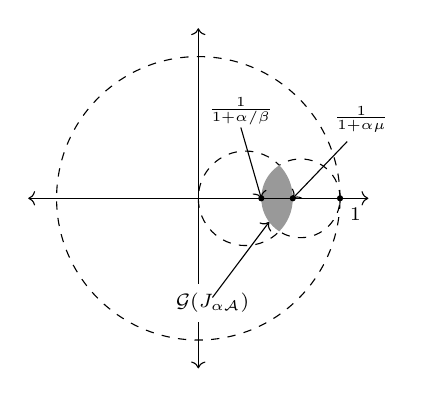
\begin{tikzpicture}[scale=1.8]
\def\m{0.5};
\def\b{.8};


\begin{scope}
\clip ({1/2*(-\m/(1+\m)+sqrt(1/(1 + \m)/(1 + \m) + (4*\b*\m*(-1 + \b*\m))/(\b + \m + 2*\b*\m)/(\b + \m + 2*\b*\m)))+1/2},-1.2)  rectangle (-1.2,1.2);
\draw[dashed] ({1/(1+\m)/2},0) circle ({1/(1+\m)/2});
\end{scope}


\begin{scope}
\clip ({1/2*(-\m/(1+\m)+sqrt(1/(1 + \m)/(1 + \m) + (4*\b*\m*(-1 + \b*\m))/(\b + \m + 2*\b*\m)/(\b + \m + 2*\b*\m)))+1/2},-1.2)  rectangle (1.2,1.2);
\draw[dashed] ({(1+2*\b)/(2+2*\b)},0) circle ({(1)/(2+2*\b)});
\end{scope}

\begin{scope}
\clip ({1/(1+\m)/2},0) circle ({1/(1+\m)/2});
\fill[fill=medgrey] ({(1+2*\b)/(2+2*\b)},0) circle ({(1)/(2+2*\b)});
%\draw[line width=1.0pt] ({(1+2*\b)/(2+2*\b)},0) circle ({(1)/(2+2*\b)});
\end{scope}
\begin{scope}
\clip ({(1+2*\b)/(2+2*\b)},0) circle ({(1)/(2+2*\b)});
%\draw[line width=1.0pt] ({1/(1+\m)/2},0) circle ({1/(1+\m)/2});
\end{scope}
\draw [<->] (-1.2,0) -- (1.2,0);
\draw [<->] (0,-1.2) -- (0,1.2);
\draw [dashed] (0,0) circle (1);
\draw (1,-0pt) node [below right] {$\scriptstyle 1$};
\filldraw (1,0)circle ({0.6*1.5/1.8pt});

\filldraw ({1/(1+\m)},0)circle ({0.6*1.5/1.8pt});
\draw[->] (1.05,.4)--({1/(1+\m)},0);
\draw (1.15,.4) node [above] {$\scriptstyle\frac{1}{1+\alpha\mu}$};

\filldraw ({1/(1+1/\b)},0)circle ({0.6*1.5/1.8pt});
\draw[->] (.3,.5)--({1/(1+1/\b)},0);
\draw (.3,.45) node [above] {$\scriptstyle\frac{1}{1+\alpha/\beta}$};


\def\x{.5}
%\draw (.1,-.7) node [below,fill=white] {$\cG\left(\left(I+\alpha(\cM_\mu\cap \cC_\beta)\right)^{-1}\right)$};
%\draw (.1,-.7) node [below,fill=white] {$\cG\left(\left(I+\alpha\cA\right)^{-1}\right)$};
\draw (.1,-.6) node [below,fill=white] {$\scriptstyle\cG\left(\opJ_{\alpha \cA}\right)$};
\draw [->] (.1,-.7) -- (\x,{-sqrt(((1)/(2+2*\b))^2-(\x-(1+2*\b)/(2+2*\b))^2)});
\end{tikzpicture}}\\
&\!\!\!\!\!\!\!\!\!\!\!\!\!\!
$\stackrel{2z-1}{\longrightarrow}$
&\!\!\!\!\!\!\!\!\!\!\!\!\!\!\!\!
\raisebox{-.5\height}{
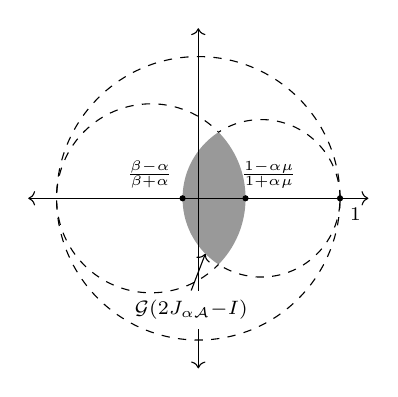
\begin{tikzpicture}[scale=1.8]
\def\m{0.5};
\def\b{.8};
%\fill [fill=lightgrey] (0,0) circle ({sqrt((\b + \m - 2*\b*\m)/   (\b + \m + 2*\b*\m))});



\begin{scope}
\clip ({-\m/(1+\m)},0) circle ({1-\m/(1+\m)});
\fill[fill=medgrey] ({1/(1+1/\b)},0) circle ({1-1/(1+1/\b)});
%\draw[line width=1.0pt] ({1/(1+1/\b)},0) circle ({1-1/(1+1/\b)});
\end{scope}

\draw [<->] (-1.2,0) -- (1.2,0);
\draw [<->] (0,-1.2) -- (0,1.2);

\def\x{.05};
\draw (-.05,-.65) node [below,fill=white] {$\scriptstyle\cG\left(2\opJ_{\alpha \cA}-\opI\right)$};
\draw [->] (-.05,-.65) -- (\x,{-sqrt(((2)/(2+2*\b))^2-(\x-2*(1+2*\b)/(2+2*\b)+1)^2)});
\begin{scope}
\clip ({-\m/(1+\m)+sqrt(1/(1 + \m)/(1 + \m) + (4*\b*\m*(-1 + \b*\m))/(\b + \m + 2*\b*\m)/(\b + \m + 2*\b*\m))},-1.2)  rectangle (-1.2,1.2);
\draw[dashed] ({-\m/(1+\m)},0) circle ({1-\m/(1+\m)});
\end{scope}

\begin{scope}
\clip ({-\m/(1+\m)+sqrt(1/(1 + \m)/(1 + \m) + (4*\b*\m*(-1 + \b*\m))/(\b + \m + 2*\b*\m)/(\b + \m + 2*\b*\m))},-1.2)  rectangle (1.2,1.2);
\draw[dashed] ({1/(1+1/\b)},0) circle ({1-1/(1+1/\b)});
\end{scope}


\begin{scope}
\clip ({1/(1+1/\b)},0) circle ({1-1/(1+1/\b)});
%\draw[line width=1.0pt] ({-\m/(1+\m)},0) circle ({1-\m/(1+\m)});
\end{scope}
\draw [dashed] (0,0) circle (1);
\draw (1,-0pt) node [below right] {$\scriptstyle1$};
\filldraw (1,0)circle ({0.6*1.5/1.8pt});
\filldraw ({(1-\m)/(1+\m)},0)circle ({0.6*1.5/1.8pt});
\draw ({(1-\m)/(1+\m)-0.1},0) node [above right] {$\scriptstyle\frac{1-\alpha\mu}{1+\alpha\mu}$};
\filldraw ({(1-1/\b)/(1+1/\b)},0)circle ({0.6*1.5/1.8pt});
\draw ({(1-1/\b)/(1+1/\b)},0) node [above left] {$\scriptstyle\frac{\beta-\alpha}{\beta+\alpha}$};

%\draw (-.1,-.9) node [below,fill=white] {$\cG\left(2\left(I+\alpha(\cM_\mu\cap \cC_\beta)\right)^{-1}-I\right)$};


%
%\def\y{.3}
%\draw [->] (.4,.7) -- (\y,{sqrt((sqrt((\b + \m - 2*\b*\m)/   (\b + \m + 2*\b*\m)))^2-(\y)^2)});
%\draw (.4,.7) node [above,fill=white] {$\cG\left(\cL\left(\sqrt{1-\frac{4\alpha\mu}{1+2\alpha\mu+\alpha^2\mu/\beta}}\right)\right)$};


\end{tikzpicture}}
\end{tabular}
\end{center}
\end{frame}

\begin{frame}
A closer look gives us
%------------------------------------------------------------------------------
\begin{center}
\raisebox{-.5\height}{
\!\!\!\!\!\!\!\!\!\!\!\!\!\!\!
\!\!\!\!\!\!\!\!\!\!\!\!\!
\begin{tabular}{cc}
\raisebox{-.5\height}{
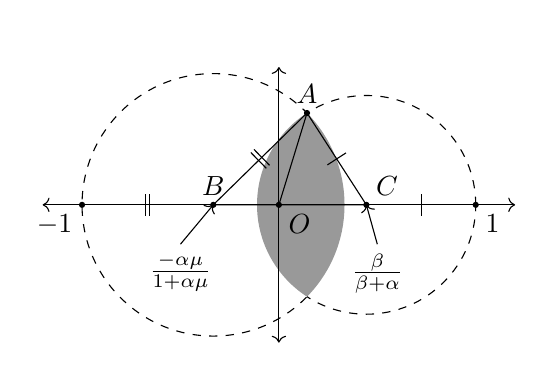
\begin{tikzpicture}[scale=2.5]
\def\m{0.5};
\def\b{.8};
\begin{scope}
\clip ({-\m/(1+\m)+sqrt(1/(1 + \m)/(1 + \m) + (4*\b*\m*(-1 + \b*\m))/(\b + \m + 2*\b*\m)/(\b + \m + 2*\b*\m))},-0.7)  rectangle (-1.2,0.9);
\draw[dashed] ({-\m/(1+\m)},0) circle ({1-\m/(1+\m)});
\end{scope}


\begin{scope}
\clip ({-\m/(1+\m)+sqrt(1/(1 + \m)/(1 + \m) + (4*\b*\m*(-1 + \b*\m))/(\b + \m + 2*\b*\m)/(\b + \m + 2*\b*\m))},-0.7)  rectangle (1.2,0.9);
\draw[dashed] ({1/(1+1/\b)},0) circle ({1-1/(1+1/\b)});
\end{scope}



\begin{scope}
\clip ({-\m/(1+\m)},0) circle ({1-\m/(1+\m)});
\fill[fill=medgrey] ({1/(1+1/\b)},0) circle ({1-1/(1+1/\b)});
%\draw[line width=1.0pt] ({1/(1+1/\b)},0) circle ({1-1/(1+1/\b)});
\end{scope}
\begin{scope}
\clip ({1/(1+1/\b)},0) circle ({1-1/(1+1/\b)});
%\draw[line width=1.0pt] ({-\m/(1+\m)},0) circle ({1-\m/(1+\m)});
\end{scope}
\draw [<->] (-1.2,0) -- (1.2,0);
\draw [<->] (0,-.7) -- (0,.7);
%\draw [dashed] (0,0) circle (1);
\draw (1,-0pt) node [below right] {$1$};
\draw (-1,-0pt) node [below left] {$-1$};
\filldraw (1,0)circle ({0.6*1.5/2.5pt});
\filldraw (-1,0)circle ({0.6*1.5/2.5pt});

\coordinate (O) at (0,0);
\filldraw (O) circle ({0.6*1.5/2.5pt});
\draw (O) node[below right] {$O$};


%\coordinate (C) at ({(1-\m)/(1+\m)},0);
%\filldraw (C) circle ({0.6*1.5/2.5pt});
%\draw (C) node[above right] {$C$};
%\draw (.4,-.3) node [below] {$\frac{1-\alpha\mu}{1+\alpha\mu}$};
%\draw[->] (.4,-.3)--({(1-\m)/(1+\m)},0);

%\filldraw ({(1-1/\b)/(1+1/\b)},0)circle ({0.6*1.5/2.5pt});
%\draw[->] (-.3,.4)--({(1-1/\b)/(1+1/\b)},0);
%\draw (-.3,.4) node [above] {$\frac{\beta-\alpha}{\beta+\alpha}$};

\coordinate (C) at ({1/(1+1/\b)},0);
\draw (C) node[above right] {$C$};
\filldraw (C)circle ({0.6*1.5/2.5pt});
\draw (.5,-.2) node [below] {$\frac{\beta}{\beta+\alpha}$};
\draw[->] (.5,-.2)--(C);

\coordinate (B) at ({-\m/(1+\m)},0);
\draw (B) node[above] {$B$};
\filldraw (B) circle ({0.6*1.5/2.5pt});
\draw (-.5,-.2) node [below] {$\frac{-\alpha\mu}{1+\alpha\mu}$};
\draw[->] (-.5,-.2)-- (B);

%\draw [line width=1.0pt] ({-\m/(1+\m)},0.2) -- ({-\m/(1+\m)+\b/(1 + \b) + \m/(1 + \m)},0.2);

%\draw [line width=1.0pt] ({-\m/(1+\m)+sqrt(1/(1 + \m)/(1 + \m) + (4*\b*\m*(-1 + \b*\m))/(\b + \m + 2*\b*\m)/(\b + \m + 2*\b*\m))},0) -- ({-\m/(1+\m)+sqrt(1/(1 + \m)/(1 + \m) + (4*\b*\m*(-1 + \b*\m))/(\b + \m + 2*\b*\m)/(\b + \m + 2*\b*\m))},{(2*sqrt(-(\b*\m*(-1 + \b*\m))))/(\b + \m + 2*\b*\m)});


\coordinate (A) at  ({-\m/(1+\m)+sqrt(1/(1 + \m)/(1 + \m) + (4*\b*\m*(-1 + \b*\m))/(\b + \m + 2*\b*\m)/(\b + \m + 2*\b*\m))},{(2*sqrt(-(\b*\m*(-1 + \b*\m))))/(\b + \m + 2*\b*\m)}) ;

%\draw [dashed] (0,0) circle ({sqrt((\b + \m - 2*\b*\m)/   (\b + \m + 2*\b*\m))});

\filldraw (A) circle ({0.6*1.5/2.5pt});
\draw (A) node[above] {$A$};


\draw (A) -- (B) -- (C) -- (A);
\draw (A) -- (O);

\coordinate(M1) at (-1,0);
\tkzMarkSegment[pos=.5,mark=||](A,B) ;
\tkzMarkSegment[pos=.5,mark=||](B,M1) ;


\coordinate(M2)  at (1,0);
\tkzMarkSegment[pos=.5,mark=|](A,C) ;
\tkzMarkSegment[pos=.5,mark=|](M2,C) ;


%\draw[->] (.5,.7)--({-\m/(1+\m)+sqrt(1/(1 + \m)/(1 + \m) + (4*\b*\m*(-1 + \b*\m))/(\b + \m + 2*\b*\m)/(\b + \m + 2*\b*\m))},{(2*sqrt(-(\b*\m*(-1 + \b*\m))))/(\b + \m + 2*\b*\m)});
%\draw (1,.7) node [above] {$
%\left(
%\sqrt{\frac{1}{(1+\alpha\mu)^2}-\frac{4\alpha^2\mu\beta(1-\mu\beta)}{(\beta+\alpha\mu(\alpha+2\beta))^2}}
%,\frac{2\alpha\sqrt{\mu\beta(1-\mu\beta)}}{\beta+\alpha\mu(\alpha+2\beta)}\right)
%$};

%\draw [decorate,decoration={brace,amplitude=4.5pt}] ({-\m/(1+\m)+sqrt(1/(1 + \m)/(1 + \m) + (4*\b*\m*(-1 + \b*\m))/(\b + \m + 2*\b*\m)/(\b + \m + 2*\b*\m))},{(2*sqrt(-(\b*\m*(-1 + \b*\m))))/(\b + \m + 2*\b*\m)}) -- (0,0);
%\draw [line width=1.0pt] (0,0) -- ({-\m/(1+\m)+sqrt(1/(1 + \m)/(1 + \m) + (4*\b*\m*(-1 + \b*\m))/(\b + \m + 2*\b*\m)/(\b + \m + 2*\b*\m))},{(2*sqrt(-(\b*\m*(-1 + \b*\m))))/(\b + \m + 2*\b*\m)});

%\draw[->](0.7,-0.7) -- ({(-\m/(1+\m)+sqrt(1/(1 + \m)/(1 + \m) + (4*\b*\m*(-1 + \b*\m))/(\b + \m + 2*\b*\m)/(\b + \m + 2*\b*\m)))/2+.07},{((2*sqrt(-(\b*\m*(-1 + \b*\m))))/(\b + \m + 2*\b*\m))/2-.03});
%\draw (0.8,-0.7) node [below] {
%$\sqrt{\frac{\beta+\alpha^2\mu-2\alpha\beta\mu}{\beta+\alpha\mu(\alpha+2\beta)}}$
%$\sqrt{1-\frac{4\alpha\mu}{1+2\alpha\mu+\alpha^2\mu/\beta}}$};
\end{tikzpicture}}
&
\!\!\!\!\!\!\!\!\!\!\!\!\!\!\!\!\!\!\!\!
\raisebox{-.5\height}{
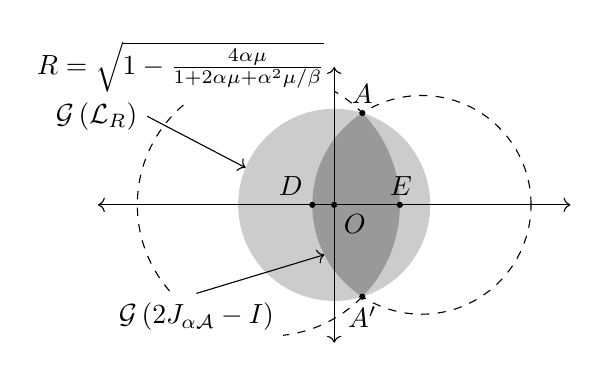
\begin{tikzpicture}[scale=2.5]
\def\m{0.5};
\def\b{.8};


\begin{scope}
\clip ({-\m/(1+\m)+sqrt(1/(1 + \m)/(1 + \m) + (4*\b*\m*(-1 + \b*\m))/(\b + \m + 2*\b*\m)/(\b + \m + 2*\b*\m))},-0.7)  rectangle (-1.2,.9);
\draw[dashed] ({-\m/(1+\m)},0) circle ({1-\m/(1+\m)});
\end{scope}

\begin{scope}
\clip ({-\m/(1+\m)+sqrt(1/(1 + \m)/(1 + \m) + (4*\b*\m*(-1 + \b*\m))/(\b + \m + 2*\b*\m)/(\b + \m + 2*\b*\m))},-.7)  rectangle (1.2,.9);
\draw[dashed] ({1/(1+1/\b)},0) circle ({1-1/(1+1/\b)});
\end{scope}



\draw (-.78,.7) node [fill=white] {$R=\sqrt{1-\frac{4\alpha\mu}{1+2\alpha\mu+\alpha^2\mu/\beta}}$};

\fill [fill=lightgrey] (0,0) circle ({sqrt((\b + \m - 2*\b*\m)/   (\b + \m + 2*\b*\m))});




\begin{scope}
\clip ({-\m/(1+\m)},0) circle ({1-\m/(1+\m)});
\fill[fill=medgrey] ({1/(1+1/\b)},0) circle ({1-1/(1+1/\b)});
%\draw[line width=1.0pt] ({1/(1+1/\b)},0) circle ({1-1/(1+1/\b)});
\end{scope}
\begin{scope}
\clip ({1/(1+1/\b)},0) circle ({1-1/(1+1/\b)});
%\draw[line width=1.0pt] ({-\m/(1+\m)},0) circle ({1-\m/(1+\m)});
\end{scope}
\draw [<->] (-1.2,0) -- (1.2,0);
\draw  [<->](0,-.7) -- (0,.7);

\coordinate (A) at  ({-\m/(1+\m)+sqrt(1/(1 + \m)/(1 + \m) + (4*\b*\m*(-1 + \b*\m))/(\b + \m + 2*\b*\m)/(\b + \m + 2*\b*\m))},{(2*sqrt(-(\b*\m*(-1 + \b*\m))))/(\b + \m + 2*\b*\m)}) ;
\coordinate (Ap) at  ({-\m/(1+\m)+sqrt(1/(1 + \m)/(1 + \m) + (4*\b*\m*(-1 + \b*\m))/(\b + \m + 2*\b*\m)/(\b + \m + 2*\b*\m))},{-(2*sqrt(-(\b*\m*(-1 + \b*\m))))/(\b + \m + 2*\b*\m)}) ;
\filldraw (A) circle ({0.6*1.5/2.5pt});
\draw (A) node[above] {$A$};
\filldraw (Ap) circle ({0.6*1.5/2.5pt});
\draw (Ap) node[below] {$A'$};


\filldraw ({(1-\m)/(1+\m)},0)circle ({0.6*1.5/2.5pt});
\draw ({(1-\m)/(1+\m)-0.1},0) node [above right] {$E$};
\filldraw ({(1-1/\b)/(1+1/\b)},0)circle ({0.6*1.5/2.5pt});
\draw ({(1-1/\b)/(1+1/\b)},0) node [above left] {$D$};

\draw (0,0) node [below right] {$O$};
\filldraw (0,0)circle ({0.6*1.5/2.5pt});


\def\x{-.05}
%\draw (-.1,-.9) node [below,fill=white] {$\cG\left(2\left(I+\alpha(\cM_\mu\cap \cC_\beta)\right)^{-1}-I\right)$};
\draw (-.7,-.45) node [below,fill=white] {$\cG\left(2J_{\alpha \cA}-I\right)$};
\draw [->] (-.7,-.45) -- (\x,{-sqrt(((2)/(2+2*\b))^2-(\x-2*(1+2*\b)/(2+2*\b)+1)^2)});

\def\y{-.45}
\draw [->] (-.95,.45) -- (\y,{sqrt((sqrt((\b + \m - 2*\b*\m)/   (\b + \m + 2*\b*\m)))^2-(\y)^2)});
%\draw (.4,.7) node [above,fill=white] {$\cG\left(\cL\left(\sqrt{1-\frac{4\alpha\mu}{1+2\alpha\mu+\alpha^2\mu/\beta}}\right)\right)$};
\draw (-.95,.45) node [left,] {$\cG\left(\cL_R\right)$};
\end{tikzpicture}}
\end{tabular}}
\end{center}
To clarify, $B$ is the center of the circle with radius $\overline{BA}$ and $C$ is the center of the circle with radius $\overline{CA}$.
\end{frame}


\begin{frame}
By Stewart's theorem, we have
\begin{align*}
\overline{OA}^2&=\frac{\overline{OC}\cdot \overline{AB}^2+\overline{BO}\cdot\overline{CA}^2-\overline{BO}\cdot\overline{OC}\cdot\overline{BC}}{\overline{BC}}\\
&=\frac{
\tfrac{\beta }{\alpha +\beta }\left(1-\tfrac{\alpha  \mu
   }{1+\alpha  \mu }\right)^2+
   \tfrac {\alpha  \mu } {1+\alpha \mu}
   \left (1 - \tfrac {\beta } {\alpha + \beta } \right)^2
   -\tfrac{\beta }{\alpha +\beta }
   \tfrac {\alpha  \mu } {1+\alpha \mu }
   \left(\tfrac{\beta }{\alpha +\beta}+\tfrac{\alpha  \mu }{1+\alpha  \mu }\right)
   }{\tfrac{\beta }{\alpha +\beta}+\tfrac{\alpha  \mu }{1+\alpha  \mu }}\\
&   =1-\frac{4\alpha\mu}{1+2\alpha\mu+\alpha^2\mu/\beta}.
\end{align*}
Since $2$ non-identitcal circles intersect at at most $2$ points, and since $D$ is within circle $B$, arc $\arc{ADA'}$ is within circle $O$.
By the same reasoning, 
%Since $2$ non-identitcal circles intersect at at most $2$ points, and since $E$ is within circle $A$,
arc $\arc{A'EA}$ is within circle $O$.
Finally, the region bounded by $\arc{ADA'}\cup \arc{A'EA}$ (darker shade) is within circle $O$ (lighter shade).
\vspace{0.2in}

The containment holds for $R$ and fails for smaller $R$.
Since $\cL_R$ is SRG-full by Theorem~\ref{thm:srg-full}, the containment of the SRG in $\ecomplex$ equivalent to the containment of the class.\qed
\end{frame}

\begin{frame}[plain,fragile]
\frametitle{Convergence analysis: DRS on optimization}
Consider
\[
\begin{array}{ll}
\underset{x\in \reals^n}{\mbox{minimize}}& f(x)+g(x),
\end{array}
\]
where $f$ and $g$ are CCP. Assume $f\in\cF_{\mu,L}$ or $g\in\cF_{0,\infty}$.
DRS
\begin{align*}
x^{k+1/2}&=\prox_{\alpha  g}(z^k)\\
x^{k+1}&=\prox_{\alpha  f}(2x^{k+1/2}-z^k)\\
z^{k+1}&=z^k+x^{k+1}-x^{k+1/2}
\end{align*}
converges exponentially with rate 
\begingroup\makeatletter\def\f@size{9}\check@mathfonts
\[
\|z^k-z^\star\|\le
\left(
\frac{1}{2}+\frac{1}{2}
\max\left\{
\left|\frac{1-\alpha\mu}{1+\alpha \mu}\right|,\left|\frac{1-\alpha L}{1+\alpha L}\right|
\right\}\right)^k
\|z^0-z^\star\|
\]
\endgroup
by the following Proposition~\ref{prop:refl-sm-coco} and Exercise~13.9.
\begin{proposition}
\label{prop:refl-cvx}
Let $0<\mu<L<\infty$ and $\alpha\in(0,\infty)$.
If $\cA= \partial \cF_{\mu,L}$, then 
$\opR_{\alpha \cA}\subseteq \cL_R$ for
\[
R=
\max\left\{
\left|\frac{1-\alpha\mu}{1+\alpha \mu}\right|,\left|\frac{1-\alpha L}{1+\alpha L}\right|
\right\}.
\]
Result is tight in the sense that $\opR_{\alpha \cA}\nsubseteq \cL_R$ for any smaller value of $R$.
\end{proposition}
\end{frame}


\begin{frame}[plain]
\textbf{Proof.}
By Theorems~\ref{thm:cvx-srg-first}, \ref{thm:srg-scaling-translation}, and \ref{thm:srg-inversion}, we have

\vspace{-0.15in}
\begin{center}
\begin{tabular}{ccccc}
\!\!\!\!\!\!
\raisebox{-.5\height}{
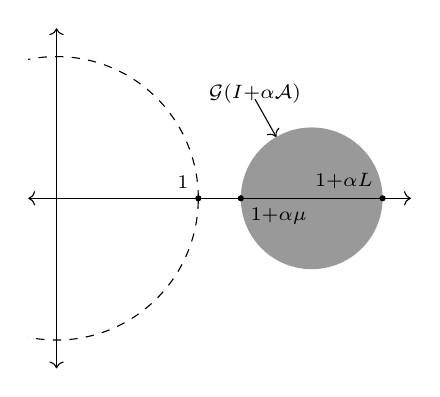
\begin{tikzpicture}[scale=1.8]
\def\m{0.3};
\def\L{1.3};

\draw (1.4,.6) node [above] {$\scriptstyle\cG\left(\opI+\alpha \cA\right)$};
\def\t{120};
\draw[->] (1.4,.7)--({(\L-\m)/2*cos(\t)+(2+\m+\L)/2},{(\L-\m)/2*sin(\t)});


\fill[fill=medgrey] ({(2+\m+\L)/2},0) circle ({(\L-\m)/2});
\begin{scope}
\clip (-0.2,-1.2) rectangle (2.5,1.2);
\draw [dashed] (0,0) circle (1);
\end{scope}

\draw [<->] (-0.2,0) -- (2.5,0);
\draw [<->] (0,-1.2) -- (0,1.2);
\draw (1,0)  node [above left] {$\scriptstyle 1$};
\filldraw (1,0) circle ({0.6*1.5/1.8pt});
\filldraw ({1+\L},0) circle ({0.6*1.5/1.8pt});
\draw ({1+\L},0)  node [above left] {$\scriptstyle 1+\alpha L$};
\draw ({1+\m},0)  node [below right] {$\scriptstyle 1+\alpha\mu$};
\filldraw ({1+\m},0) circle ({0.6*1.5/1.8pt});
\end{tikzpicture}
}
&\!\!\!\!\!\!
$\stackrel{\bar{z}^{-1}}{\longrightarrow}$
&\!\!\!\!\!\!
\raisebox{-.5\height}{
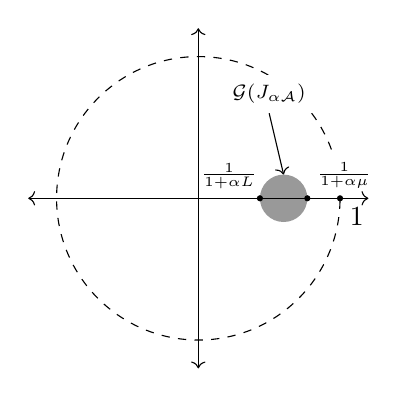
\begin{tikzpicture}[scale=1.8]
\def\m{0.3};
\def\L{1.3};

\draw [dashed] (0,0) circle (1);
\draw ({1/(1+\m)},0)  node [above right,fill=white] {$\scriptstyle\frac{1}{1+\alpha \mu}$};
\draw ({1/(1+\L)+.05},0)  node [above left, fill=white] {$\scriptstyle\frac{1}{1+\alpha L}$};


\draw (0.5,.6) node [above,fill=white] {$\scriptstyle\cG\left(\opJ_{\alpha \cA}\right)$};
\def\t{90};
\draw[->] (.5,.6)--({1/(1+\m)-1/(1+\L))/2*cos(\t)+(1/(1+\m)+1/(1+\L))/2},{1/(1+\m)-1/(1+\L))/2*sin(\t)});


\fill [fill=medgrey] ({(1/(1+\m)+1/(1+\L))/2},0) circle ({(1/(1+\m)-1/(1+\L))/2});
\draw [<->] (-1.2,0) -- (1.2,0);
\draw [<->] (0,-1.2) -- (0,1.2);

\filldraw ({1/(1+\L)},0) circle ({0.6*1.5/1.8pt});
\filldraw ({1/(1+\m)},0) circle ({0.6*1.5/1.8pt});
\draw (1,0)  node [below right] {$1$};
\filldraw (1,0) circle ({0.6*1.5/1.8pt});
\end{tikzpicture}}\\
&\!\!\!\!\!\!
$\stackrel{2z-1}{\longrightarrow}$
&\!\!\!\!\!\!\!\!\!\!\!\!\!\!\!\!\!\!\!\!\!\!\!\!\!\!\!\!\!\!\!\!\!
\!\!\!\!\!\!
\raisebox{-.5\height}{
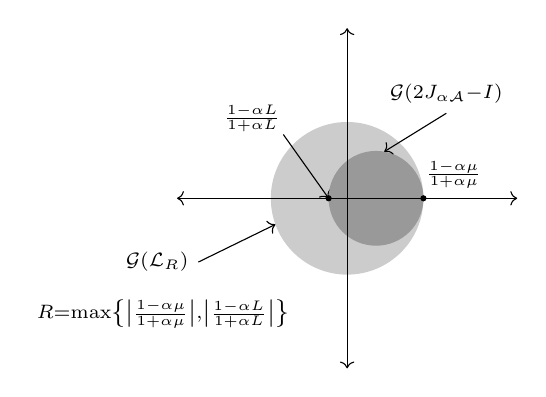
\begin{tikzpicture}[scale=1.8]
\def\m{0.3};
\def\L{1.3};
%\draw [dashed] (0,0) circle (1);
 
\draw (0.7,.6) node [above,fill=white] {$\scriptstyle\cG\left(2\opJ_{\alpha \cA}-\opI\right)$};
\draw (-1.3,-.65) node [below,fill=white] {$\scriptstyle R=\max\left\{\left|\frac{1-\alpha\mu}{1+\alpha \mu}\right|,\left|\frac{1-\alpha L}{1+\alpha L}\right|\right\}$};
\draw ({2/(1+\m)-1-0.05},0)  node [above right, fill=white] {$\scriptstyle\frac{1-\alpha \mu}{1+\alpha \mu}$};

\fill [fill=lightgrey] (0,0) circle ({(1-\m)/(1+\m)});

\draw[->] (-.45,.45)--({2/(1+\L)-1},0);

\draw (-.4,.4) node [above left] {$\scriptstyle\frac{1-\alpha L}{1+\alpha L}$};

\fill [fill=medgrey] ({(1/(1+\m)+1/(1+\L))-1},0) circle ({(1/(1+\m)-1/(1+\L))});
\draw [<->] (0,-1.2) -- (0,1.2);
\draw [<->] (-1.2,0) -- (1.2,0);
\filldraw ({2/(1+\L)-1},0) circle ({0.6*1.5/1.8pt});
\filldraw ({2/(1+\m)-1},0) circle ({0.6*1.5/1.8pt});
%\draw (1,0)  node [below right] {$1$};
%\filldraw (1,0) circle ({0.6*1.5/1.8pt});



\def\t{80}
\draw[->] (0.7,.6)--({(1/(1+\m)+1/(1+\L))-1+(1/(1+\m)-1/(1+\L))*cos(\t)},{(1/(1+\m)-1/(1+\L))*sin(\t)});
%\draw (0.4,.7) node [above, fill=white] {$\cG\left(2(I+\alpha \partial \cF_{\mu,L})^{-1}-I\right)$};

\def\s{200}
\draw[->] (-1.05,-.45)-- ({(1-\m)/(1+\m)*cos(\s)},{(1-\m)/(1+\m)*sin(\s)});


\draw (-1.05,-.45) node [left] {$\scriptstyle\cG\left(\cL_R\right)$};


\end{tikzpicture}
}
\end{tabular}
\end{center}
\end{frame}

\begin{frame}
The containment holds for $R$ and fails for smaller $R$.
Since $\cL_R$ is SRG-full by Theorem~\ref{thm:srg-full}, the containment of the SRG in $\ecomplex$ equivalent to the Since $\cL_R$ is SRG-full by Theorem~\ref{thm:srg-full}, the containment of the SRG in $\ecomplex$ equivalent to the containment of the class.
\qed
\end{frame}



\begin{frame}
%%%%%%%%%%%%%%%%%%%%%%%%%%%%%%%%%%%%%%%%
\frametitle{Sum of operators} 
%%%%%%%%%%%%%%%%%%%%%%%%%%%%%%%%%%%%%%%%
Lline segment between $z,w\in \complex$:
\[
[z,w]=\{\theta z+(1-\theta)w\,|\,\theta\in[0,1]\}.
\]
SRG-full class $\cA$ satisfies the chord property if $z\in \cG(\cA)\backslash\{\infty\}$ implies $[z,\bar{z}]\subseteq \cG(\cA)$.


\begin{center}
\begin{tabular}{c}
\raisebox{-.5\height}{
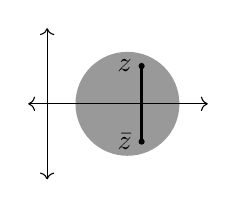
\begin{tikzpicture}[scale=1.2]
\fill[fill=medgrey] (0.85,0) circle (0.55);
\draw [<->] (-0.2,0) -- (1.7,0);
\draw [<->] (0,-.8) -- (0,.8);

\filldraw (1,.4) circle ({0.6*1.5/1.2pt});
\filldraw (1,-.4) circle ({0.6*1.5/1.2pt});
\draw [line width=1.0] (1,.4) -- (1,-.4);

\draw (1,.4) node [left] {$z$};
\draw (1,-.4) node [left] {$\bar{z}$};
\end{tikzpicture}
}
\end{tabular}
\end{center}

\begin{theorem}
\label{thm:srg-sum}
Let $\cA,\cB$ be SRG-full classes such that $\infty\notin \cG(A),\infty\notin \cG(B)$.
Then
\[
\cG(\cA+\cB)\supseteq \cG(\cA)+\cG(\cB).
\]
If $\cA$ or $\cB$ furthermore satisfies the chord property, then
\[
\cG(\cA+\cB)=\cG(\cA)+\cG(\cB).
\]
\vspace{-0.2in}
\end{theorem}
\end{frame}







\begin{frame}[plain]
\frametitle{Composition of operators}
Right-hand arc between $z\in \complex$ and $\bar{z}$:
\[
\rarc(z,\bar{z})
=\left\{re^{i(1-2\theta)\varphi}\,\Big|\,
z=re^{i\varphi},\,
\varphi\in(-\pi,\pi],\,\theta\in[0,1],\,r\ge 0
\right\}
\]
Left-hand arc between $z\in \complex$ and $\bar{z}$:
\[
\larc(z,\bar{z})
=-\rarc(-z,-\bar{z}).
%=\left\{re^{i\left(\theta|\varphi|+(1-\theta)(2\pi-|\varphi|)\right)}\,\Big|\,z=re^{i\varphi},\,|\varphi|\in[0,\pi],\,\theta\in[0,1],\,r\ge 0\right\}.
\]
\begin{center}
\begin{tabular}{cc}
\!\!\!\!\!\!\!\!\!\!\!\!\!\!\!
\raisebox{-.5\height}{
\begin{tikzpicture}[scale=1.6]
\def\x{0.5}
\fill[fill=medgrey] (-.4,0) circle (0.8);
\draw [<->] (-1.4,0) -- (0.7,0);
\draw [<->] (0,-1.) -- (0,1.);

\filldraw (.1,\x) circle[radius={0.6*1.5/1.5pt}];
\filldraw (.1,{-\x}) circle[radius={0.6*1.5/1.5pt}];
\begin{scope}
\clip (.1,-1.) rectangle (0.7,1.);
\draw [dashed] (0,0) circle ({sqrt(.1^2+\x^2)});
\end{scope}
\begin{scope}
\clip (-1.4,-1.) rectangle (0.1,1.);
\draw [line width=1.0] (0,0) circle (({sqrt(.1^2+\x^2)});
\end{scope}

\draw (.1,{\x}) node [above right] {$z$};
\draw (.1,{-\x}) node [below right] {$\bar{z}$};

\def\w{-.3}
\draw [->] (-0.75,-.8) -- (\w,{-sqrt(.1^2+\x^2-(\w)^2)});
\draw (-0.75,-.7)  node [below] {$\larc(z,\bar{z})$};
\end{tikzpicture}
}
&
\!\!\!\!\!\!\!\!\!\!\!\!\!\!\!\!\!\!
\raisebox{-.5\height}{
\begin{tikzpicture}[scale=1.1]
\fill[fill=medgrey] (0.85,0) circle (0.55);
\draw [<->] (-1.2,0) -- (1.6,0);
\draw [<->] (0,-1.4) -- (0,1.4);

\filldraw (1,.4) circle ({0.6*1.5/1pt});
\filldraw (1,-.4) circle ({0.6*1.5/1pt});
\begin{scope}
%\clip (-.3,-1.2) rectangle (1.6,1.2);
\draw [dashed] (0,0) circle ({sqrt(1+.4^2)});
\end{scope}
\begin{scope}
\clip (1,-1.2) rectangle (1.6,1.2);
\draw [line width=1.0] (0,0) circle ({sqrt(1+.4^2)});
\end{scope}

\draw (1,.4) node [left] {$z$};
\draw (1,-.4) node [left] {$\bar{z}$};

\def\w{1.05}
\draw [->] (-0.05,-.6) -- (\w,{sqrt(1+.4^2-\w^2)});
\draw (-0.05,-.6)  node [fill=white, left] {$\rarc(z,\bar{z})$};
\draw (-0,-.93)  node [below] {\phantom{$\larc(z,\bar{z})$}};
\end{tikzpicture}
}
\!\!\!\!\!\!\!\!\!
\end{tabular}
\end{center}

\vspace{0.2in}
An SRG-full class $\cA$ respectively satisfies the left-arc property and right-arc property
if $z\in \cG(\cA)\backslash\{\infty\}$
implies
$\larc{(z,\bar{z})}\subseteq \cG(\cA)$
and
$\rarc{(z,\bar{z})}\subseteq \cG(\cA)$, respectively.
$\cA$ satisfies \emph{an} arc property if the left or right-arc property is satisfied.
\end{frame}

\begin{frame}
\frametitle{Composition of operators}

\begin{theorem}
\label{thm:composition-srg}
Let $\cA$ and $\cB$ be SRG-full classes such that $\infty\notin \cG(\cA)$, $\emptyset\ne\cG(\cA)$, $\infty\notin \cG(\cB)$, and $\emptyset\ne \cG(\cB)$.
Then
\[
\cG(\cA\cB)\supseteq \cG(\cA)\cG(\cB).
\]
If $\cA$ or $\cB$ furthermore satisfies an arc property, then
\[
\cG(\cA\cB)=\cG(\cB\cA)=\cG(\cA)\cG(\cB).
\]
\end{theorem}
\end{frame}







\section{Averagedness coefficients}


\begin{frame}
\frametitle{Composition of averaged operators}
\begin{theorem}
\label{thm:avg-composition}
Let $\opT_1$ and $\opT_2$ be $\theta_1$- and $\theta_2$-averaged operators on $\reals^n$ with $\theta_1,\theta_2\in(0,1)$.
Then $\opT_1\opT_2$ is $\theta$-averaged with 
\[
\theta=\frac{\theta_1+\theta_2-2\theta_1\theta_2}{1-\theta_1\theta_2}.
\]
\vspace{-0.15in}
\end{theorem}
\end{frame}


\begin{frame}[plain,fragile]
\frametitle{Proof of Theorem~\ref{thm:avg-composition}}
% In the same vein as in Lemma~\ref{lem:avg-characterization},
Note
\[
z\in \cG(\cN_\theta)
\quad\Leftrightarrow\quad
|z-(1-\theta)|^2\le \theta^2
\quad\Leftrightarrow\quad
|z|^2\le 1-\frac{1-\theta}{\theta}|1-z|^2
\]
by Theorem~\ref{thm:monotone-srg} and 
\[
\theta^2-|z-(1-\theta)|^2
=\theta\left(
1-\frac{1-\theta}{\theta}|1-z|^2-|z|^2
\right).
\]
Let $z_1\in\cG(\cN_{\theta_1})$ and $z_2\in\cG(\cN_{\theta_2})$.
Then
\begingroup\makeatletter\def\f@size{9}\check@mathfonts
\begin{align*}
|z_1&z_2|^2\le 
|z_2|^2\left(
1-\frac{1-\theta_1}{\theta_1}|1-z_1|^2
\right)\\
&\le 
1-\frac{1-\theta_2}{\theta_1}|1-z_2|^2-\frac{1-\theta_1}{\theta_1}|1-z_1|^2|z_2|^2\\
&=
1-\frac{1-\theta}{\theta}|1-z_1z_2|^2-
\frac{\theta_1\theta_2}{\theta_1+\theta_2-2\theta_1\theta_2}
\left|
\frac{1-\theta_1}{\theta_1}(1-z_1)z_2-\frac{1-\theta_2}{\theta_2}(1-z_2)
\right|^2\\
&\le
1-\frac{1-\theta}{\theta}|1-z_1z_2|^2
\end{align*}
\endgroup
and $z_1z_2\in \cG(\cN_{\theta})$, i.e., $\cG(\cN_{\theta_1})\cG(\cN_{\theta_2})\subseteq \cG(\cN(\cG_\theta))$.
\end{frame}


\begin{frame}
\frametitle{Proof of Theorem~\ref{thm:avg-composition}}
%So $|z_1z_2|^2\le1-\frac{1-\theta}{\theta}|1-z_1z_2|^2$ implies
Since $\cN_{\theta_1}$ satisfies an arc property, $\cG(\cN_{\theta_1})\cG(\cN_{\theta_2})=\cG(\cN_{\theta_1}\cN_{\theta_2})$ by Theorem~\ref{thm:composition-srg}.
So 
\[
\cG(\cN_{\theta_1}\cN_{\theta_2})=\cG(\cN_{\theta_1})\cG(\cN_{\theta_2})\subseteq \cG(\cN_\theta),
\]
implies $\cN_{\theta_1}\cN_{\theta_2}\subseteq \cN_\theta$ by SRG-fullness of $\cN_\theta$.
\qed
\end{frame}

\begin{frame}[plain]
\frametitle{Alternate proof outline of Theorem~\ref{thm:avg-composition}}
$\mathcal{G}(\cN_{\theta_1})\cG(\cN_{\theta_2})$ is enclosed by the outer curve defined by
\[
r(\varphi)^2-2r(\varphi)(\cos(\varphi)(1-\theta_1)(1-\theta_2)+\theta_1\theta_2)+(1-2\theta_1)(1-2\theta_2)=0.
\]
\begin{figure}
\centering
\begin{subfigure}[b]{0.3\textwidth}
\vspace{-0.1in}
\raisebox{-.5\height}{
\begin{tikzpicture}[scale=1.5]
\begin{scope}
\clip (-0.1,-0.95) rectangle (0.1,0.95);
\end{scope}
\def\a{2/3};
\def\b{1/4};
\def\s{(\a+\b-2*\a*\b)/(1-\a*\b)};
\fill[fill=medgrey,samples=200,smooth] plot[domain=-180:180](\x:{cos(\x)*(1-\a)*(1-\b)+\a*\b+sqrt((cos(\x)*(1-\a)*(1-\b)+\a*\b)^2-(1-2*\a)*(1-2*\b))});
\draw[dashed] ({1-\s},0) circle ({\s});
\draw [<->] (-.65,0) -- (1.2,0);
\draw [<->] (0,-.85) -- (0,.85);
\draw (1,0)  node [above right] {1};
\filldraw (1,0) circle ({0.5*1.5/1.5pt});
\draw (0.3,-1) node [below] {$\theta_1=\frac{2}{3},\,\theta_2=\frac{1}{4}$};
\end{tikzpicture}
}
\end{subfigure}
\begin{subfigure}[b]{0.3\textwidth}
\vspace{-0.1in}
\raisebox{-.5\height}{
\begin{tikzpicture}[scale=1.5]
\begin{scope}
\clip (-0.1,-0.95) rectangle (0.1,0.95);
\end{scope}
\def\a{1/4};
\def\b{3/4};
\def\s{(\a+\b-2*\a*\b)/(1-\a*\b)};
\fill[fill=medgrey,samples=200,smooth] plot[domain=-180:180](\x:{cos(\x)*(1-\a)*(1-\b)+\a*\b+sqrt((cos(\x)*(1-\a)*(1-\b)+\a*\b)^2-(1-2*\a)*(1-2*\b))});
\draw[dashed] ({1-\s},0) circle ({\s});
\draw [<->] (-.65,0) -- (1.2,0);
\draw [<->] (0,-.85) -- (0,.85);
\draw (1,0)  node [above right] {1};
\filldraw (1,0) circle ({0.5*1.5/1.5pt});
\draw (0.3,-1) node [below] {$\theta_1=\frac{1}{4},\,\theta_2=\frac{3}{4}$};
\end{tikzpicture}
}
\end{subfigure}
\begin{subfigure}[b]{0.3\textwidth}
\vspace{-0.1in}
\raisebox{-.5\height}{
\begin{tikzpicture}[scale=1.5]
\begin{scope}
\clip (-0.1,-0.95) rectangle (0.1,0.95);
\end{scope}
\def\a{2/3};
\def\b{3/4};
\def\s{(\a+\b-2*\a*\b)/(1-\a*\b)};
\fill[fill=medgrey,samples=200,smooth] plot[domain=-180:180](\x:{cos(\x)*(1-\a)*(1-\b)+\a*\b+sqrt((cos(\x)*(1-\a)*(1-\b)+\a*\b)^2-(1-2*\a)*(1-2*\b))});
\draw[dashed] ({1-\s},0) circle ({\s});
\draw [<->] (-.75,0) -- (1.2,0);
\draw [<->] (0,-.9) -- (0,.9);
\draw (1,0)  node [above right] {1};
\filldraw (1,0) circle ({0.5*1.5/1.5pt});
\draw (0.3,-1) node [below] {$\theta_1=\frac{2}{3},\,\theta_2=\frac{3}{4}$};
\end{tikzpicture}
}
\end{subfigure}
\begin{subfigure}[b]{0.3\textwidth}
\vspace{-0.1in}
\raisebox{-.5\height}{
\begin{tikzpicture}[scale=1.5]
\begin{scope}
\clip(0.1,-1.05) rectangle (0.3,1.05);
\end{scope}
\def\t{0.25};
\def\s{2/5};
\fill[fill=medgrey,samples=200,smooth] plot[domain=-180:180](\x:{2*\t*(1-\t)+2*\t^2*cos(\x)});
\draw[dashed] ({2*\t-\s},0) circle (\s);
\draw [<->] (-0.2-1+2*\t,0) -- (1.2-1+2*\t,0);
\draw [<->] (-1+2*\t,-.7) -- (-1+2*\t,.7);
\draw (2*\t,0)  node [above right] {1};
\filldraw (2*\t,0) circle ({0.5*1.5/1.5pt});
\draw (2*\t^2-3*\t+0.5,-1) node [below] {$\theta_1=\theta_2=\frac{1}{4}$};
\end{tikzpicture}
}
\end{subfigure}
\begin{subfigure}[b]{0.3\textwidth}
\vspace{-0.1in}
\raisebox{-.5\height}{
\begin{tikzpicture}[scale=1.5]
\begin{scope}
\clip(0.1,-1.05) rectangle (0.3,1.05);
\end{scope}
\def\s{1/1.5};
\fill[fill=medgrey,samples=200,smooth] plot[domain=-180:180](\x:{1/2+1/2*cos(\x)});
\draw[dashed] ({1-\s},0) circle ({\s});
\draw [<->] (-.5,0) -- (1.2,0);
\draw [<->] (0,-.7) -- (0,.7);
\draw (1,0)  node [above right] {1};
\filldraw (1,0) circle ({0.5*1.5/1.5pt});
\draw (0.35,-1) node [below] {$\theta_1=\theta_2=\frac{1}{2}$};
\end{tikzpicture}
}
\end{subfigure}
\begin{subfigure}[b]{0.3\textwidth}
\vspace{-0.1in}
\raisebox{-.5\height}{
\begin{tikzpicture}[scale=1.5]
\begin{scope}
\clip(0.1,-1.05) rectangle (0.3,1.05);
\end{scope}
\def\t{0.75};
\def\s{(2*\t)/(1+\t)};
\fill[fill=medgrey,samples=200,smooth] plot[domain=-180:180](\x:{2*\t*(1-\t)+2*\t^2*cos(\x)});
\draw[dashed] ({2*\t-\s},0) circle ({\s});
\draw [<->] (-0.8-1+2*\t,0) -- (1.2-1+2*\t,0);
\draw [<->] (-1+2*\t,-1) -- (-1+2*\t,1);
\draw (2*\t,0)  node [above right] {1};
\filldraw (2*\t,0) circle ({0.5*1.5/1.5pt});
\draw (2*\t^2-2*\t+1,-1) node [below] {$\theta_1=\theta_2=\frac{3}{4}$};
\end{tikzpicture}
}
\end{subfigure}
\end{figure}
\end{frame}

\begin{frame}
\frametitle{Alternate proof outline of Theorem~\ref{thm:avg-composition}}
The disk $\cG(\cN_\theta)$ with 
$\theta=\frac{\theta_1+\theta_2-2\theta_1\theta_2}{1-\theta_1\theta_2}$
contains this region so $\cG(\cN_{\theta_1})\cG(\cN_{\theta_2})\subseteq \cG(\cN_\theta)$.
On the other hand, the two shapes have matching curvature at $1$, the inclusion does not hold with smaller $\theta$.
\qed
\end{frame}


\begin{frame}
\frametitle{Davis--Yin splitting}
\begin{theorem}
\label{thm:dys_conv}
Assume $\opA$, $\opB$, and $\opC$ are maximal monotone. Assume $\opC$ is $\beta$-cocoercive and $\alpha\in (0,2\beta)$.
The DYS operator $\opI -\opJ_{\alpha \opB}+\opJ_{\alpha \opA}(\opR_{\alpha \opB}-\alpha \opC \opJ_{\alpha \opB})$
is $\theta$-averaged with
\[
\theta=\frac{2\beta}{4\beta-\alpha}.
\]
\vspace{-0.2in}
\end{theorem}
\end{frame}

\begin{frame}
\frametitle{Proof of Theorem~\ref{thm:dys_conv}}
\setcounter{theorem}{4}
\begin{lemma}
\label{lem:avg-characterization}
For $\theta\in(0,1)$, $\opT$ is $\theta$-averaged if and only if
\[
\|\opT x-\opT y\|^2\le\|x-y\|^2-\frac{1-\theta}{\theta}\|\opT x-x-\opT y+y\|^2\qquad\forall,\,x,y\in\reals^n.
\]
\end{lemma}
\textbf{Proof.}
Note $\opT$ is $\theta$-averaged if and only if $\frac{1}{\theta}\opT -\left(\frac{1}{\theta}-1\right)\opI$ is nonexpansive.
The claim follows from
\begin{align*}
0&\ge
\left\|\frac{1}{\theta}\opT x-\left(\frac{1}{\theta}-1\right)x
-\frac{1}{\theta}\opT y+\left(\frac{1}{\theta}-1\right)y
\right\|^2-\|x-y\|^2\\
&=
\frac{1}{\theta}
\left(
\|\opT x-\opT y\|^2+\frac{1-\theta}{\theta}\|\opT x-x-\opT y+y\|^2-\|x-y\|^2
\right).
\end{align*}
\qed
\end{frame}

\begin{frame}[fragile]
\frametitle{Proof of Theorem~\ref{thm:dys_conv}}
%[Proof of Theorem~\ref{thm:dys_conv}]
For any $z^0,\hat{z}^0\in \mathbb{R}^n$, let
\begin{center}
\begin{tabular}{l|l}
\parbox{0.3\linewidth}{%
\begin{align*}
x^{1/2}&=\opJ_{\alpha \opB}(z^0)\\
x^{1}&=\opJ_{\alpha \opA}(2x^{1/2}-z^k-\alpha \opC x^{1/2})\\
z^{1}&=z^0+x^{1}-x^{1/2}
\end{align*}}
&
\parbox{0.3\linewidth}{%
\begin{align*}
\hat{x}^{1/2}&=\opJ_{\alpha \opB}(\hat{z}^0)\\
\hat{x}^{1}&=\opJ_{\alpha \opA}(2\hat{x}^{1/2}-\hat{z}^k-\alpha \opC \hat{x}^{1/2})\\
\hat{z}^{1}&=\hat{z}^0+\hat{x}^{1}-\hat{x}^{1/2}.
\end{align*}}
\end{tabular}
\end{center}
Define
\begingroup\makeatletter\def\f@size{9}\check@mathfonts
\begin{center}
\begin{tabular}{l|l}
\parbox{0.45\linewidth}{%
\begin{align*}
\tilde{\opB}x^{1/2}&=\frac{1}{\alpha}(z^0-x^{1/2})\\
\tilde{\opA}x^{1}&=\frac{1}{\alpha}(2x^{1/2}-z^k-\alpha \opC x^{1/2}-x^{1})
\end{align*}}
&
\parbox{0.45\linewidth}{%
\begin{align*}
\tilde{\opB}\hat{x}^{1/2}&=\frac{1}{\alpha}(\hat{z}^0-\hat{x}^{1/2})\\
\tilde{\opA}\hat{x}^{1}&=\frac{1}{\alpha}(2\hat{x}^{1/2}-\hat{z}^k-\alpha \opC \hat{x}^{1/2}-\hat{x}^{1}),
\end{align*}}
\end{tabular}
\end{center}
\endgroup
\end{frame}



\begin{frame}[plain]
\frametitle{Proof of Theorem~\ref{thm:dys_conv}}
which implies
\begin{center}
\begin{tabular}{l|l}
\parbox{0.3\linewidth}{%
\begin{align*}
\tilde{\opB}x^{1/2}&\in\opB x^{1/2}\qquad
\\
\tilde{\opA}x^{1}&\in \opA x^{1}
\end{align*}}
&
\parbox{0.3\linewidth}{%
\begin{align*}
\tilde{\opB}\hat{x}^{1/2}&\in \opB \hat{x}^{1/2}
\\
\tilde{\opA}\hat{x}^{1}&\in \opA \hat{x}^{1}.
\end{align*}}
\end{tabular}
\end{center}
Then
\begin{align*}
\|z^{1}-\hat{z}^1\|^2&=\|z^{0}-\hat{z}^0\|^2-\frac{1-\theta}{\theta}\|z^{1}-z^0-\hat{z}^1+\hat{z}^0\|^2\\
&
-2\alpha\langle\tilde{\opA} x^{1}-\tilde{\opA} \hat{x}^{1},x^{1}-\hat{x}^{1}\rangle
-2\alpha\langle\tilde{\opB} x^{1/2}-\tilde{\opB} \hat{x}^{1/2},x^{1/2}-\hat{x}^{1/2}\rangle
\\
&-2\alpha\left(\langle\opC x^{1/2}-\opC \hat{x}^{1/2},x^{1/2}-\hat{x}^{1/2}\rangle-\beta\|\opC x^{1/2}-\opC \hat{x}^{1/2}\|^2\right)\\
&-\frac{\alpha^2}{2\beta}\left\|\tilde{\opA} x^{1}-\tilde{\opA} \hat{x}^{1}+\tilde{\opB} x^{1/2}-\tilde{\opB} \hat{x}^{1/2}-\frac{2\beta-\alpha}{\alpha}(\opC x^{1/2}-\opC \hat{x}^{1/2})\right\|^2\\
&\le\|z^{0}-\hat{z}^0\|^2-\frac{1-\theta}{\theta}\|z^{1}-z^0-\hat{z}^1+\hat{z}^0\|^2,
\end{align*}
where the inequality follows from monotonicity of $\opA$ and $\opB$ and $\beta$-cocoercivity of $\opC$.
Finally, the claim follows from Lemma~\ref{lem:avg-characterization}.\qed
\end{frame}


\begin{frame}
\frametitle{SRG of DYS}
Let 
\[
\cT_{\alpha,\beta}=\{\opI -\opJ_{\alpha \opB}+\opJ_{\alpha \opA}(\opR_{\alpha \opB}-\alpha \opC \opJ_{\alpha \opB})\,|\,\opA,\opB\in \cM,\,\opC\in\cC_\beta\}.
\]
be the class of DYS operators. 
Theorem~\ref{thm:dys_conv} states $\cG(\cT_{\alpha,\beta})\subseteq\cG\Big(\cN_{\frac{2\beta}{4\beta-\alpha}}\Big)$ for $\alpha\in(0,2\beta)$
One can furthermore show
\[
\cG(\cT_{\alpha,\beta})=\cG\left(\cN_{\frac{2\beta}{4\beta-\alpha}}\right)=
\hspace{-0.1in}
\begin{tabular}{c}
\raisebox{-.5\height}{
\begin{tikzpicture}[scale=1.8]

% b_i=1/beta_i
\def\b{1};
\def\c{1};
\def\g{1.3};
\def\gg{1};
\def\t{18};

\coordinate (O) at (0,0);
\coordinate (A) at ({cos(\t)^2},{cos(\t)*sin(\t)});
\coordinate (X) at (1,0);
\coordinate (I) at ({1-2\b*\c/(4-\g)},0);
\coordinate (A_2) at ({1-\b*\c+\b*\c*cos(2*\t)^2},{\b*\c*cos(2*\t)*sin(2*\t)});
\coordinate (O_4) at ({1-\b*\c+\b*\c*(cos(2*\t)-\g/2*cos(\t)^2)*cos(2*\t)},{\b*\c*(cos(2*\t)-\g/2*cos(\t)^2)*sin(2*\t)});
\coordinate (A_3) at ({\g*\b*\c*cos(\t)^2*(cos(2*\t))},{\g*\b*\c*cos(\t)^2*(sin(2*\t))});
\coordinate (O_3) at ({0.5*\g*\b*\c*cos(\t)^2*(cos(2*\t))},{0.5*\g*\b*\c*cos(\t)^2*(sin(2*\t))});
\coordinate (I) at ({1-2*\b*\c/(4-\g)},0);
\coordinate (II) at ({1-2*\b*\c/(4-\gg)},0);
\coordinate (B) at (-0.13,0.63);
\coordinate (T) at (0.99,0.41);
\coordinate (T') at (-0.34,0.06);


\fill [medgrey] (I) circle ({2*\b*\c/(4-\g)});


\draw [<->] (-0.6,0) -- (1.2,0);
\draw [<->] (0,-0.8) -- (0,0.8);

\filldraw (X) circle[radius={0.5*1.5/1.8pt}];
\filldraw (I) circle[radius={0.5*1.5/1.8pt}];


\draw (X) node[above right] {$1$};
\draw (0.25,0) node[below] {$\frac{2\beta-\alpha}{4\beta-\alpha}$};

% \draw (0.85,0.65) node[above] {$\partial \Avc\left(\frac{2\beta}{4\beta-\alpha}\right)$};
% \draw [->] (0.9,0.7) -- (0.75,0.555);

\end{tikzpicture}}
\end{tabular}
\]
\end{frame}






\section{Proofs of SRG theorems}



\begin{frame}
\frametitle{Operator from SRG}

$\cG(\cdot)$ maps $\opA$ to a subset of $\ecomplex$.
Below conversely maps $z$ to $\opA_z$ such that $z\in \cG(\opA_z)$.
%Lemma~\ref{lem:complex-srg} provides such constructions.
%the construction of operators that correspond a given point in $\ecomplex$.
%We omit the proofs as they follow from definitions and basic computation.
\setcounter{theorem}{3}
\begin{lemma}
\label{lem:complex-srg}
Take any $z=z_r+z_ii\in \complex$. 
Define
$\opA_z\colon\reals^2\rightarrow\reals^2$
and $\opA_\infty\colon\reals^2\rightrightarrows\reals^2$ as
\[
\opA_z\begin{bmatrix}
\zeta_1\\\zeta_2
\end{bmatrix}
=
\begin{bmatrix}
z_r\zeta_1-z_i\zeta_2\\
z_r\zeta_2+z_i\zeta_1
\end{bmatrix}
\qquad
\opA_\infty(x)=\left\{
\begin{array}{ll}
\reals^2&\text{if }x=0\\
\emptyset&\text{otherwise.}
\end{array}
\right.
\]
Then, 
\[
\mathcal{G}(\opA_z)=\{z,\bar{z}\},
\qquad
\mathcal{G}(\opA_\infty)=\{\infty\}.
\]
\end{lemma}
If $\cong$ identifies $\mathbb{R}^2$ with $\mathbb{C}$,
\[
\begin{bmatrix}
x\\y
\end{bmatrix}
\cong x+yi,
\]
then $\opA_z$ is complex multiplication with $z$:
\[
\opA_z\begin{bmatrix}
\zeta_1\\\zeta_2
\end{bmatrix}
\cong z(\zeta_1+\zeta_2i).
\]
\end{frame}


\begin{frame}
\frametitle{Proof of Lemma~\ref{lem:complex-srg}}
%\textbf{Proof of Lemma~\ref{lem:complex-srg}.}
%Again, we write $\cong$ to identify an element of $\mathbb{R}^2$ with an element in $\mathbb{C}$.
Write $z=r_ze^{i\theta_{z}}$.
Consider any $x,y\in \reals^2$ where $x\ne y$ and define $u=\opA_zx$ and $v=\opA_zy$.
Then we can write
\[
x-y=r_w
\begin{bmatrix}
\cos(\theta_w)\\
\sin(\theta_w)
\end{bmatrix}
\]
where $r_w>0$, and
\[
u-v=\opA_z(x-y)\cong r_{z}r_we^{i(\theta_{z}+\theta_w)}.
\]
This gives us
\[
\frac{\|u-v\|}{\|x-y\|}= r_z,\quad
\quad
\angle (u-v,x-y)=|\theta_z|,
\quad
\cG(\opA_z)=\left\{r_{z}e^{i\theta_{z}},r_{z}e^{- i\theta_{z}}\right\}.
\]
% Now we let 
% $x-y=r_we^{i\theta_w}$, and $u-v=r_{z}r_we^{i(\theta_{z}+\theta_w)}$, (note that $x+yi$ is a linear operator) we get
\vspace{0.2in}

Now consider $\opA_\infty$.
By definition, $\infty\in \cG(\opA_\infty)$.
For any $u\in \opA_\infty x$ and $v\in \opA_\infty y$, we have $x=y=0$,
and therefore $\cG(\opA_\infty)$ contains no finite $z\in \complex$.
We conclude $\cG(\opA_\infty)=\{\infty\}$.
%Since $\dom (A_\infty)=\{0\}$, 
\qed
\end{frame}




\begin{frame}
%\frametitle{SRG of operator classes}
\frametitle{Proof of Theorem~\ref{thm:monotone-srg}}
%We prove the characterizations of $\cG(\cL_L)$ and $\cG(\cM)$.
%Although we can characterize  $\cG(\cM_\mu)$, $\cG(\cC_\beta)$, and $\cG(\cN_\theta)$ with similar direct proofs, we provide simpler proofs later in \S\ref{ss:srg-classes-proofs} that use operator and SRG transformations.
%First, characterize $\cG(\cL_L)$.
%We have $\cG(\cL_L)\subseteq\left\{z\in \complex\,\big|\,|z|^2\le L^2\right\}$ since
%\[
%\opA\in \cL_L
%\;\;\Rightarrow\;\;
%\frac{\|\opA x-\opA y\|}{\|x-y\|}\le L,\,\forall\,x,y\in \reals^n,\,x\ne y
%\;\;\Rightarrow\;\;
%\cG(\opA)\subseteq\left\{z\in \complex\,\big|\,|z|^2\le L^2\right\}.
%\]
%Conversely, given any $z\in \complex$ such that $|z|\le L$, the operator $\opA_z$ of Lemma~\ref{lem:complex-srg} satisfies $\|\opA_zx-\opA_zy\|\le L\|x-y\|$ for any $x,y\in \reals^2$, i.e., $\opA_z\in \cL_L$, and $\cG(\opA_z)=\{z,\bar{z}\}$. Therefore
%$\cG(\cL_L)\supseteq \left\{z\in \complex\,\big|\,|z|^2\le L^2\right\}$.% and we have equality.
% The proof has 2 parts: that the SRG is contained in the region and that the SRG fills the entire region.
% Since the left-hand side and the right-hand wide both include $\infty$, we only need to consider the finite points.
%First, we show $\cG(\cM)\backslash\{\infty\}\subseteq \{z\,|\,\Re z\ge 0\}$.
Characterize $\cG(\cM)$.
For any $\opA\in \cM$,
\[
\Re z=\frac{\langle u-v,x-y\rangle}{\|x-y\|^2}\ge 0,
\quad\forall\,u\in \opA x,\,v\in \opA y,\,x\ne y.
\]
(Cf.\ page~\pageref{slide_srg_op}.)
Therefore, $\cG(\opA)\backslash\{\infty\}\subseteq \{z\,|\,\Re z\ge 0\}$.
%Next, we show $\{z\,|\,\Re z\ge 0\}\subseteq \cG(\mathcal{M})$.
On the other hand, given any $z\in \{z\,|\,\Re z\ge 0\}$, the operator $\opA_z$ of Lemma~\ref{lem:complex-srg} satisfies $\langle \opA_zx-\opA_zy,x-y\rangle \ge 0$ for any $x,y\in \reals^2$, i.e., $\opA_z\in \cM$, and $\cG(\opA_z)=\{z,\bar{z}\}$.
Therefore, $z\in\cG(\opA_z)\subset \cG(\cM)$, and we conclude $\{z\,|\,\Re z\ge 0\}\subseteq \cG(\mathcal{M})$.
Finally, note that $\infty\in \cG(\cM)$ is equivalent to saying that there exists a multi-valued operator in $\cM$.
The $\opA_\infty$ of Lemma~\ref{lem:complex-srg} is one such example.
%This proves equality.
\vspace{0.2in}

The other SRGs follow from a similar reasoning.
%We leave the characterization of $\cG(\cM_\mu)$, $\cG(\cC_\beta)$, and $\cG(\cN_\theta)$ to Exercise~\ref{exercise:srgthm}.
\qed
\end{frame}





\begin{frame}
%\frametitle{SRG of subdifferential operators}
\frametitle{Proof outline of Theorem~\ref{thm:cvx-srg-first}}
%The proof has 2 parts: that the SRG is contained in the region and that the SRG fills the entire region.
$\partial \mathcal{F}_{0,\infty}\subset \mathcal{M}$ and Theorem~\ref{thm:monotone-srg}
 implies $\cG(\partial \mathcal{F}_{0,\infty})\subseteq\cG(\cM)= \{z\in\complex\,|\,\Re z\ge 0\}\cup\{\infty\}$.
 
 \vspace{0.2in}
With basic computation, we can verify $f\colon\reals^2\rightarrow\reals$ defined by $f(x,y)=|x|$ satisfies $\cG(\partial f)=\{z\in\complex\,|\,\Re z\ge 0\}\cup\{\infty\}$. This tells us $\{z\in\complex\,|\,\Re z\ge 0\}\cup\{\infty\}\subseteq\cG(\partial \mathcal{F}_{0,\infty})$.

%\vspace{0.2in}
%
%We prove the claim with basic computation.
%Let $f(x,y)=|x|$.
%The subgradient has the form $\partial f(x,y)=(h(x),0)$ for $h$ defined by:
%\[
%h(x) =
%\left\{
%\begin{array}{ll}
%\{-1\}&\text{for }x<0\\
%\{u\,|\,-1\le u\le 1\}&\text{for }x=0\\
%\{1\}&\text{for }x>0.
%\end{array}\right.
%\]
%Since $\partial f$ is multi-valued at $(0,0)$, we have $\infty\in \cG(\partial f)$. 
%Since $\partial f(1,0)=\partial f(2,0)$, we have $0\in \cG(\partial f)$. 
%The input-output pairs
%$(0,0)\in \partial f(0,0)$ and $(h(R\cos(\theta)),0)\in\partial f(R\cos(\theta),R\sin(\theta))$ map to the point $R^{-1}(|\cos(\theta)|,\pm\sin(\theta))\in\CC$. Clearly the image of this map over the range $R\in(0,\infty)$, $\theta\in[0,2\pi)$ is the right-hand plane except the origin. Hence $\cG(\partial f)=\{z\in\complex\,|\,\Re z\ge 0\}\cup\{\infty\}$.

\vspace{0.2in}
The other SRGs follow from a similar reasoning.
\qed
\end{frame}

\begin{frame}
\frametitle{Proof of Theorem~\ref{thm:srg-full}}

\end{frame}

\begin{frame}
\frametitle{Proof of Theorem~\ref{thm:srg-intersection}}
Since $\cA$ and $\cB$ are SRG-full
\begin{align*}
\cG(\opC)\subseteq\cG(\cA\cap\cB)\subseteq \cG(\cA)\cap \cG(\cB)
\quad&\Rightarrow\quad \cG(\opC)\subseteq \cG(\cA)\text{ and }\cG(\opC)\subseteq \cG(\cB)\\
\quad&\Rightarrow\quad \opC\in \cA\text{ and }\opC\in \cB\\
\quad&\Rightarrow\quad \opC\in \cA\cap \cB
\end{align*}
for an operator $\opC$, 
and we conclude $\cA\cap\cB$ is SRG-full.
\vspace{0.2in}


%Since $A\in \cA$ if and only if $\cG(A)\subseteq \cG(\cA)$ and $B\in \cB$ if and only if $\cG(B)\subseteq \cG(\cB)$, we have
Assume $z\in\complex$ satisfies $\{z,\bar{z}\}\subseteq \cG(\cA)\cap \cG(\cB)$.
Then $\opA_z$ of Lemma~\ref{lem:complex-srg} satisfies $\cG(\opA_z)=\{z,\bar{z}\}\subseteq \cG(\cA)\cap \cG(\cB)$.
Since $\cA$ and $\cB$ are SRG-full, $\opA_z\in \cA$ and $\opA_z\in \cB$
and $\{z,\bar{z}\}=\cG(\opA_z)\subseteq \cG(\cA\cap \cB)$.
If $\infty\in \cG(\cA)\cap \cG(\cB)$, then
a similar argument using $\opA_\infty$ of Lemma~\ref{lem:complex-srg} proves $\infty \in \cG(\cA\cap \cB)$.
Therefore $\cG(\cA)\cap \cG(\mathcal{B})\subseteq \cG(\cA\cap \mathcal{B})$.
Since the other containment $\cG(\cA\cap \mathcal{B})\subseteq \cG(\cA)\cap \cG(\mathcal{B})$ holds by definition, we have the equality.
\qed
\end{frame}

\begin{frame}
\frametitle{Proof of Theorem~\ref{thm:srg-scaling-translation}}
 $\cG(\alpha \opA)=\alpha\cG(\opA)$ follows from the definition of the SRG, and 
 $\cG(\opI+ \opA)=1+\cG(\opA)$ follows from  
\[
\Re z
=\frac{\langle u-v,x-y\rangle}{\|x-y\|^2},
\qquad
\Im z
=\pm
\frac{\|P_{\{x-y\}^\perp}(u-v)\|}{\|x-y\|}.
%=\pm\frac{1}{\|x-y\|}\sqrt{\|u-v\|^2-\frac{(\langle u-v,x-y\rangle)^2}{\|x-y\|^2}},
\]
% The statements with the operator classes follow from the statements with the individual operators and from the definition of the SRG of operator classes.
The scaling and translation operations are reversible and $\cG((1/\alpha)\cA)=(1/\alpha)\cG(\cA)$ and $\cG(\cA-\opI)=\cG(A)-1$.
For any $\opB\colon\reals^n\rightrightarrows\reals^n$,
\[
\cG(\opB)\subseteq \cG(\alpha \cA)
\,\,\Rightarrow\,\,
\cG((1/\alpha)\opB)\subseteq \cG(\cA)
\,\,\Rightarrow\,\,
(1/\alpha)\opB\in \cA
\,\,\Rightarrow\,\,
\opB\in\alpha \cA,
\]
and we conclude $\alpha \cA$ is SRG-full.
By a similar reasoning,  $\opI+ \cA$ is SRG-full.
\qed
% To clarify, $\alpha\cG(\opA)$ corresponds to scaling $\cG(\opA)\subseteq \ecomplex$ by $|\alpha|$ and reflecting about the vertical axis (imaginary axis) if $\alpha<0$.
%Remember that $\cG(A)$ is symmetric about the horizontal axis (real axis).
%Again, $A\alpha $ is the operator defined by $x\mapsto A(\alpha x)$.
%We require $\alpha\ne 0$ to avoid $0\cdot\infty$.
%To clarify, $1\in \complex$ and $1+\cG(A)$ corresponds to shifting $\cG(A)$ to the right by one unit.
\end{frame}



\begin{frame}[fragile]
\frametitle{Proof of Theorem~\ref{thm:srg-inversion}}
The equivalence of non-zero finite points, i.e.,
\[
\cG(\opA^{-1})\backslash\{0,\infty\}=\left(\cG(\opA)\right\backslash\{0,\infty\})^{-1},
\]
follows from
\begingroup\makeatletter\def\f@size{9}\check@mathfonts
\begin{align*}
\!\!\!\!\!\!
\mathcal{G}(\opA)\backslash\{0,\infty\}&=
\left\{
\frac{\|u-v\|}{\|x-y\|}
\exp\left[\pm i \angle (u-v,x-y)\right]
\,\Big|\,
(x,u),(y,v)\in \opA,\, x\ne y,\,u\ne v \right\}
\end{align*}
\endgroup
and
\begin{align*}
&\!\!\!\!\mathcal{G}(\opA^{-1})\backslash\{0,\infty\}\\
&=
\left\{
\frac{\|x-y\|}{\|u-v\|}
\exp\left[\pm i \angle (x-y,u-v)\right]
\,\Big|\,
(u,x),(v,y)\in \opA^{-1},\, x\ne y,\,u\ne v \right\}\\
&=
\left\{
\frac{\|x-y\|}{\|u-v\|}
\exp\left[\pm i \angle (u-v,x-y)\right]
\,\Big|\,
(x,u),(y,v)\in \opA,\, x\ne y,\,u\ne v \right\}\\
&=\left(\cG(\opA)\backslash\{0,\infty\}\right)^{-1}.
\end{align*}
% $(x,u)\in A$ if and only if $(u,x)\in A^{-1}$
% and the fact that
\end{frame}

\begin{frame}
\frametitle{Proof of Theorem~\ref{thm:srg-inversion}}
The equivalence of the zero and infinite points follow from
\begin{align*}
\infty\in \cG(\opA)
&\quad\Leftrightarrow\quad
\exists\, (x,u),(x,v)\in \opA,\,u\ne v\\
&\quad\Leftrightarrow\quad
\exists\, (u,x),(v,x)\in \opA^{-1},\,u\ne v\\
&\quad\Leftrightarrow\quad
0\in \cG(\opA^{-1}).
\end{align*}
With the same argument, we have
$0\in \cG(\opA)
\Leftrightarrow
\infty\in \cG(\opA^{-1})$.
\vspace{0.2in}


The inversion operation is reversible.
Therefore, for any $\opB\colon\reals^n\rightrightarrows\reals^n$,
\[
\cG(\opB)\subseteq \cG( \cA^{-1})
\,\,\Rightarrow\,\,
\cG(\opB^{-1})\subseteq \cG(\cA)
\,\,\Rightarrow\,\,
\opB^{-1}\in \cA
\,\,\Rightarrow\,\,
\opB\in\cA^{-1},
\]
and we conclude $\cA^{-1}$ is SRG-full.\qed
\end{frame}

\begin{frame}
\frametitle{Proof of Theorem~\ref{thm:srg-sum}}

\end{frame}


\begin{frame}
\frametitle{Spherical triangle inequality}
Spherical triangle inequality: $|\theta-\varphi|\le \psi\le \theta+\varphi$
\begin{center}
\includegraphics[width=0.5\textwidth]{spherical_triangle.png}
\end{center}

%\vspace{0.2in}
For any nonzero $a,b,c\in \reals^n$,
\[\left|\angle (a,b)-\angle (b,c)\right|
\le \angle (a,c)\le 
%\max\left\{ \angle (a,b)+\angle (b,c),\pi/2\right\}
 \angle (a,b)+\angle (b,c).
\]
\end{frame}




\begin{frame}
\frametitle{Proof of Theorem~\ref{thm:composition-srg}}
We first show $\cG(\cA\cB)\supseteq \cG(\cA)\cG(\cB)$.
Assume $\cG(\cA)\ne \emptyset$ and $\cG(\cB)\ne \emptyset$ as otherwise there is nothing to show.
Let $z\in \cG(\cA)$ and $w\in \cG(\cB)$
and let $\opA_z$ and $\opA_w$ be their corresponding operators as defined in Lemma~\ref{lem:complex-srg}.
Then it is straightforward to see that
$\opA_z\opA_w$ corresponds to complex multiplication
with respect to $zw$,
and $zw\in \cG(\opA_z\opA_w)\subseteq \cG(\cA\cB)$.
\end{frame}

\begin{frame}
\frametitle{Proof of Theorem~\ref{thm:composition-srg}}
Next, we show $\cG(\cA\cB)\subseteq \cG(\cA)\cG(\cB)$.
Let $\opA\in \cA$ and $\opB\in \cB$.
Consider $(u,s),(v,t)\in \opA$ and $(x,u),(y,v)\in \opB$, where $x\ne y$.
This implies $(x,s),(y,t)\in \opA\opB$.
Define
\[
z=\frac{\|s-t\|}{\|x-y\|}
\exp\left[
i\angle (s-t,x-y)
\right].
%=\frac{\|s-t\|}{\|u-v\|}\frac{\|u-v\|}{\|x-y\|}
%\exp\left[i\angle (s-t,x-y)\right]
\]
Consider the case $u=v$. Then $0\in \cG(\cB)$.
Moreover, $s=t$, since $\opA$ is single-valued (by the assumption $\infty\notin \cG(\cA)$), and $z=0$.
Therefore, $z=0\in \cG(\cA)\cG(\cB)$.

Next, consider the case $u\ne v$.
Define
\[
z_A=\frac{\|s-t\|}{\|u-v\|}
%\exp\left[i\angle (s-t,u-v)\right]
e^{i\varphi_A}
,\quad
z_B=\frac{\|u-v\|}{\|x-y\|}
%\exp\left[i\angle (u-v,x-y)\right]
e^{i\varphi_B}
,
\]
where $\varphi_A=\angle (s-t,u-v)$ and $\varphi_B= \angle (u-v,x-y)$.
\end{frame}

\begin{frame}[plain]
\frametitle{Proof of Theorem~\ref{thm:composition-srg}}
Consider the case where $\cA$ satisfies the right-arc property.
Using the spherical triangle inequality (further discussed in the appendix)
we see that either $\varphi_A\ge \varphi_B$ and 
\begin{align*}
z&\in \frac{\|s-t\|}{\|u-v\|}
\frac{\|u-v\|}{\|x-y\|}
\exp\left[i[\varphi_A-\varphi_B,\varphi_A+\varphi_B]\right]\\
&\subseteq
\frac{\|s-t\|}{\|u-v\|}
\frac{\|u-v\|}{\|x-y\|}
\exp\left[i[\varphi_B-\varphi_A,\varphi_B+\varphi_A]\right]\\
&=
z_B
\rarc\left(
z_A,\overline{z_A}
\right)
\end{align*}
or $\varphi_A< \varphi_B$ and 
\begin{align*}
z&\in 
\frac{\|s-t\|}{\|u-v\|}
\frac{\|u-v\|}{\|x-y\|}
\exp\left[i[\varphi_B-\varphi_A,\varphi_B+\varphi_A]\right]\\
&=z_B
\rarc\left(
z_A,\overline{z_A}
\right).
\end{align*}
This gives us
\vspace{-0.1in}
\[
z\in 
\underbrace{
z_B}_{\in \cG(\cB)}
\underbrace{\rarc\left(
z_A,\overline{z_A}\right)
}_{\subseteq  \cG(\cA)}
\subseteq \cG(\cA)\cG(\cB).
\]
That $\bar{z}\in \cG(\cA)\cG(\cB)$ follows from the same argument.
That $z,\bar{z}\in \cG(\cA)\cG(\cB)$ when instead $\cB$ satisfies the right-arc property follows from the same argument.
\end{frame}

\begin{frame}
\frametitle{Proof of Theorem~\ref{thm:composition-srg}}
Putting everything together, we conclude $\cG(\cA\cB)= \cG(\cA)\cG(\cB)$
when $\cA$ or $\cB$ satisfies the right-arc property.
When $\cA$ satisfies the left-arc property, $-\cA$ satisfies the right-arc property.
So 
\[
-\cG(\cA\cB)=
\cG(-\cA\cB)=\cG(-\cA)\cG(\cB)
-\cG(\cA)\cG(\cB)
\]
by Theorem~\ref{thm:srg-scaling-translation},
and we conclude $\cG(\cA\cB)=\cG(\cA)\cG(\cB)$.
When $\cB$ satisfies the left-arc property,  $\cB\circ(-\opI)$ satisfies the right-arc property.
So 
\[
-\cG(\cA\cB)=
\cG(\cA\cB\circ(-I))=\cG(\cA)\cG(\cB\circ(-\opI))
=
-\cG(\cA)\cG(\cB)
\]
by Theorem~\ref{thm:srg-scaling-translation},
and we conclude $\cG(\cA\cB)=\cG(\cA)\cG(\cB)$.
\qed
\end{frame}



\end{document}
